\documentclass[conference]{IEEEtran}
%\IEEEoverridecommandlockouts
% The preceding line is only needed to identify funding in the first footnote. If that is unneeded, please comment it out.
\usepackage{cite}
\usepackage{amsmath,amssymb,amsfonts}
\usepackage{algorithmic}
\usepackage[utf8]{inputenc}
\usepackage{graphicx}
\usepackage[euler]{textgreek}
\usepackage{epstopdf}
\usepackage{textcomp}
\usepackage[nodayofweek,level]{datetime}
\usepackage{booktabs}
\usepackage{gensymb}
\usepackage{xcolor}
\usepackage{float}
\usepackage[font=small,labelfont={bf},textfont=it,figurename={Figure}]{caption}
\usepackage{lipsum}
\usepackage{booktabs}
\usepackage{physics}
\usepackage{fancyhdr}
\usepackage[caption=false, font=footnotesize]{subfig}
\def\BibTeX{{\rm B\kern-.05em{\sc i\kern-.025em b}\kern-.08em
    T\kern-.1667em\lower.7ex\hbox{E}\kern-.125emX}}

\font\myfont=cmr12 at 15pt

\begin{document}




\title{   Interacting multiple models applied to a Centralized extended Kalmann filter  \\
%{\footnotesize \textsuperscript{*}Note: Sub-titles are not captured in Xplore and
%should not be used}
%\thanks{Identify applicable funding agency here. If none, delete this.}
}

\author{\IEEEauthorblockN{1\textsuperscript{st} \textsc{Fulco Giammario}}
\IEEEauthorblockA{\textsc{Mat. 191071}}

}

\rhead{
\sffamily\fontsize{9}{12}\selectfont 
Distributed Systems - Mechatronics Engineering\\ University of Trento, Italy - \today}
\renewcommand{\headrulewidth}{0pt}


\maketitle
\thispagestyle{empty}
\pagestyle{plain}
\thispagestyle{fancy}

\begin{abstract}
In this paper the problem of multiple robots mutual localization is analyzed, literature offers many solutions to this problem and the Centralized Extended Kalman filter proves to be optimal if the model of the robots used for the filtering is good enough. Trying to extend this kind of solution to the case when the model is not known a priori but a guess is taken between various models is the objective of this dissertation. 
\end{abstract}

\section{Introduction}

In this paper we will present the possibility of applying an Interacting multiple models (IMM) solution which is vastly used for radar application in aviation since the 80's with a set of centralized extend kalman filters that has been proven to be optimal in the case of a network of agents with a model known a priori. We will present the agents model used for this dissertion and the model for the distributed extend Kalman filter, before introducing the IMM estimator which will collect result from various of the previous defined filters before mixing them together to get a better estimation for the global position of the agents' network. Two different approaches are taken, the first is the classical EKF with each agent modeled as part of the same system while the second approach utilizes the presence of block matrices for the different agents to split the equation for each filter and provide results which will show how the two approaches give the same results.

\section{Notation}

%Before proceeding in the discussion of this paper some notation is introduced:
%
%
%$ \mathbf{s}$ or $\mathbf{0}$ is the notation used to denotes vectors and matrices while scalar units will be noted simply as x and 0;
%
% $\mathbf{0}_{\mathit{nxm}}$ and $\mathbf{I}_{\mathit{n}}$  are used respectively to denote a full zero matrix of dimension n x m (if m = n then m is omitted) and an identity matrix of dimension n x n; 
%
%$ \mathbf{x^{i}}$ where i $\in$ \{1...N\} denotes, when present, the single agent in the network, similarly if no apex is present then the whole set of states for all the agents in the filter is being considered. 
%
%$ \mathbf{P^{ij}}$ if a double apex is present then it has to be intended a relative variable between 2 agents i and j, with i $\ne$ j;
%
%If a subscript is present $ \mathbf{P_{a}}$ the alphabetical denotes the filter that is being considered;
%
%Lastly, to differentiate between both stages of Kalman Filter the result of the prediction step is denoted as $\mathbf{\hat{x}^{i-}}(k+1)$ while updated estimation for the state are written as $ \mathbf{\hat{x}^{i+}}(k+1) $

\section{Agents}

This simulation study involves a team of mobile robots moving on a flat terrain whose equations of motion in a fixed reference frame, for i $\in \{1..N\}$ are modeled as
$$ x_{i}(k+1) = x_{i}(k) + v_{i}(k)cos(\phi_{i}(k))\delta t $$
$$ y_{i}(k+1) = y_{i}(k) + v_{i}(k)sin(\phi_{i}(k))\delta t $$
$$ \phi_{i}(k+1) = \phi_{i}(k) + \omega_{i}(k)\delta t $$

\begin{figure}[H]
 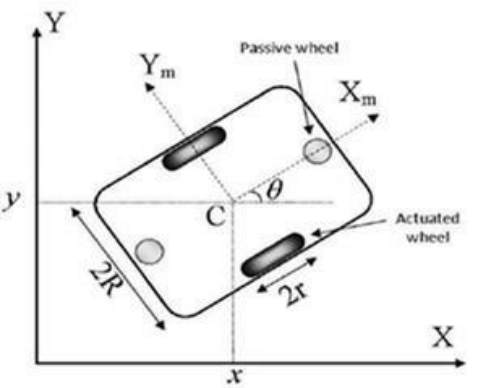
\includegraphics[width=\linewidth]{dwg/robot.png}
  \caption{Unicycle Kinematic Model}
 
\end{figure}

for each agent the states and controls can be written in vectorial form:

$$ \mathbf{s_{i}} =  \begin{bmatrix} x_{i}\\ y_{i} \\ \phi_{i}  \end{bmatrix}\in \real^{3} $$
$$ \mathbf{u_{i}} =  \begin{bmatrix} v_{i}\\ \omega{i}  \end{bmatrix} \in \real^{2}$$


So the full dynamical model can be written in matrix form as:


$$ \mathbf{s_{i}}(k+1)  = \begin{bmatrix}1 & 0 & 0 \\ 0  & 1 & 0\\ 0&0&1 \end{bmatrix}
\mathbf{s_{i}}(k)+\begin{bmatrix}cos(\phi_{i}(k)) & 0  \\ sin(\phi_{i}(k)) & 0\\ 0&1& \end{bmatrix}\mathbf{u_{i}}(k) \delta t$$


At least one of the agents is provided with a GPS system that is necessary to get an absolute measurement, else it will be not possible to univocally describe the position of the agents network in space, a camera is used to measure the absolute orientation of that agent to have an absolute measurement of the angle.
Moreover each agent is equipped with sensors able to perform a relative measurements of another agent with respect to its position. Cameras are used to get the relative orientation of the robot.
Every agent has a bounded communication range. Communications can happen either in a single broadcast to the entire team or in multi-hop fashion, i.e., every agent rebroadcasts every received message intended to reach the entire team. Each robot has
a detectable unique identifier which, as explained in the notation section in this paper is defined as the apex and is an integer number i.


\section{Extended Kalman Filter}


\begin{figure}[H]
 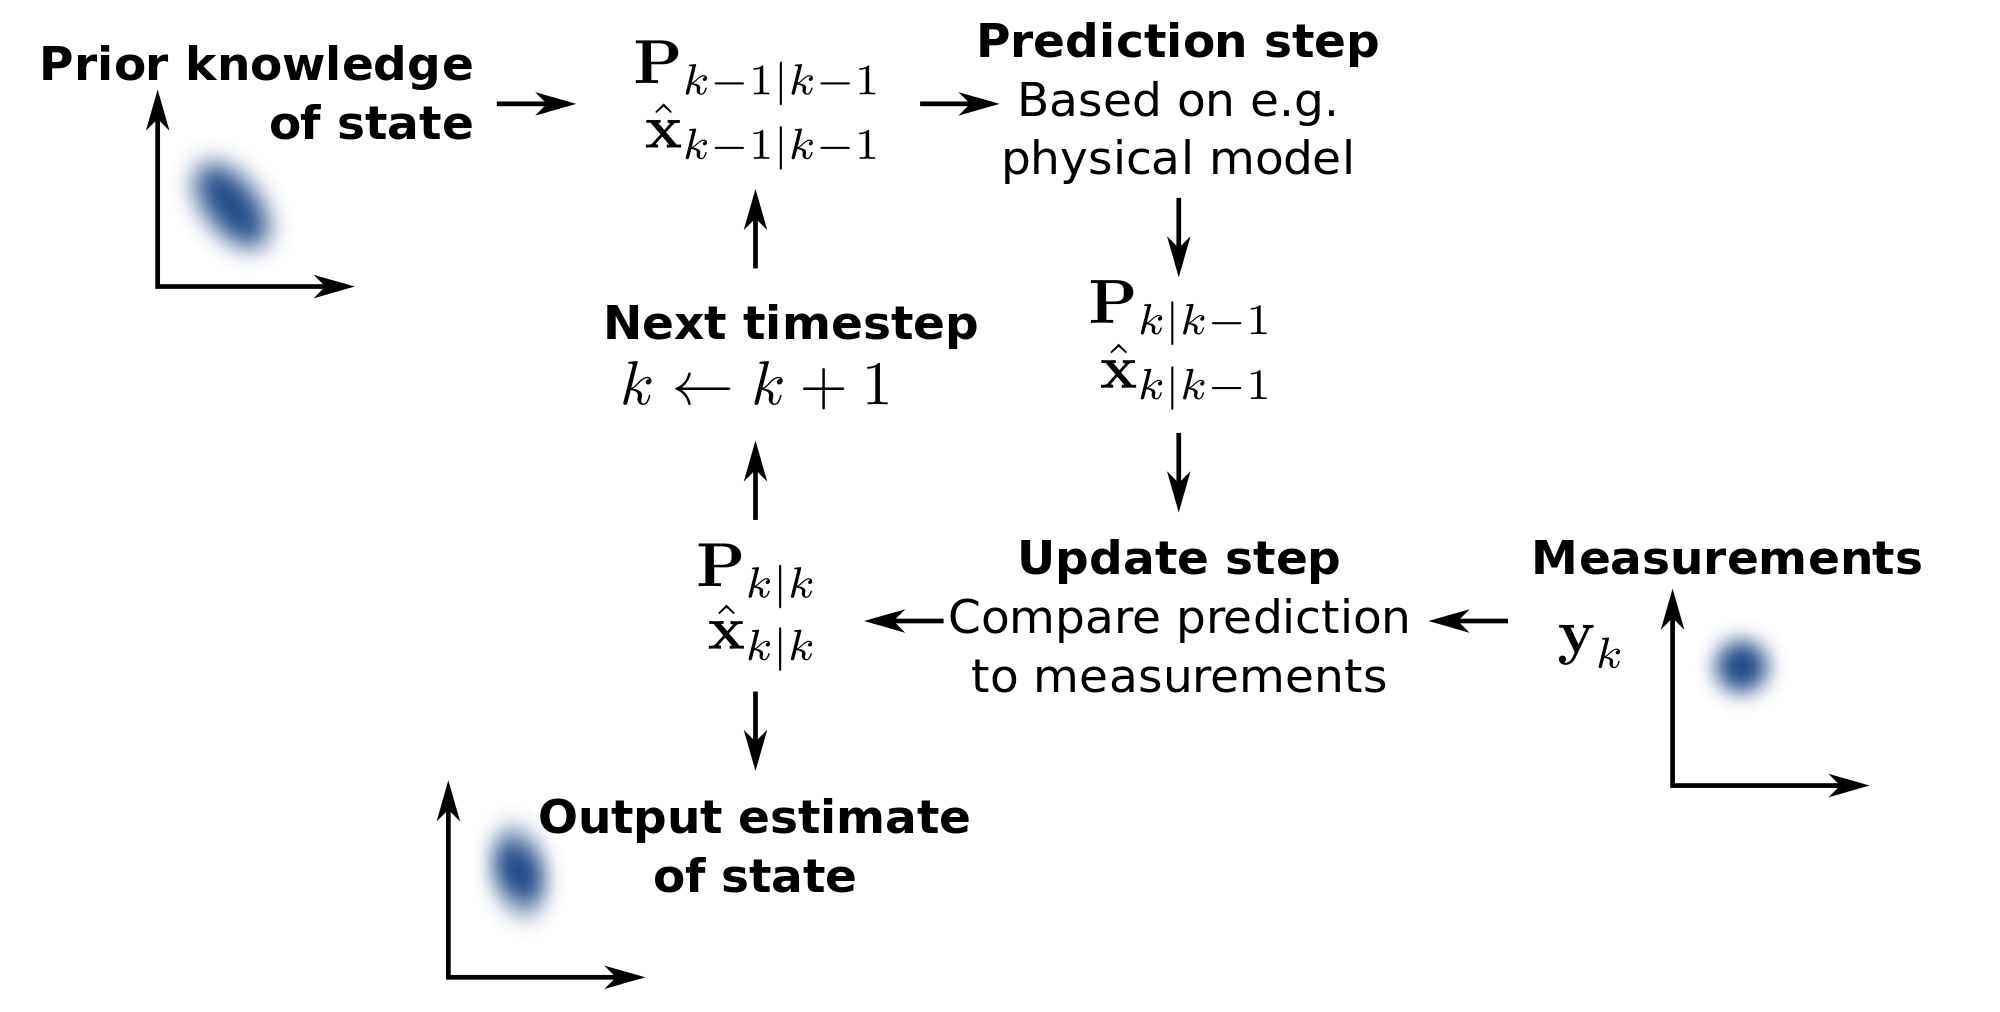
\includegraphics[width=\linewidth]{dwg/kalman.png}
  \caption{Kalman Filter structure} 
\end{figure}

Consider a team of N agents as the one modeled in the previous section. Using a set of so-called proprioceptive
sensors every agent i measures its self-motion and uses it to propagate its equations of
motion as follow:

$$  \mathbf{s_{i}}(k+1) =  \mathbf{f_{i}}(\mathbf{s_{i}}(k), \mathbf{u_{i}}(k))+\mathbf{g_{i}}(\mathbf{s_{i}}(k))\mathbf{n_{i}}(k) $$

where $ \mathbf{g_{i}}(\mathbf{x_{i}}(k))$ and $ \mathbf{n_{i}}(k)$ are respectively the process noise coefficient and process noise vector of the agent i;

The full state of the group of agents at time k can be written as:

$$  \mathbf{q}(k+1) =  \mathbf{f}(\mathbf{q}(k), \mathbf{u}(k))+\mathbf{g}(\mathbf{q}(k))\mathbf{n}(k) $$

Where:

$$ \mathbf{q}  = \begin{bmatrix}  \mathbf{\hat{s}_{1}}  \\  \vdots \\  \mathbf{\hat{s}_{N}}  \end{bmatrix} \in \real^{3N} $$

and $\mathbf{f}(\mathbf{q}(k))$ = $[\mathbf{f_{1}}(\mathbf{s_{1}}(k), \mathbf{u_{1}}(k))$ ...$ \mathbf{f_{N}}(\mathbf{s_{N}}(k), \mathbf{u_{N}}(k))]^{T}$ and $\mathbf{g}(\mathbf{q}(k))$ = Diag$[\mathbf{g_{1}}(\mathbf{s_{1}}(k))$ ...$ \mathbf{g_{N}}(\mathbf{s_{N}}(k))]$

It is clear from the equation that if each agents only relies in the proprioceptive sensors to propagate the states of all the agents the estimation of the full state will diverge cause of the noise.
A proprioceptive measurement (GPS) is modeled as:

$$  \mathbf{z_{i}}(k+1) =  \mathbf{h_{i}}(\mathbf{s_{i}}(k))+\mathbf{\nu_{g}}(k) $$

\begin{figure}[H]
 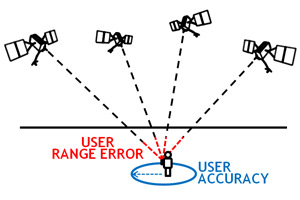
\includegraphics[width=\linewidth]{dwg/gps.jpg}
  \caption{GPS measurement model}
 
\end{figure}

Where $\nu_{g}$ is the measurement noise for the GPS in the agent and  $\mathbf{h_{i}}$ is the measurement model of the agent.
There comes into play the presence of the exeroceptive sensors of the agents which are used to take relative measurement of the pose of another agent in the network. Let us denote the relative measurement as:

$$  \mathbf{z_{ij}}(k+1) =  \mathbf{h_{ij}}(\mathbf{s_{i}}(k), \mathbf{s_{j}}(k))+\mathbf{\nu}(k) $$

\begin{figure}[H]
 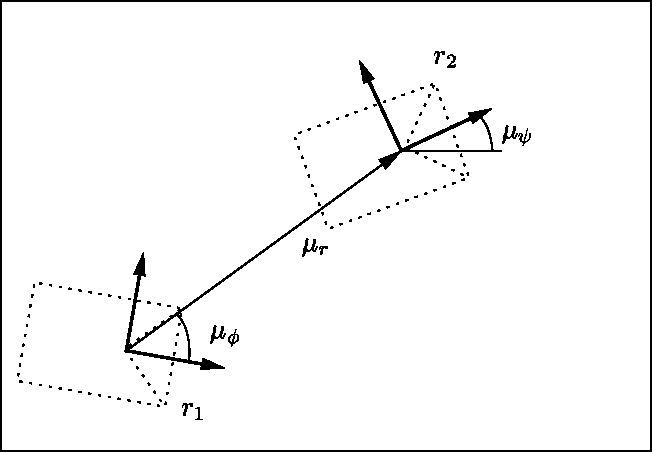
\includegraphics[width=\linewidth]{dwg/relative.png}
  \caption{Relative measurement model}
 
\end{figure}

Here $\mathbf{h_{ij}}$ is the measurement model of the agent and $\nu$ is the measurement noise of agent i, that will be assumed as a white zero-mean gaussian process since it is a necessary condition to assure convergence of the Kalman filter.
The main difference between the usage of relative measurements and absolute ones is the presence of mutual covariance matrices that can't be ignored. More in detail, An agent performs a measurement of another nearby agent in the network (or a self measurement through the GPS) and proceeds in applying the steps of the EKF as both agents are part of the same system. In this context, the prediction step is as follow:

$$  \mathbf{\hat{q}^{-}}(k+1) =  \mathbf{f}(\mathbf{\hat{q}^{+}}(k), \mathbf{u}(k)) $$

$$  \mathbf{\hat{P}^{-}}(k+1) =  \mathbf{A}(k)\mathbf{\hat{{P}}^{+}}(k)\mathbf{A}(k)^{T} + \mathbf{B}(k)\mathbf{{Q}}(k) \mathbf{B}(k)^{T} $$

Where $\mathbf{B}(k)$=$\pdv {}{\mathbf{q}}\mathbf{f}(\mathbf{\hat{q}^{+}}(k), \mathbf{u}(k))$ and $\mathbf{B}(k)$=$\pdv {}{\mathbf{u}}\mathbf{g}(\mathbf{\hat{q}^{+}}(k))$.
Of course the matrix $\mathbf{\hat{P}}$ is the predicted covariance matrix of the filter which will be in the following block form:

$$  \mathbf{\hat{P}} =  \begin{bmatrix} \mathbf{\hat{P}}_{1}  & \cdots &\mathbf{\hat{P}}_{1N}   \\ \vdots & \ddots & \vdots \\ \mathbf{\hat{P}}_{1N}^{T} & \cdots & \mathbf{\hat{P}}_{N}   \end{bmatrix} \in \real^{3N \times 3N}$$

$$ \mathbf{S}(k+1) = \mathbf{R_{i}}(k+1) + \mathbf{H}(k+1)\mathbf{\hat{P}^{-}}(k+1)\mathbf{H}(k+1)^{T} $$

Here $\mathbf{R_{i}}(k+1)$ is the covariance of the observation noise which is different for every agent and of course changes between GPS measurement and relative measurement and $\mathbf{H}(k+1)$ is the Jacobian of the measurement model with respect to the agent and is defined as follow:
when a relative measurement is taken between 2 agents i and j the Jacobian is constructed as

$$ \mathbf{H_{ij}}=  \begin{bmatrix}\mathbf{0}_{3} & \cdots & \mathbf{H_{i}}& \mathbf{0}_{3}  & \cdots & \mathbf{H_{j}}& \mathbf{0}_{3} & \cdots \mathbf{0}_{3} \end{bmatrix} \in \real^{3 \times 3N}$$

While the Jacobian for self measurement is defined as:

$$ \mathbf{H_{i}}=  \begin{bmatrix}\mathbf{0}_{3} & \cdots & \mathbf{H_{i}}& \mathbf{0}_{3}  & \cdots \mathbf{0}_{3} \end{bmatrix}  \in \real^{3 \times 3N}$$

In this context we assume to take 3 measurements in both cases: the GPS measured position and the orientation measured by on board sensors for the self measurement, while the distance and for all the coordinates of 2 agents is used for the relative measurement.
then the filter proceeds to calculates the Kalman Gain:

$$\mathbf{K}(k+1) = \mathbf{\hat{P}^{-}}(k+1)\mathbf{H}(k+1)^{T}\mathbf{S}(k+1)^{-1}$$

At last, the filter will perform the update step before going back to the start of the algorithm

$$ \mathbf{\hat{q}^{+}}(k+1) = \mathbf{\hat{q}^{-}}(k+1) + \mathbf{K}(k+1)\mathbf{r}(k+1) $$
$$\mathbf{ \hat{P}^{+}}(k+1) = \mathbf{\hat{P}^{-}}(k+1) -  \mathbf{K}(k+1)\mathbf{H}(k+1) \mathbf{\hat{P}^{-}}(k+1) $$

Where $ \mathbf{r}(k+1) $ is defined for both measurements cases as:

$$\mathbf{r}(k+1)  = \mathbf{z}_{i}(k+1) -  \mathbf{h}_{i}(\mathbf{\hat{q}}_{i}^{-}(k+1))$$

$$\mathbf{r}(k+1)  =   \mathbf{z}_{ij}(k+1) -   \mathbf{h}_{ij}(\mathbf{\hat{q}}_{i}^{-}(k+1), \mathbf{\hat{q}}_{j}^{-}(k+1))$$




\section{Interacting Multiple Model Estimator}

\begin{figure}[H]
 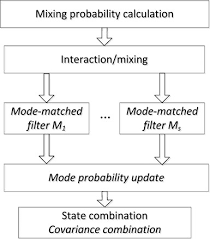
\includegraphics[width=\linewidth]{dwg/imm.png}
  \caption{Interacting Multiple Models structure} 
\end{figure}

As discussed in previous sections the Kalman filter operates on a single model for each agent. If a situation where the model of the agent can't be decided a priori, another strategy is necessary to get a better estimation of the network position. The same Kalman filter with different models can be implemented for each agent in the network and the IMM estimator will take charge of deciding which one is closer to the reality given by the measurement taken at each step. Assuming there are M models considered for the IMM estimator the following steps are taken to estimate the best model. We will utilize the IMM definition given by Bar-Shalom in \cite{Bar-Shalom}
The first step in each iteration for the multiple model estimator is to update the conditional model probabilities which are the "weigths" of each model considered in the estimation. In this paper we will assume that the IMM estimator has to choose between a set of models that is defined as $\{1..M\}$.
To update each model some definitions are required:

$$ \mathbf{\Pi} = \begin{bmatrix} p_{11} & \cdots & p_{1M} \\ \vdots & \ddots & \vdots \\ p_{M1} & \cdots & p_{MM} \end{bmatrix} \in \real^{M \times M} $$
$$ \mathbf{\hat{\mu}}^{+}(k) = \begin{bmatrix} \hat{\mu}_{1}^{+}(k) \\ \vdots \\ \hat{\mu}_{M}^{+}(k)  \end{bmatrix} \in \real^{M}$$

The matrix $ \mathbf{\Pi} $ represents the a priori probability of switching model or staying in the current model for each agent and it is usually fixed over time. While the vector $ \hat{\mathbf{\mu}}(k)$ represents the model probabilities which are the probabilities of being in the state i at time k.
Knowing $ \mathbf{\Pi} $ and  $ \hat{\mathbf{\mu}}^{+}(k)$ is necessary to build the conditional model probabilities, which are defined as $\mathbf{\hat{M}}^{-}(k+1)$:

$$ \hat{ \mathbf{M}}^{-}(k+1) = \begin{bmatrix}  \hat{\mu}_{1|1}^{-} & \cdots &  \hat{\mu}_{1|M}^{-}\\ \vdots & \ddots & \vdots \\  \hat{\mu}_{M|1}^{-} & \cdots &  \hat{\mu}_{M|M}^{-} \end{bmatrix} \in \real^{M\times M} $$

The entries of the matrix are defined as: 

$$   \hat{\mu}_{i|j}^{-}(k+1) = \frac{1}{\bar{c}_{j}(k+1)}p_{ij}\hat{\mu}_ {i}^{+}(k) $$

where: 


$$ \mathbf{\bar{c}(k+1)} =  \begin{bmatrix} \bar{c}_{1}(k+1) \\ \vdots \\  \bar{c}_{M}(k+1) \end{bmatrix}= \mathbf{\Pi}^{T}\hat{\mathbf{\mu}}^{+}(k)  \in \real^{M} $$
%$$ \bar{c}_{j}(k+1) = \sum_{i = 1}^{M} p_{ij}\hat{\mu}_ {i}^{+}(k) $$


Each iteration for the distributed Kalman filter is preceded by the State Interaction necessary for the IMM estimator, which get as input the previous step state estimated by all the filter models $\mathbf{\hat{q}^{+}}$(k) and the covariance matrix $\mathbf{ \hat{P}^{+}}$(k) for each model considered possible for the agents. 


$$ \mathbf{\hat{q}_{j}^{0}}(k+1) = \sum_{n = 1}^{M} \mathbf{\hat{q}_{n}^{+}}(k)\hat{\mu}_{n|j}^{-}(k+1) $$
$$ \mathbf{\hat{P}_{j}^{0}}(k+1) = \sum_{n = 1}^{M} \hat{\mu}_{n|j}^{-}(k+1)[\mathbf{\hat{ P}_{j}^{+}}(k)$$
$$+( \mathbf{\hat{q}_{n}^{+}}(k) -  \mathbf{\hat{q}_{j}^{0}}(k+1))( \mathbf{\hat{q}_{n}^{+}}(k) -  \mathbf{\hat{q}_{j}^{0}}(k+1))^{T} ] $$

The results for the State interaction step will feed the corresponding filter model, each filter then will be updated using relative or absolute measurements. Then the model probabilities are updated using the residual covariance and the relative measurements.

$$ \Lambda_{j}(k+1) = \frac{1}{\sqrt{2\pi\abs{ S_{j}}}} e^{-\frac{1}{2}s_{j}(k+1)} $$ 

Where:

$$ s_{j}(k+1) = \mathbf{r}_{j}^{T}(k+1)\mathbf{S}_{j}^{-1}(k+1)\mathbf{r}_{j}(k+1) \in \real $$ 

The so called Likelihood function $ \Lambda$ gives a normal distribution that tends to represent the value of inputs given the output values of the system and it can be used to update the model probabilities of the IMM estimator.

$$ \hat{\mu_{j}}^{+}(k+1) = \frac{1}{\sum_{n=1}^{M}\Lambda_{n} \bar{c}_{n}}  \Lambda_{j} \bar{c}_{j}$$

In the end the result of each single Kalman filter will be used to restart the iteration with the next update on the conditional model probabilities and the State interaction. There will also be a parallel step called State Combination where the output of each Kalman filter will be combined to get the best estimation of the agent position. It can be proved that this result will be better than the results of the single Kalman filter if one the model used in the IMM estimator matches the real behaviour of the agents.

 
$$ \mathbf{\hat{Q}}(k+1) = \sum_{n = 1}^{M} \mathbf{\hat{q}_{n}^{+}}(k+1)\mathbf{\hat{\mu}}_{n}^{+}(k+1) $$
$$ \mathbf{P}(k+1) = \sum_{n = 1}^{M} \mathbf{\hat{\mu}}_{n}^{+}(k+1)[\mathbf{\hat{ P}_{n}^{+}}(k+1)$$
$$+( \mathbf{\hat{q}_{n}^{+}}(k+1) -  \mathbf{\hat{Q}}(k+1))( \mathbf{\hat{q}_{n}^{+}}(k+1) -  \mathbf{\hat{Q}}(k+1))^{T} ] $$


\section{Centralized EKF Extension}

Exploring the previosly explained Kalman Filter matrices, it is possible to find some patterns, which can be exploited to put the model in the so called centralized form. The difference between the two is basically the possibility of not considering the whole set of agents as one unique system but to decouple them. In this model, one of the agents is declared as the one in charge to take all the relative measurements and it is the only one that needs to have an absolute reference (GPS measurements) to have an observable system that present no ambiguity. That same agent is in charge of developing all the filter steps, while possibly communicating to the others the result of each step.
Starting from the first step of the Kalman filter, we will try to decouple the matrices where it is possible. This process will conclude with a formulation which is equivalent to the one shown by Kia et al. in \cite{Kia-Martinez}

$$  \mathbf{\hat{q}^{-}}(k+1) =  \mathbf{f}(\mathbf{\hat{q}^{+}}(k), \mathbf{u}(k)) $$

$$  \mathbf{\hat{P}^{-}}(k+1) =  \mathbf{A}(k)\mathbf{\hat{P}^{+}}(k)\mathbf{A}(k)^{T} + \mathbf{B}(k)\mathbf{{Q}}(k) \mathbf{B}(k)^{T} $$

The first equation can be easily separated by splitting the vectors in each agents own states vector:

$$  \mathbf{\hat{q}_{i}^{-}}(k+1) =  \mathbf{f}(\mathbf{\hat{q}_{i}^{+}}(k), \mathbf{u}_{i}(k)) $$

The first pattern in the block matrices we can find is present in the prediction for the covariance matrix $\mathbf{\hat{P}}^{-}(k+1)$:

 $$ \mathbf{A}(k) =  \begin{bmatrix} \mathbf{A}_{1} &  \mathbf{0}_{3} &\cdots & \mathbf{0}_{3} \\  \mathbf{0}_{3} & \mathbf{A}_{2} &  \mathbf{0}_{3} & \vdots \\ \vdots & \vdots & \ddots & \vdots \\ \mathbf{0}_{3} &  \mathbf{0}_{3} &\cdots& \mathbf{A}_{N} \end{bmatrix}$$

 $$ \mathbf{B}(k) =  \begin{bmatrix} \mathbf{B}_{1} &  \mathbf{0}_{32} &\cdots & \mathbf{0}_{32} \\  \mathbf{0}_{32} & \mathbf{B}_{2} &  \mathbf{0}_{32} & \vdots \\ \vdots & \vdots & \ddots & \vdots \\ \mathbf{0}_{32} &  \mathbf{0}_{32} &\cdots& \mathbf{B}_{N} \end{bmatrix}$$

 $$ \mathbf{\hat{P}}^{+}(k) =  \begin{bmatrix} \mathbf{\hat{P}}_{1} &  \mathbf{\hat{P}}_{12} &\cdots & \mathbf{\hat{P}}_{1N} \\  \mathbf{\hat{P}}_{12}^{T} & \mathbf{\hat{P}}_{2} &  \cdots & \mathbf{\hat{P}}_{2N} \\ \vdots & \vdots & \ddots & \vdots \\ \mathbf{\hat{P}}_{1N}^{T} &  \cdots &\cdots& \mathbf{\hat{P}}_{N} \end{bmatrix}$$

Developing the dot product between matrices it is possible to have smaller covariance matrices for single agents and the reciprocal covariance matrices between 2 agents. Then for each agent i we have:

$$  \mathbf{\hat{P}}_{i}^{-}(k+1) =  \mathbf{A}_{i}(k)\mathbf{{\hat{P}}_{i}^{+}}(k)\mathbf{A}_{i}(k)^{T} + \mathbf{B}_{i}(k)\mathbf{Q}_{i}(k) \mathbf{B}_{i}(k)^{T} $$

While for the reciprocal covariance between two robots i and j we have:

$$  \mathbf{\hat{P}}_{ij}^{-}(k+1) =  \mathbf{A}_{i}(k)\mathbf{{\hat{P}}_{ij}^{+}}(k)\mathbf{A}_{j}(k)^{T} $$

Now we can exploit the same block matrix structure to separate the Gains of the Kalman Filter for each agent and to simplify the residual covariance matrix calculation. We have explored the block structure of the $\mathbf{H}(k+1)$ in section 4 let's apply the dot product between matrices to the equation for the residual covariance matrix $\mathbf{S}(k+1)$:

$$ \mathbf{S}(k+1) = \mathbf{R_{i}}(k+1) + \mathbf{H}(k+1)\mathbf{\hat{P}}^{-}(k+1)\mathbf{H}(k+1)^{T} $$

This can be written as:

$$ \mathbf{S}(k+1) = \mathbf{R_{ij}}(k+1) + \mathbf{H}_{i}(k+1)\mathbf{\hat{P}}_{i}^{-}(k+1)\mathbf{H}_{i}^{T}(k+1)$$
$$ +\mathbf{H}_{j}(k+1)\mathbf{\hat{P}}_{j}^{-}(k+1)\mathbf{H}_{j}^{T}(k+1)$$
$$ - \mathbf{H}_{i}(k+1)\mathbf{\hat{P}}_{ij}^{-}(k+1)\mathbf{H}_{j}^{T}(k+1)$$
$$ - \mathbf{H}_{j}(k+1)\mathbf{\hat{P}}_{ij}^{-T}(k+1)\mathbf{H}_{i}^{T} (k+1)$$

The minus sign comes from the definition of the $\mathbf{H}_{i}(k+1)$ since usually the cartesian distance of the 2 robots is used for a relative measurements the one who takes the measurements is negative. To define a positive matrix in this dissertation the sign is considered outside of the Matrix.
The self measurement case is trivial as it becomes:

$$ \mathbf{S}(k+1) = \mathbf{R_{i}}(k+1) + \mathbf{H}_{i}(k+1)\mathbf{\hat{P}}_{i}^{-}(k+1)\mathbf{H}_{i}^{T}(k+1)$$

Next step is to separate the Kalman gain of the agents from each other. This will require the same approach as seen up to now and yield the following results:

$$\mathbf{K}_{i}(k+1) = [\mathbf{\hat{P}}_{ij}^{-}(k+1)\mathbf{H}_{j}^{T}(k+1)$$
$$-\mathbf{\hat{P}}_{i}^{-}(k+1)\mathbf{H}_{i}^{T}(k+1)]\mathbf{S}(k+1)^{-1}$$

$$\mathbf{K}_{j}(k+1) = [\mathbf{\hat{P}}_{j}^{-}(k+1)\mathbf{H}_{j}^{T}(k+1)$$
$$-\mathbf{\hat{P}}_{ij}^{-}(k+1)^{T}\mathbf{H}_{i}^{T}(k+1)]\mathbf{S}(k+1)^{-1}$$

For the agents that don't take part in the measurement we have:

$$\mathbf{K}_{k}(k+1) = [\mathbf{\hat{P}}_{kj}^{-}(k+1)\mathbf{H}_{j}^{T}(k+1)-$$
$$\mathbf{\hat{P}}_{ki}^{-}(k+1)\mathbf{H}_{i}^{T}(k+1)]\mathbf{S}(k+1)^{-1}$$

It is easy to find the equation for the updated state of each agent that come simply from the old equation:

$$ \mathbf{\hat{q}}_{i}^{+}(k+1) = \mathbf{\hat{q}}_{i}^{-}(k+1) + \mathbf{K}_{i}(k+1)\mathbf{r}(k+1) $$

Last step requires to separate the Gain matrices that will be added to the predicted covariance matrices to find the updated ones.

$$\mathbf{\hat{ P}}^{+}(k+1) = \mathbf{\hat{P}}^{-}(k+1) -  \mathbf{K}(k+1)\mathbf{H}(k+1) \mathbf{\hat{P}}^{-}(k+1) $$

Notice that since the matrix of the Kalman Gain is written as:

$$\mathbf{K}(k+1) = \mathbf{\hat{P}^{-}}(k+1)\mathbf{H}(k+1)^{T}\mathbf{S}(k+1)^{-1}$$ 

if we perform the product:

$$\mathbf{K}(k+1)\mathbf{S}(k+1)\mathbf{K}(k+1)^{T}$$ 

We get:

$$\mathbf{\hat{P}^{-}}(k+1)\mathbf{H}(k+1)^{T}\mathbf{S}(k+1)^{-1}\mathbf{S}(k+1)\mathbf{S}(k+1)^{-T}\mathbf{H}(k+1)\mathbf{\hat{P}}^{-}(k+1)^{T}$$

Since $\mathbf{\hat{P}^{-}}(k+1)= \mathbf{\hat{P}^{-}}(k+1)^{T}$, $\mathbf{S}(k+1)^{-T} = \mathbf{S}(k+1)^{-1}$ we can simplify and get:

$$  \mathbf{K}(k+1)\mathbf{H}(k+1) \mathbf{\hat{P}}^{-}(k+1) $$

Which is exactly the term we needed to update the covariance matrix in the Kalman Filter. Then let's write the Update step in this new form:

$$ \mathbf{\hat{q}}^{+}(k+1) = \mathbf{\hat{q}}^{-}(k+1) + \mathbf{K}(k+1)\mathbf{r}(k+1) $$
$$\mathbf{ \hat{P}}^{+}(k+1) = \mathbf{\hat{P}}^{-}(k+1) -  \mathbf{K}(k+1)\mathbf{S}(k+1) \mathbf{K}(k+1)^{T} $$

And then split both above relations for each agent in the network as:


$$ \mathbf{\hat{q}}_{i}^{+}(k+1) = \mathbf{\hat{q}}_{i}^{-}(k+1) + \mathbf{K}_{i}(k+1)\mathbf{r}(k+1) $$
$$\mathbf{ \hat{P}}_{i}^{+}(k+1) = \mathbf{\hat{P}}_{i}^{-}(k+1) -  \mathbf{K}_{i}(k+1)\mathbf{S}(k+1) \mathbf{K}_{i}^{T}(k+1) $$

While for the cross covariance matrices we get:

$$\mathbf{\hat{ P}}_{ij}^{+}(k+1) = \mathbf{\hat{P}}_{ij}^{-}(k+1) -  \mathbf{K}_{i}(k+1)\mathbf{S}(k+1) \mathbf{K}_{j}^{T}(k+1)$$

It is necessary to remind that in the case of GPS measurements, there is no need to change the sign of the $ \mathbf{H}_{i} $ since the measurement function is no longer defined as a distance but as a direct measurement. Moreover the Jacobian Matrix of the second agent will be defined as $ \mathbf{H}_{j}= \mathbf{0}_{3} $.

\section{Centralized IMM Esitmator}

Next step will be finding a centralized version of the IMM estimator, starting from the State Interaction, let's expand the equation to have a better idea on the necessary steps, in this section, the first index will represent the model of the IMM while the second index will reprensent the agent. So for each model we have:

$$  \mathbf{\hat{q}_{j}}(k+1) = \begin{bmatrix} \mathbf{\hat{q}_{j,1}}(k+1) \\ \vdots \\ \mathbf{\hat{q}_{j,N}}(k+1) \end{bmatrix} \in \real^{M}$$

Then we can write the relation for each agent in each model

$$ \mathbf{\hat{q}_{j,i}^{0}}(k+1) = \sum_{n = 1}^{M} \mathbf{\hat{q}_{n,i}^{+}}(k)\hat{\mu}_{n|j}^{-}(k+1) $$

From the previous section we can write:

$$\mathbf{\hat{P}_{n|j}}(k+1) = ( \mathbf{\hat{q}_{n}^{+}}(k) -  \mathbf{\hat{q}_{j}^{0}}(k+1))( \mathbf{\hat{q}_{n}^{+}}(k) -  \mathbf{\hat{q}_{j}^{0}}(k+1))^{T}  $$

and then,

$$ \mathbf{\hat{P}_{j}^{0}}(k+1) = \sum_{n = 1}^{M} \hat{\mu}_{n|j}^{-}(k+1)[\mathbf{\hat{ P}_{j}^{+}}(k)+\mathbf{\hat{P}_{n|j}}(k+1)  ] $$

For the sake of semplicity let's drop the j index and work on a single model, since the equation will be the same for each of them and sum up the 2 covariance matrix:

$$ \mathbf{\hat{P}^{0}}(k+1) = \sum_{n = 1}^{M} \hat{\mu}_{n}^{-}(k+1)\mathbf{\hat{P}_{n}}(k+1)  $$

Expanding the Full matrix of covariances for each agent we get:

$$ \mathbf{\hat{P}}_{n} =  \begin{bmatrix}  \hat{\mu}_{n}^{-}\mathbf{\hat{P}}_{n,1}  & \cdots & \hat{\mu}_{n}^{-}\mathbf{\hat{P}}_{n,1N}   \\ \vdots & \ddots & \vdots \\  \hat{\mu}_{n}^{-}\mathbf{\hat{P}}_{n,1N}^{T} & \cdots &  \hat{\mu}_{n}^{-}\mathbf{\hat{P}}_{n,N}   \end{bmatrix} $$

Picking the single covariance matrix and cross covariance and summing over n we get:

$$ \mathbf{\hat{P}_{ij}^{0}}(k+1) = \sum_{n = 1}^{M} \hat{\mu}_{n}^{-}(k+1)\mathbf{\hat{P}_{n,ij}^{+}}(k)  $$

With the previous equation each agent can update its covariance and cross covariance matrix for each model of the IMM, but it is necessary to highlight that the agent needs to know full state vector of all the agents to compute $ \mathbf{\hat{P}_{n|j}}(k+1)$ which in the Centralized version of the Kalman Filter is not necessary to proceeds in the steps for the single agent.
The above steps can be replicated for the State combination that provides the Output of the IMM estimator at each step.

$$ \mathbf{\hat{Q}_{j,i}}(k+1) = \sum_{n = 1}^{M} \mathbf{\hat{q}_{n,i}^{-}}(k+1)\hat{\mu}_{n|j}^{+}(k+1) $$
$$ \mathbf{P_{ij}}(k+1) = \sum_{n = 1}^{M} \hat{\mu}_{n}^{+}(k+1)\mathbf{\hat{P}_{n,ij}^{-}}(k+1)  $$


\section{Simulation}

First of all let's show the simulation result for the predicted trajectories of the agents: in the dwg below we can see the predicted states with respect to the real state of the system in the case of the Centralized EKF and the Output for the IMM estimator combination. Since both agent follow the same trajectories in the figures, we can see the results for the agent 1 which are qualitatively the same as the ones for agent 2.


\begin{figure}[H]
 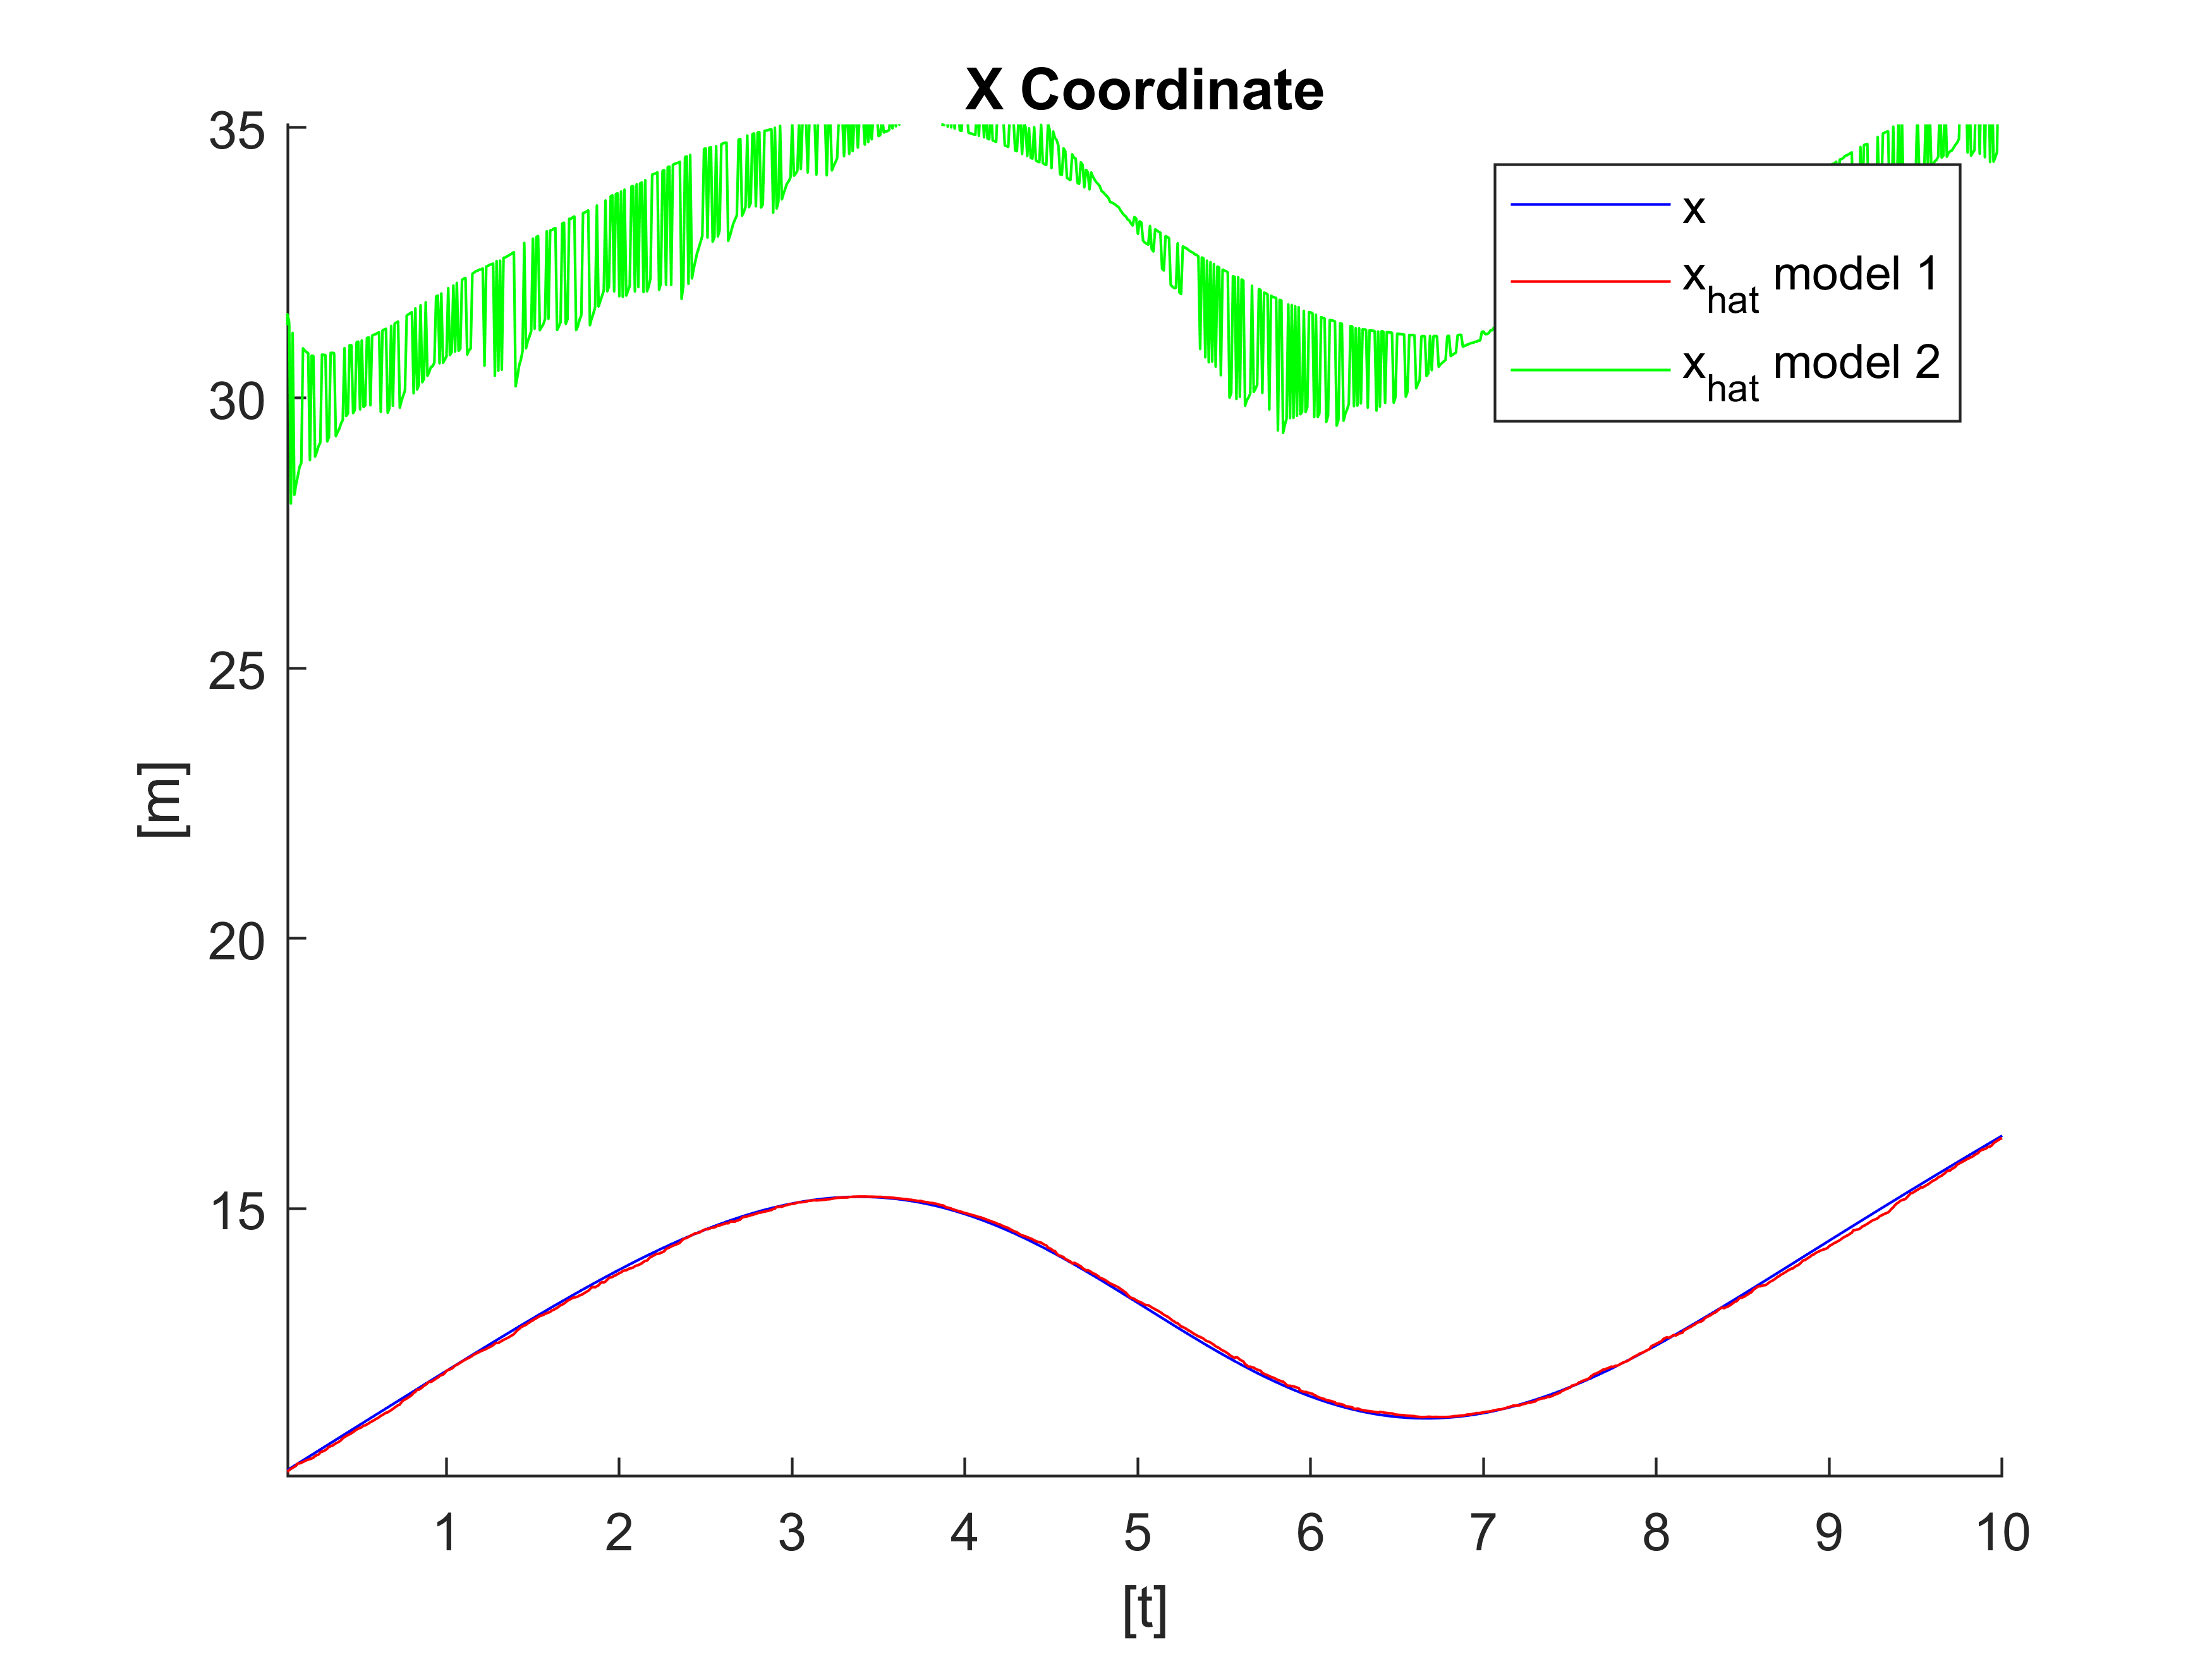
\includegraphics[width=\linewidth]{dwg/x-coord.png}
  \caption{EKF - X coordinates}
 \label{fig:first}
\end{figure}
\bigskip \bigskip \bigskip \bigskip \bigskip \bigskip \bigskip \bigskip \bigskip \bigskip 
\begin{figure}[H]
 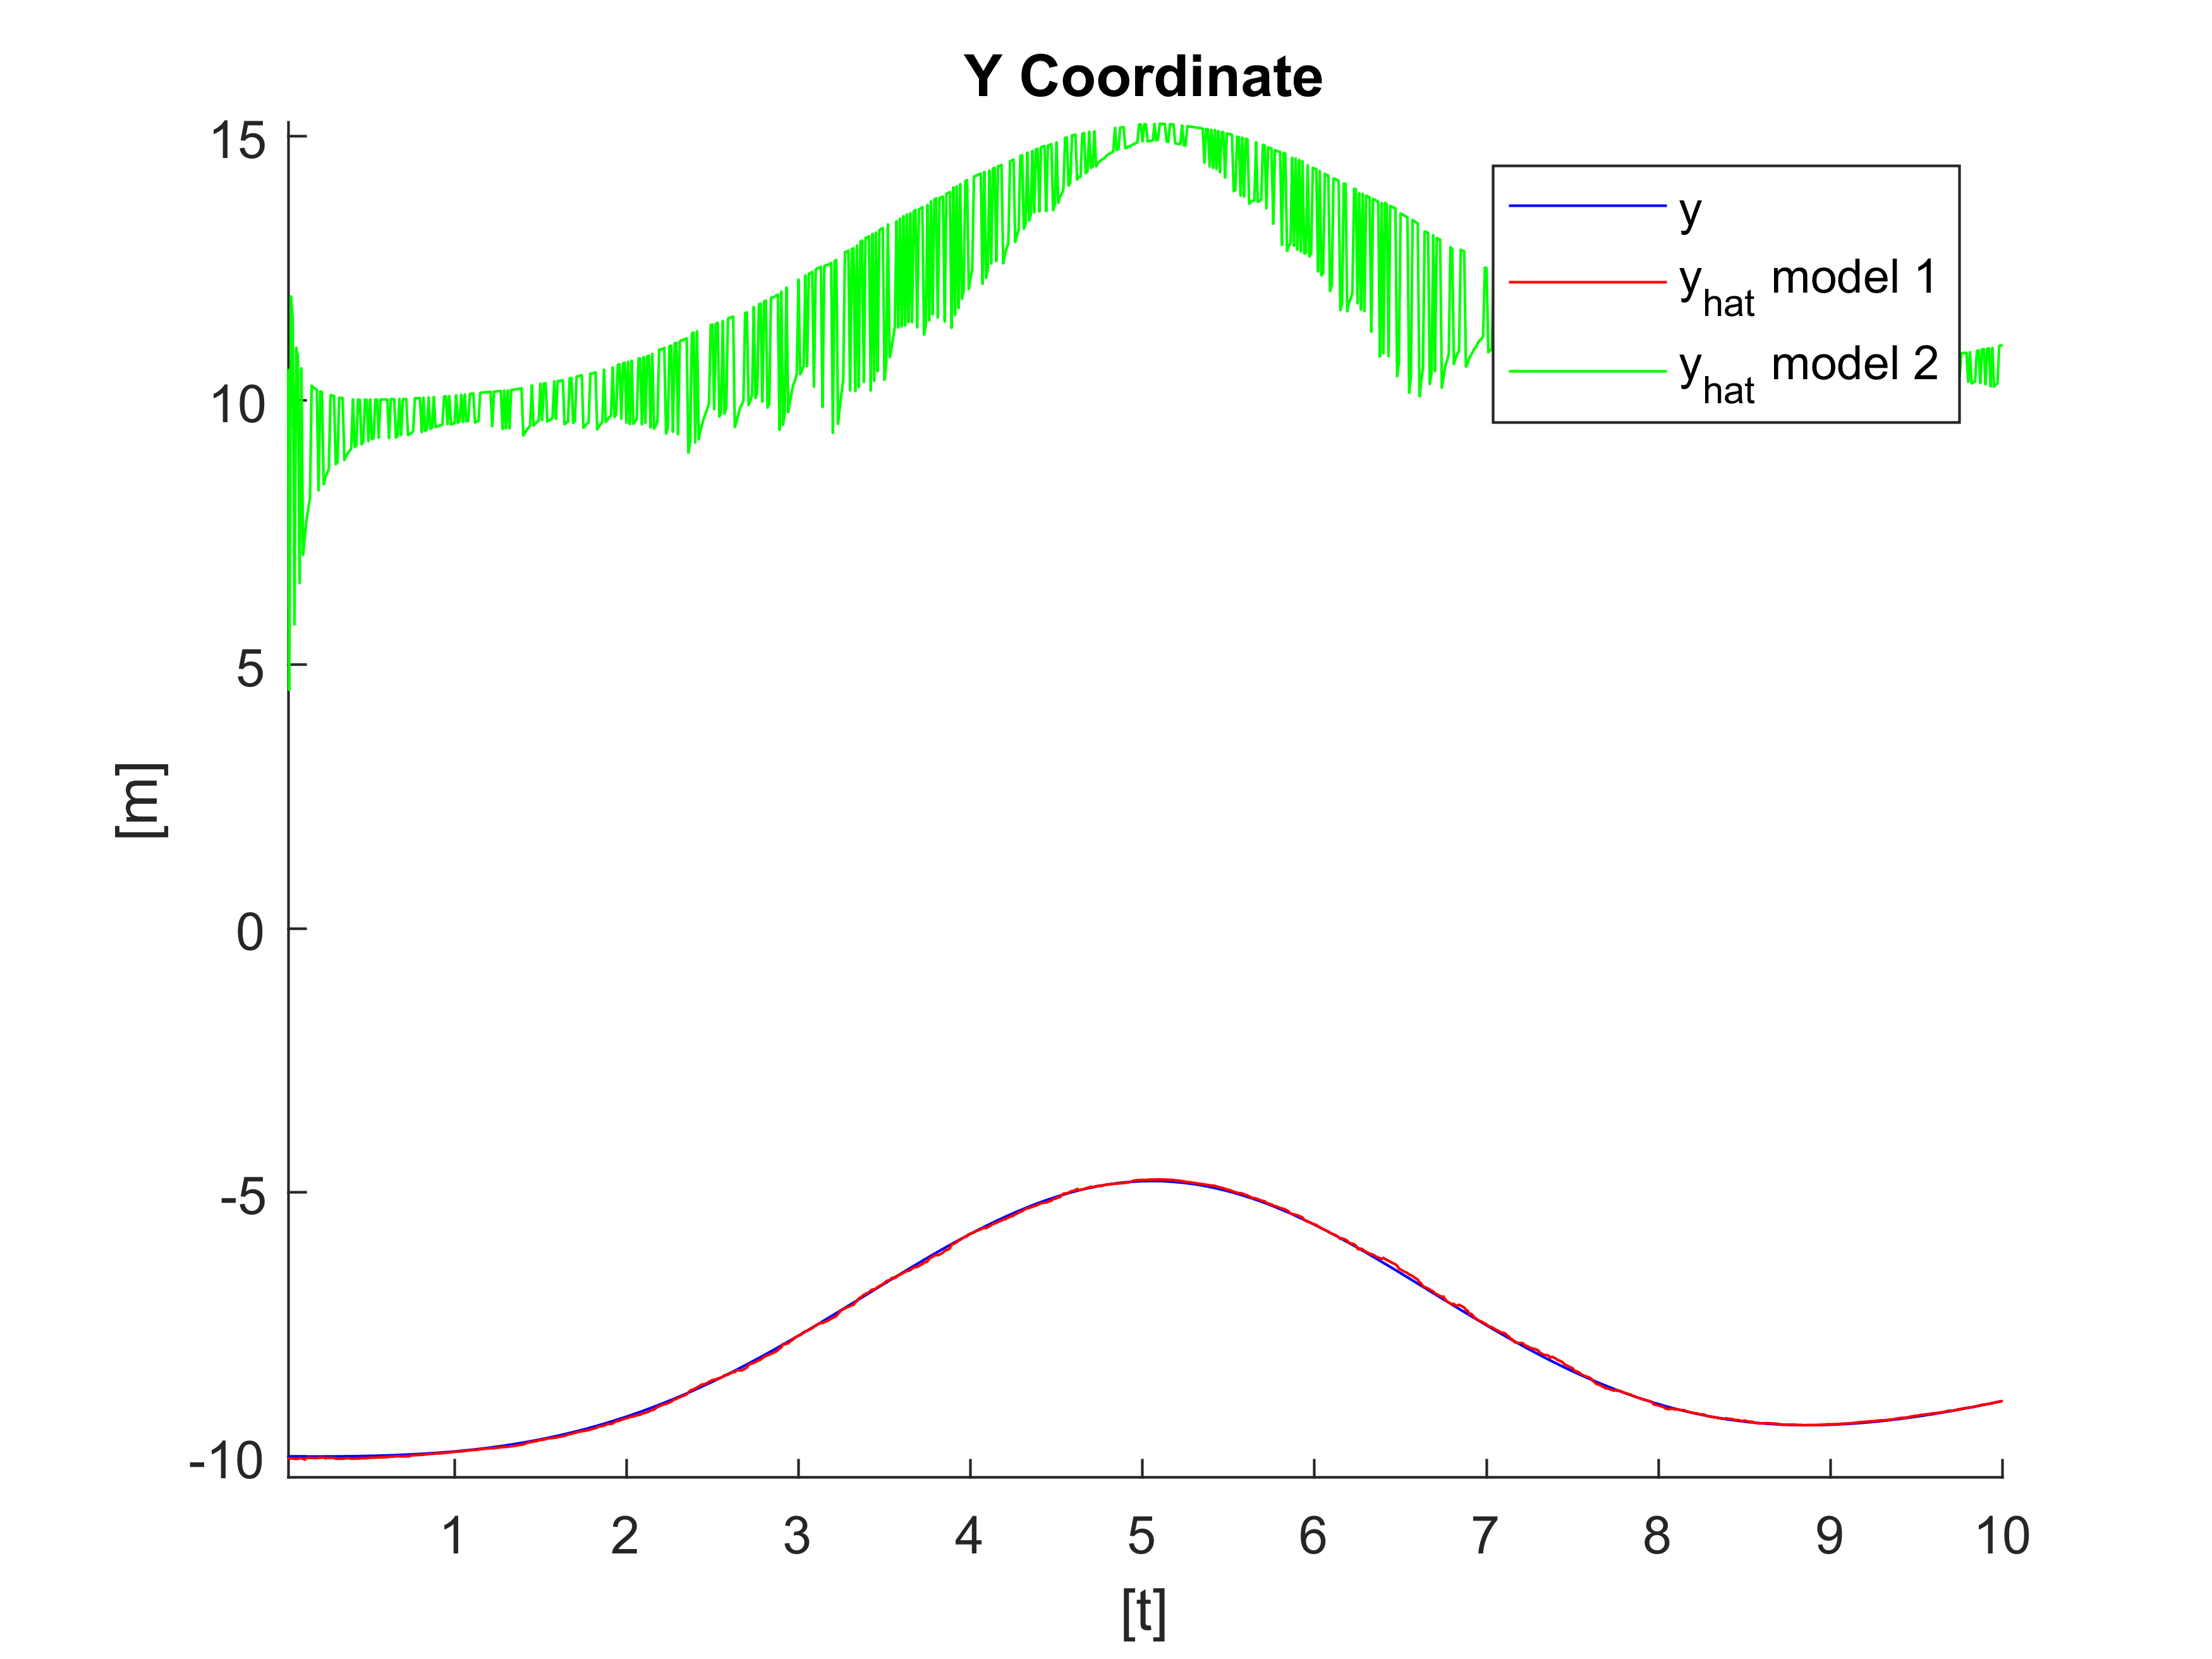
\includegraphics[width=\linewidth]{dwg/y-coord.png}
  \caption{EKF - Y coordinates}
 
\end{figure}
\bigskip \bigskip \bigskip \bigskip \bigskip \bigskip \bigskip \bigskip \bigskip \bigskip \bigskip \bigskip \bigskip \bigskip \bigskip \bigskip 
\begin{figure}[H]
 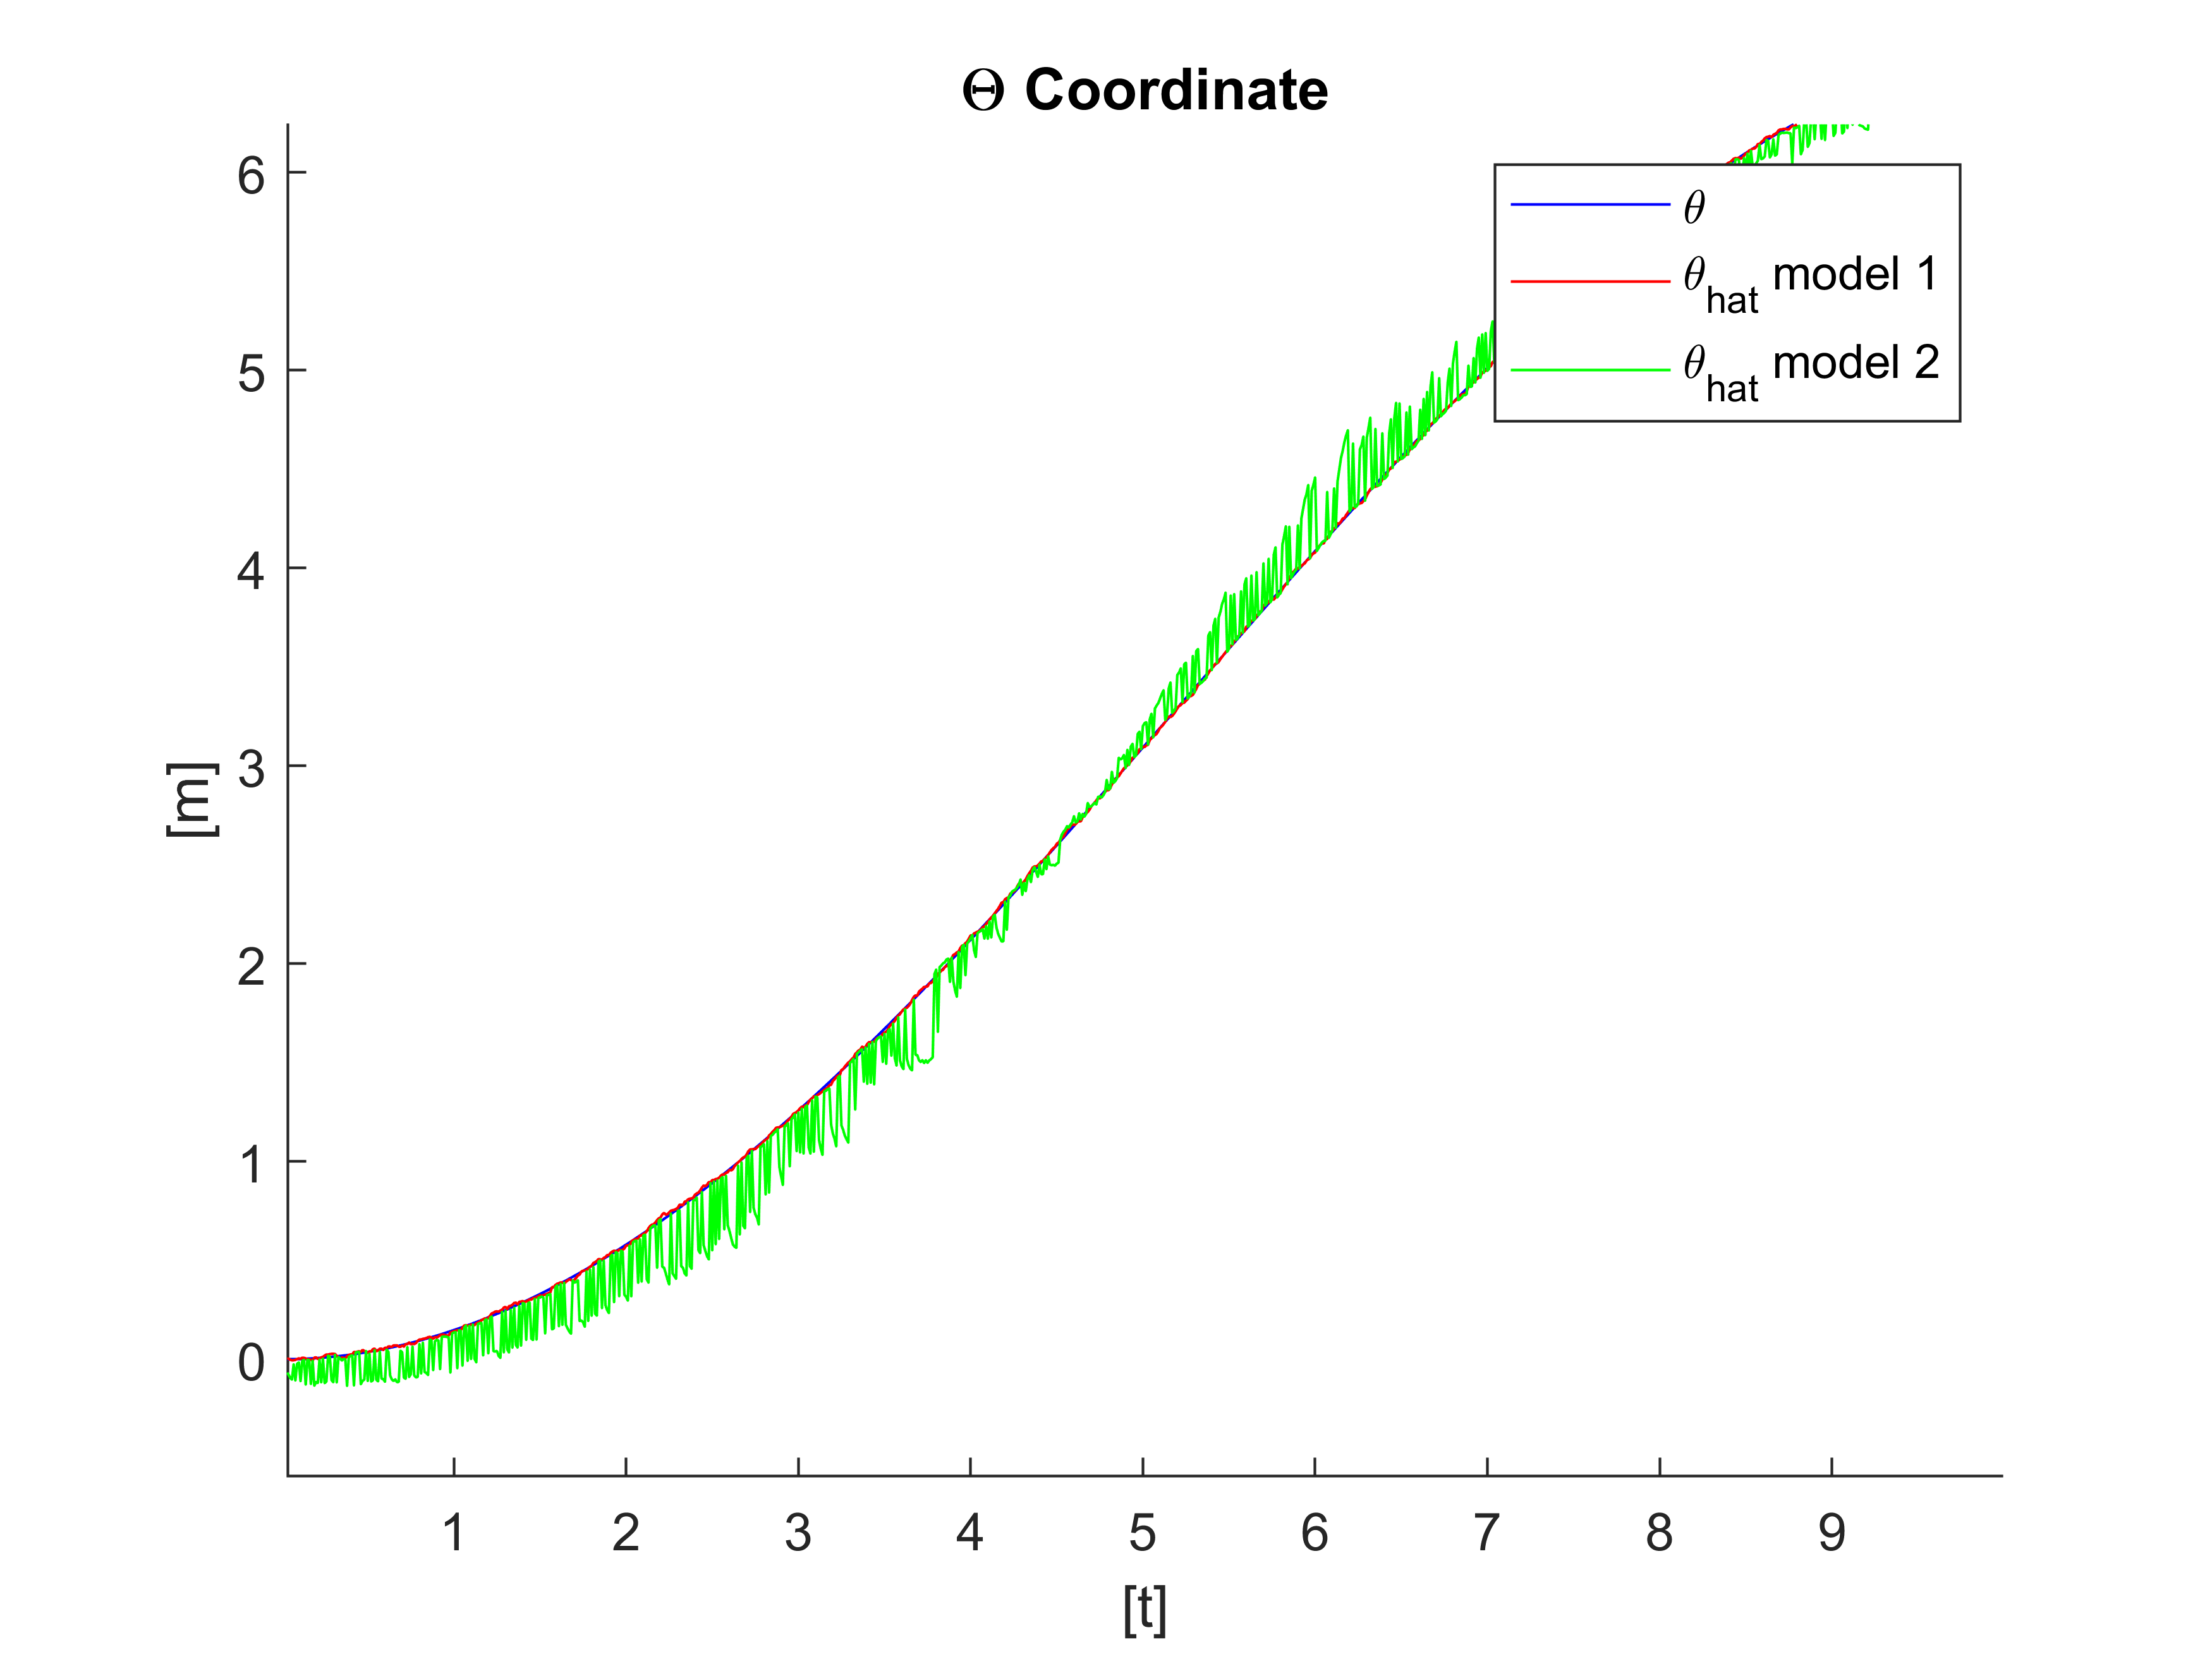
\includegraphics[width=\linewidth]{dwg/t-coord.png}
  \caption{EKF - $\Theta$ coordinates}
 
\end{figure}

\begin{figure}[H]
 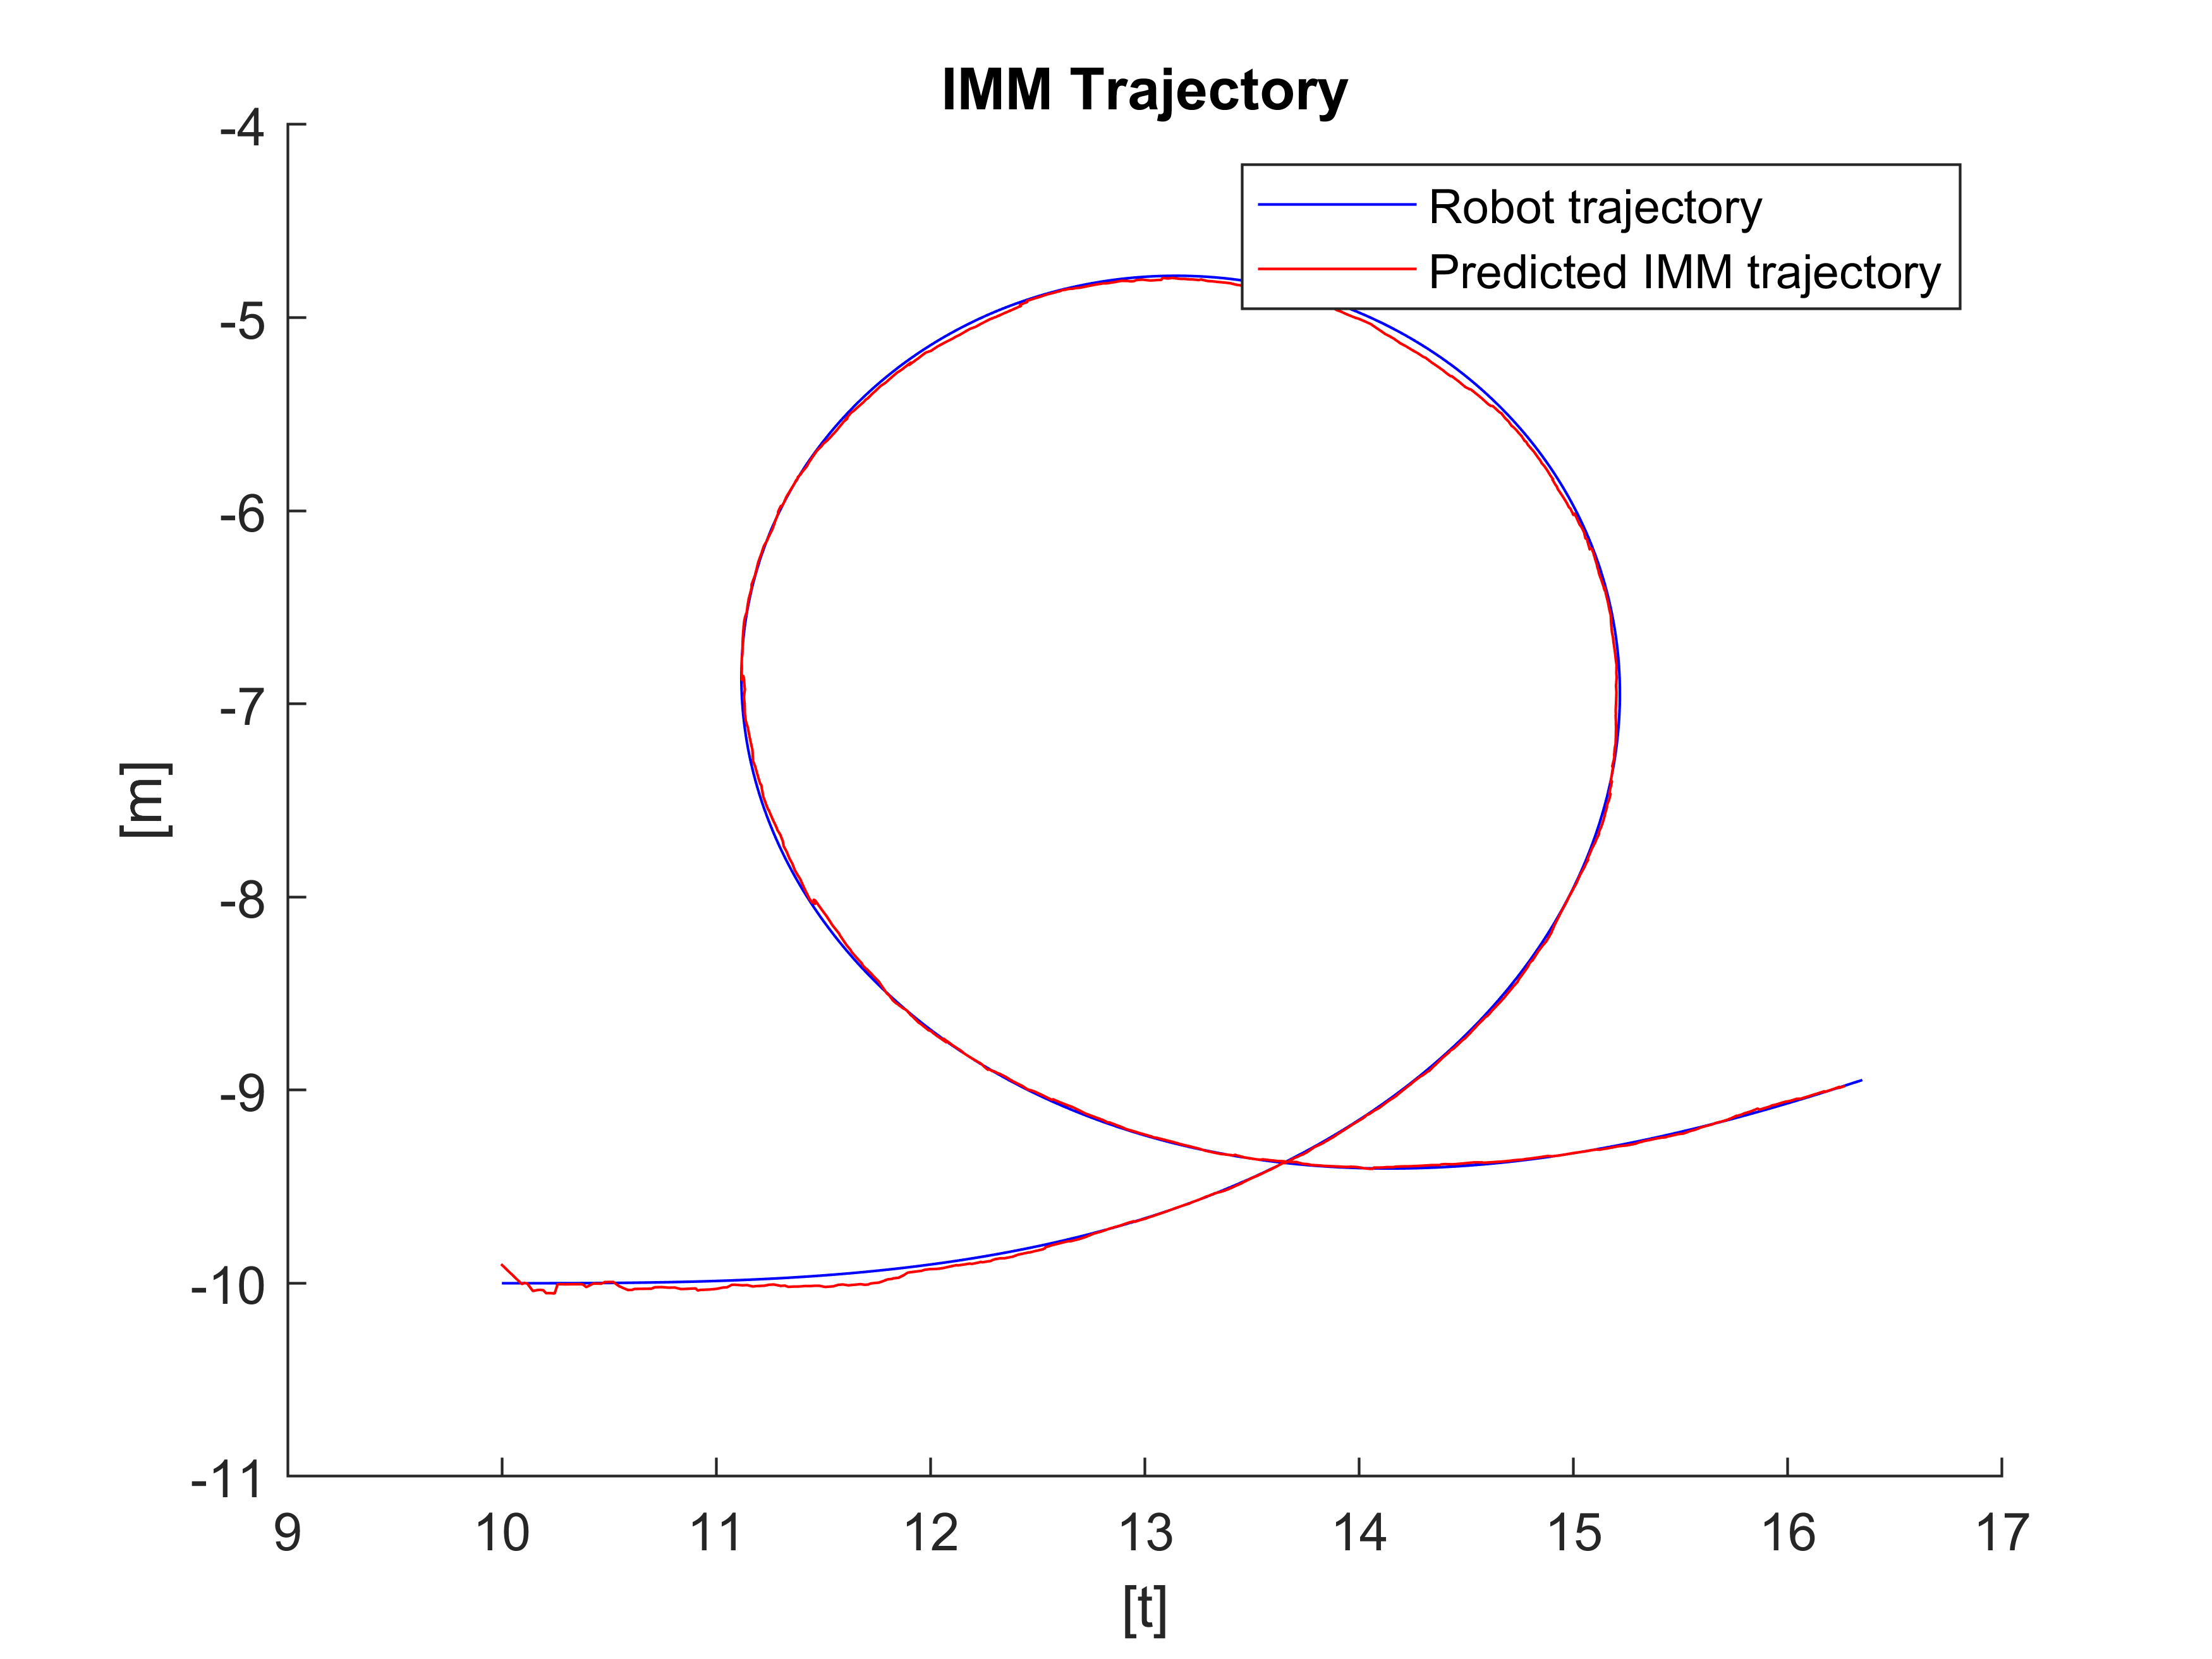
\includegraphics[width=\linewidth]{dwg/IMM-trj.png}
  \caption{IMM Trajectory vs Robot Trajectory}
  \label{fig:second}
\end{figure}

From figure 6 to figure 9 it is possible to assess that the results for the simple implementation of the EKF.

\begin{figure}[H]
 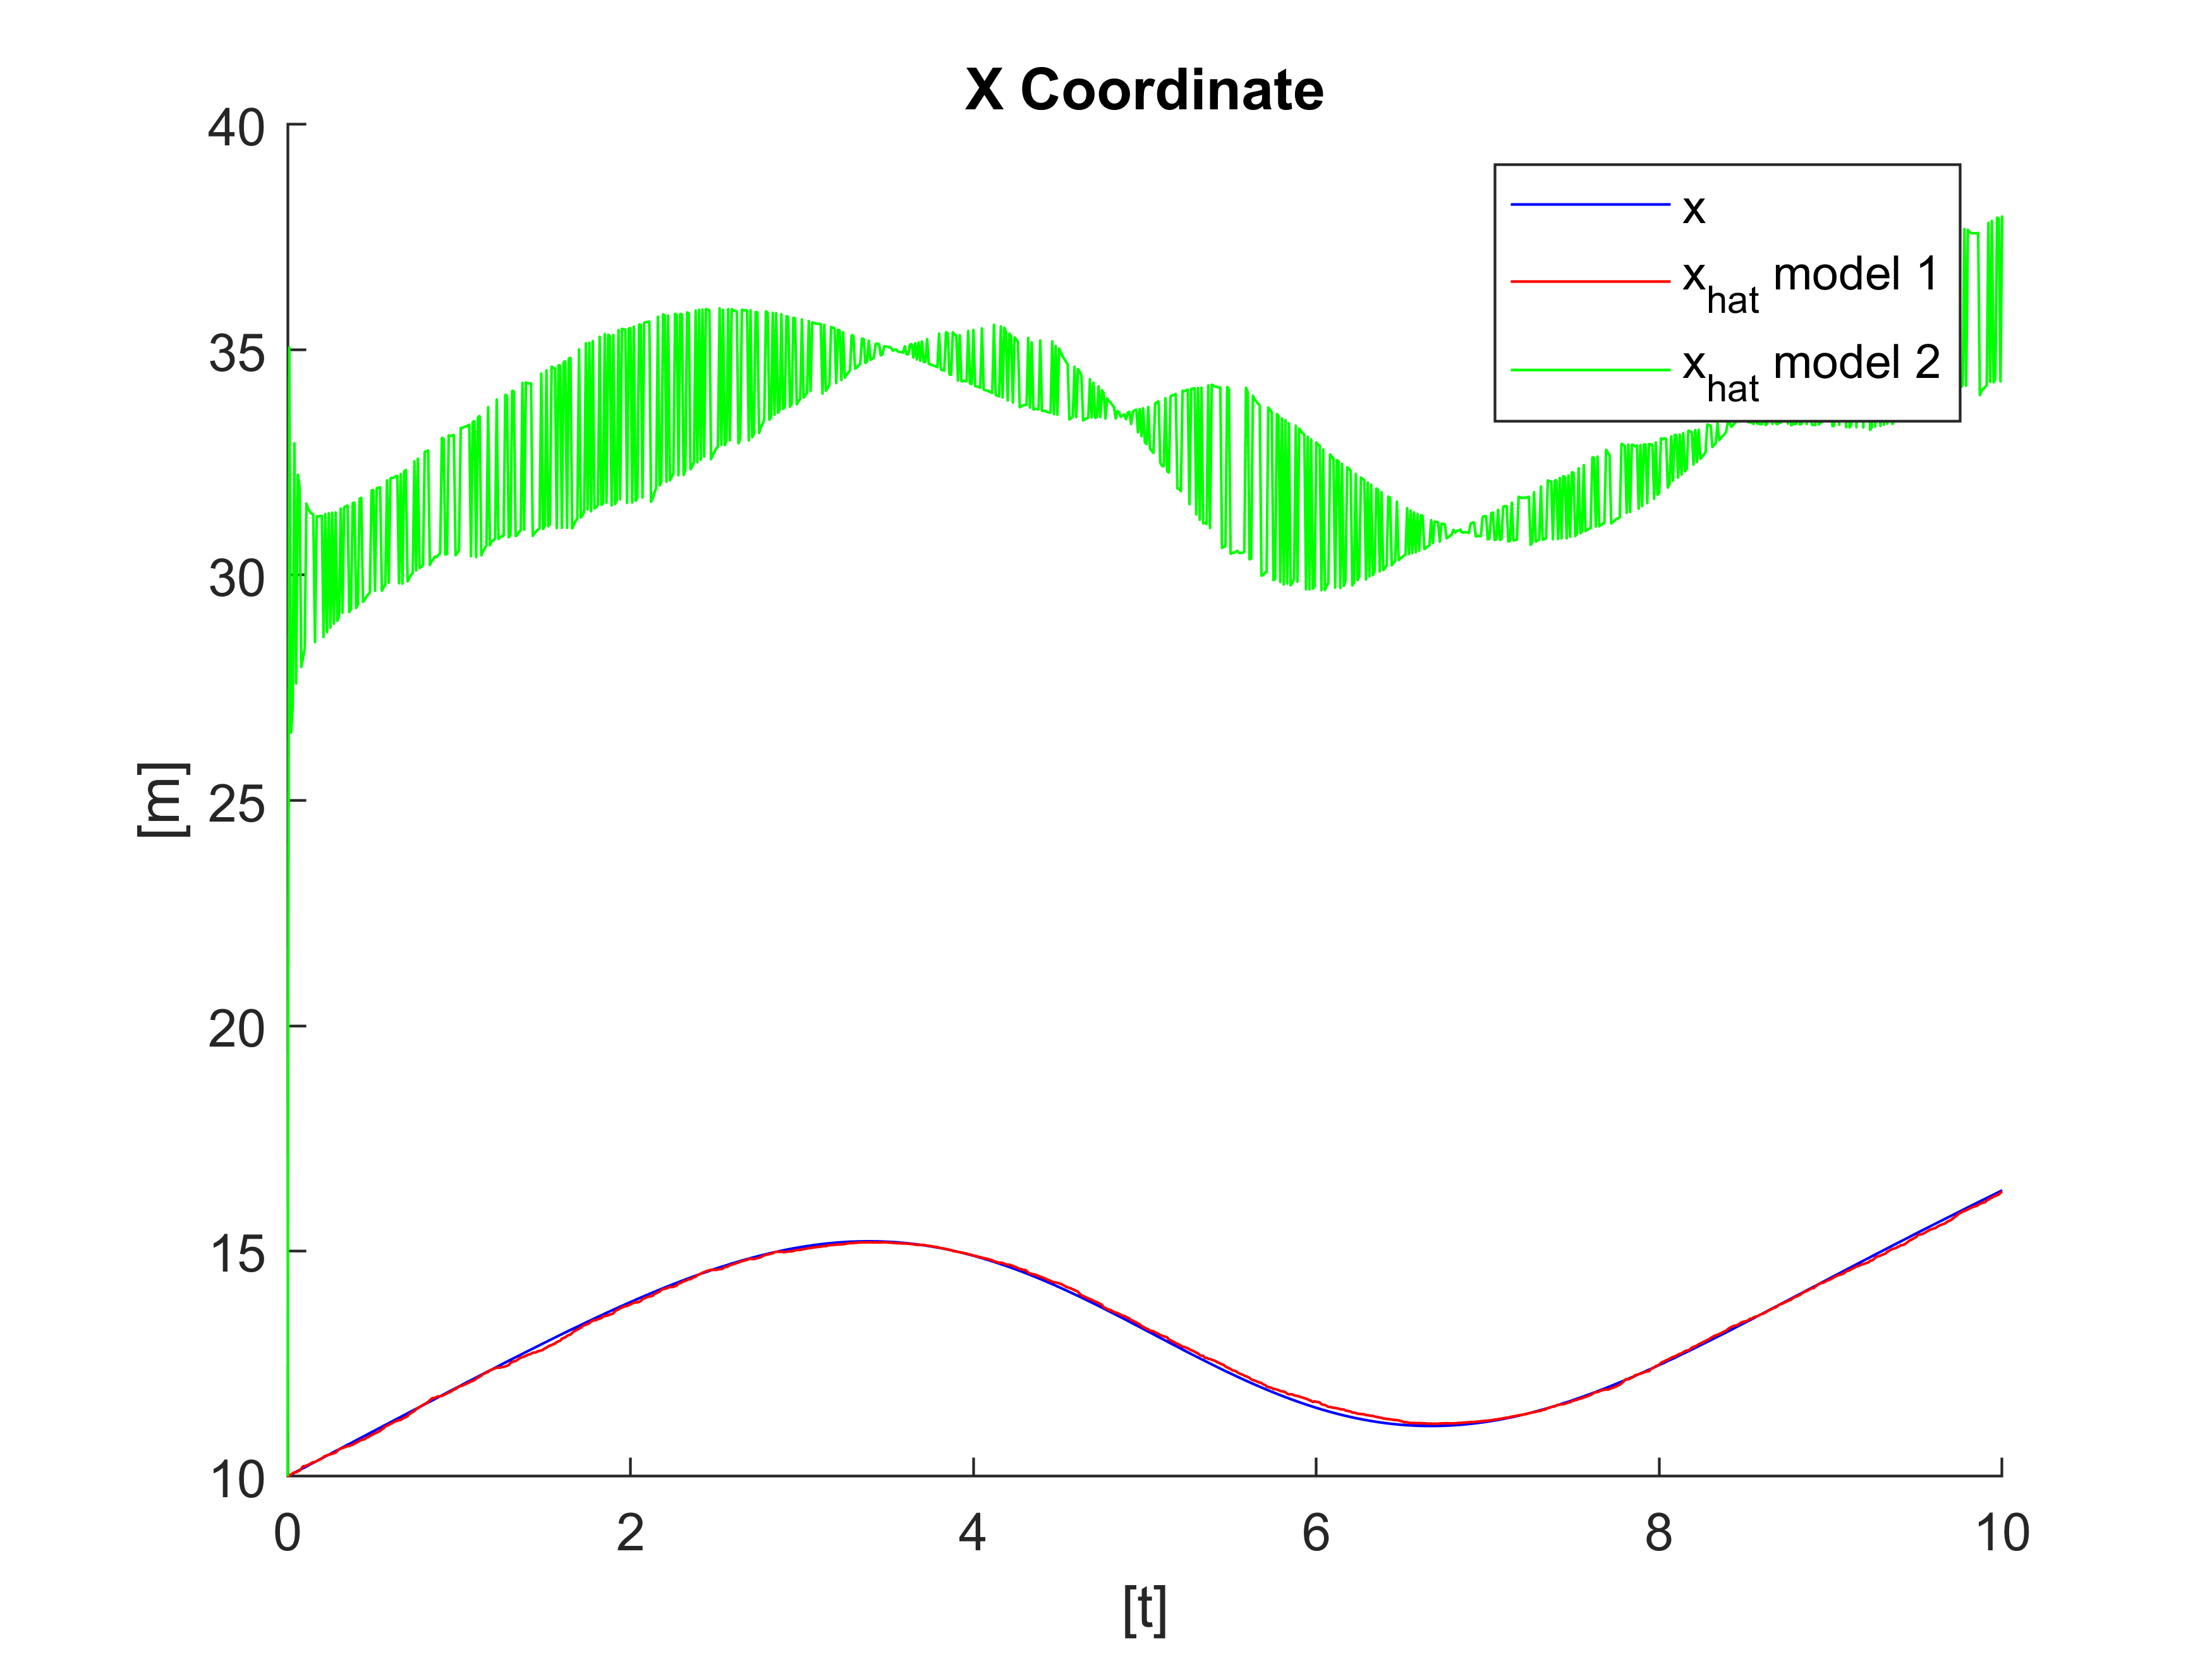
\includegraphics[width=\linewidth]{dwg/centralized-x-coord.png}
  \caption{Centralized EKF - X coordinates}
 
\end{figure}

\begin{figure}[H]
 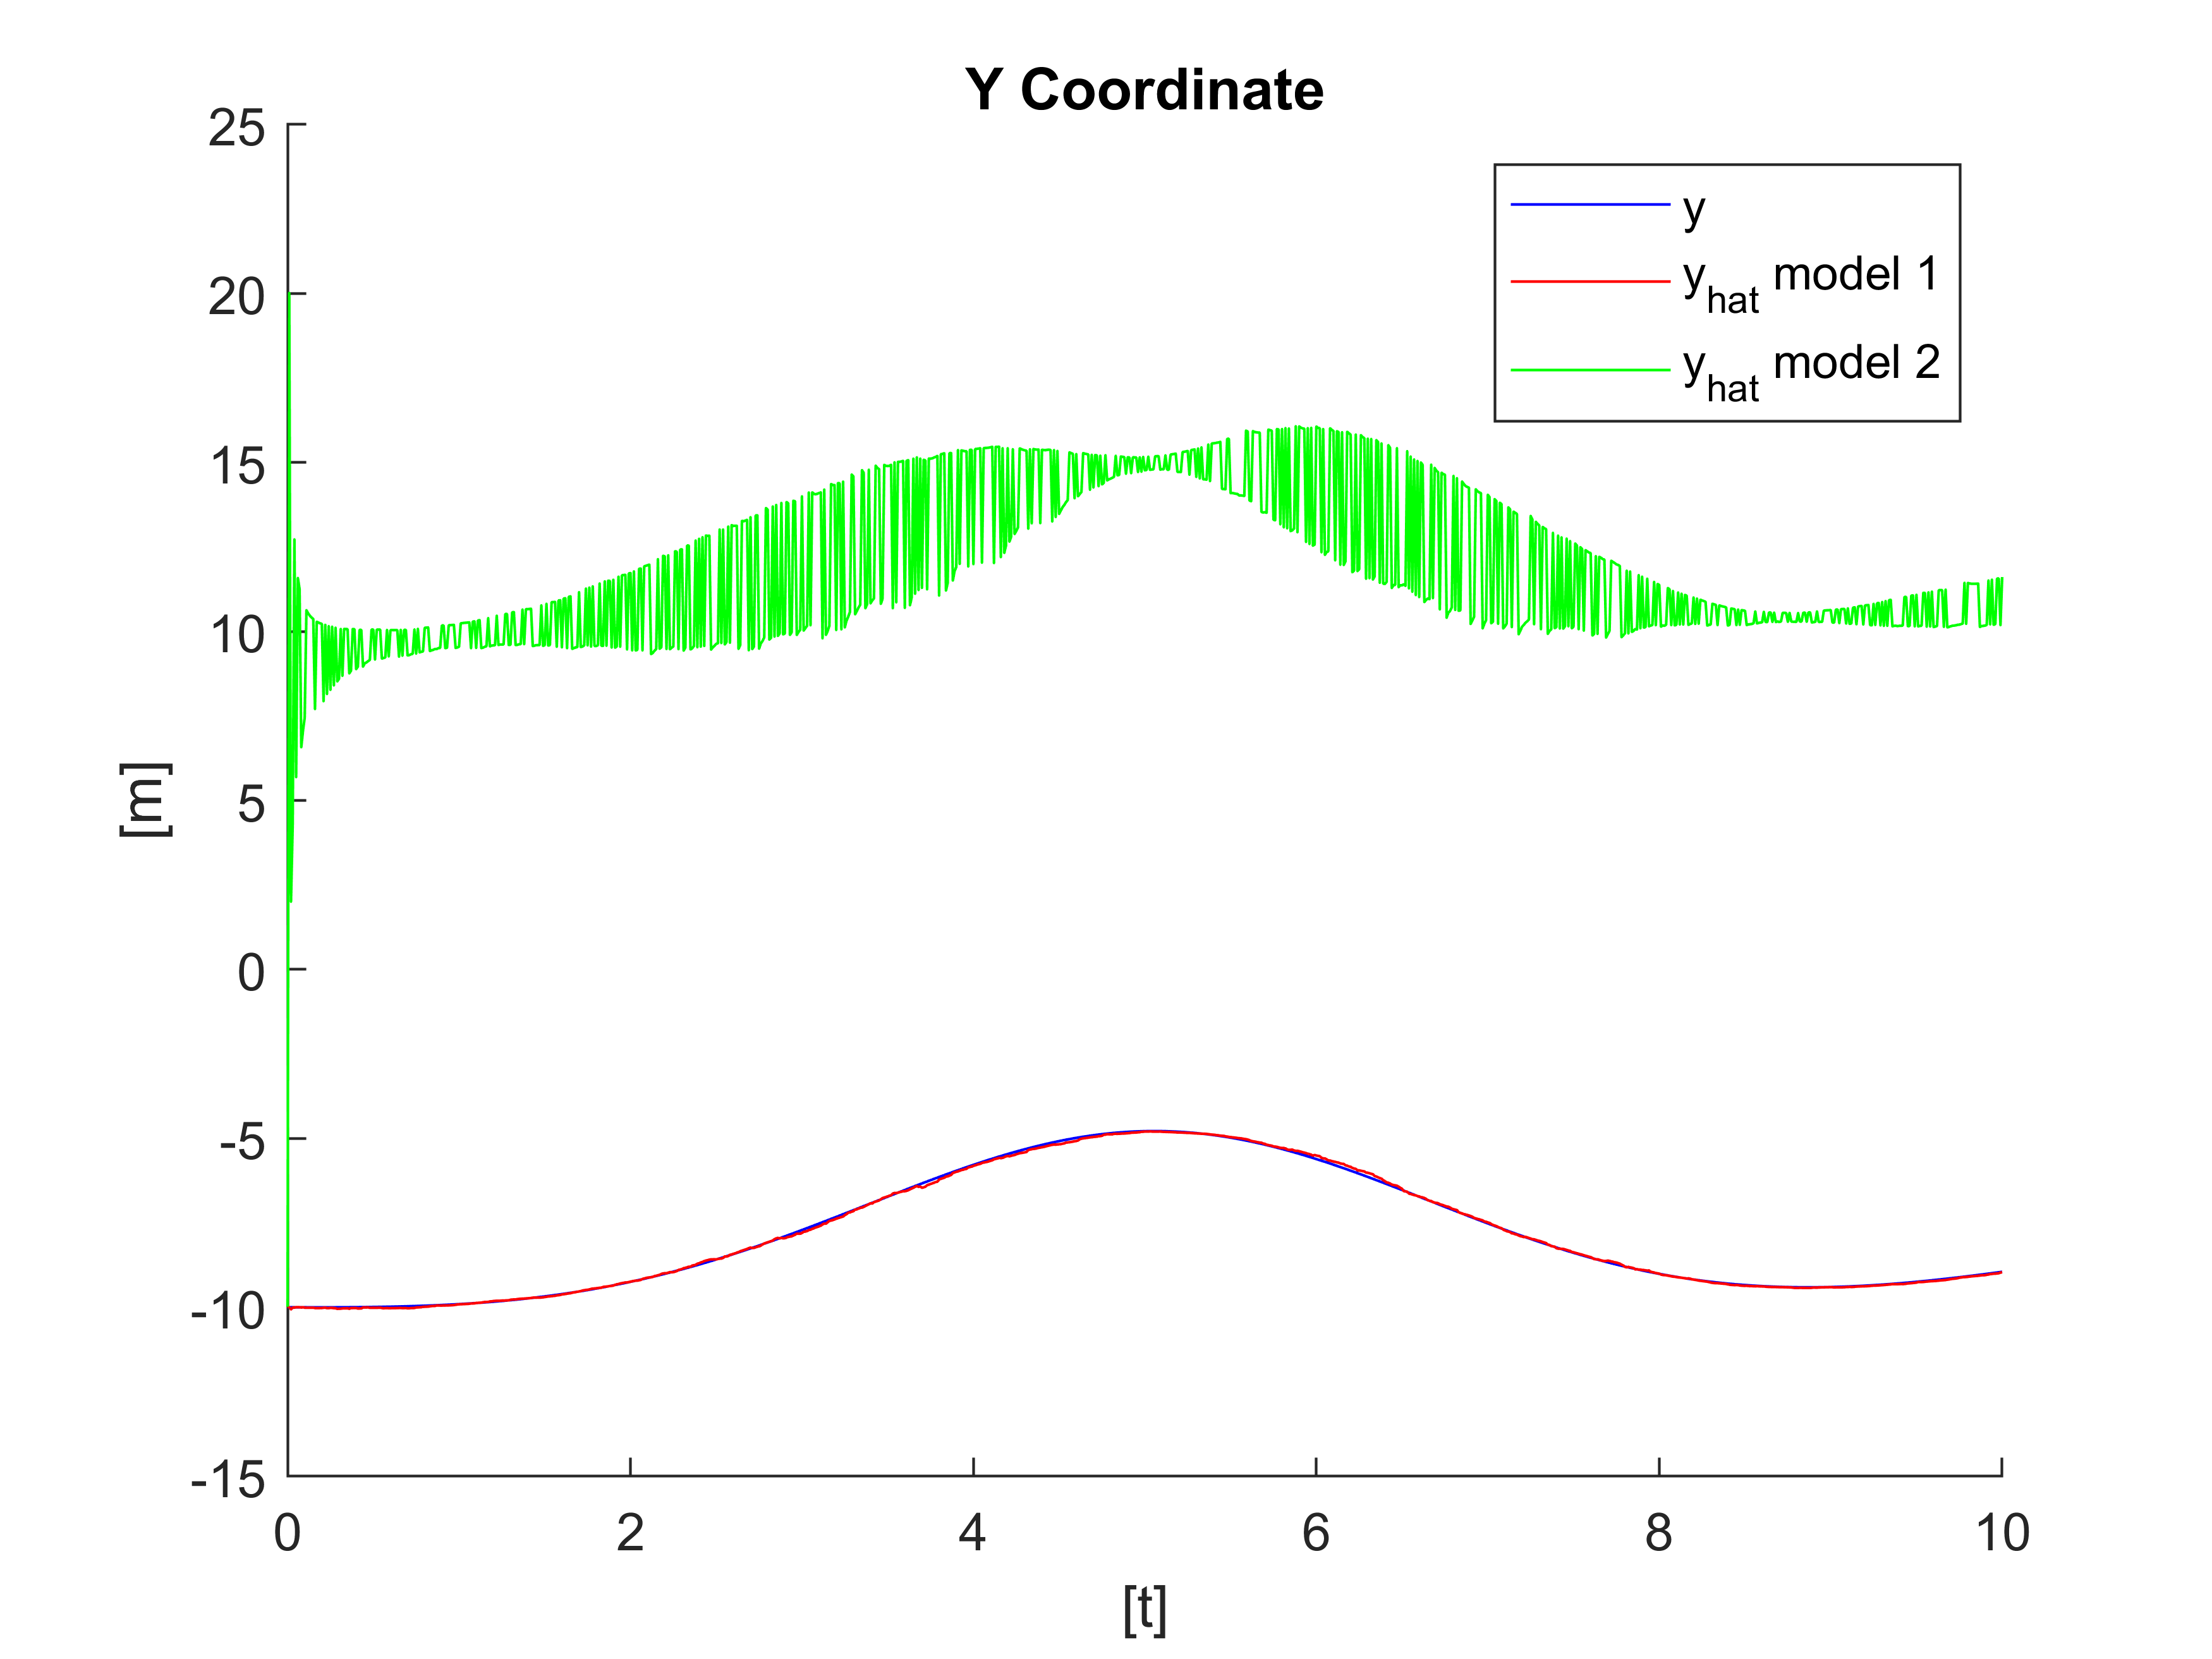
\includegraphics[width=\linewidth]{dwg/centralized-y-coord.png}
  \caption{Centralized EKF - Y coordinates}
 
\end{figure}

\begin{figure}[H]
 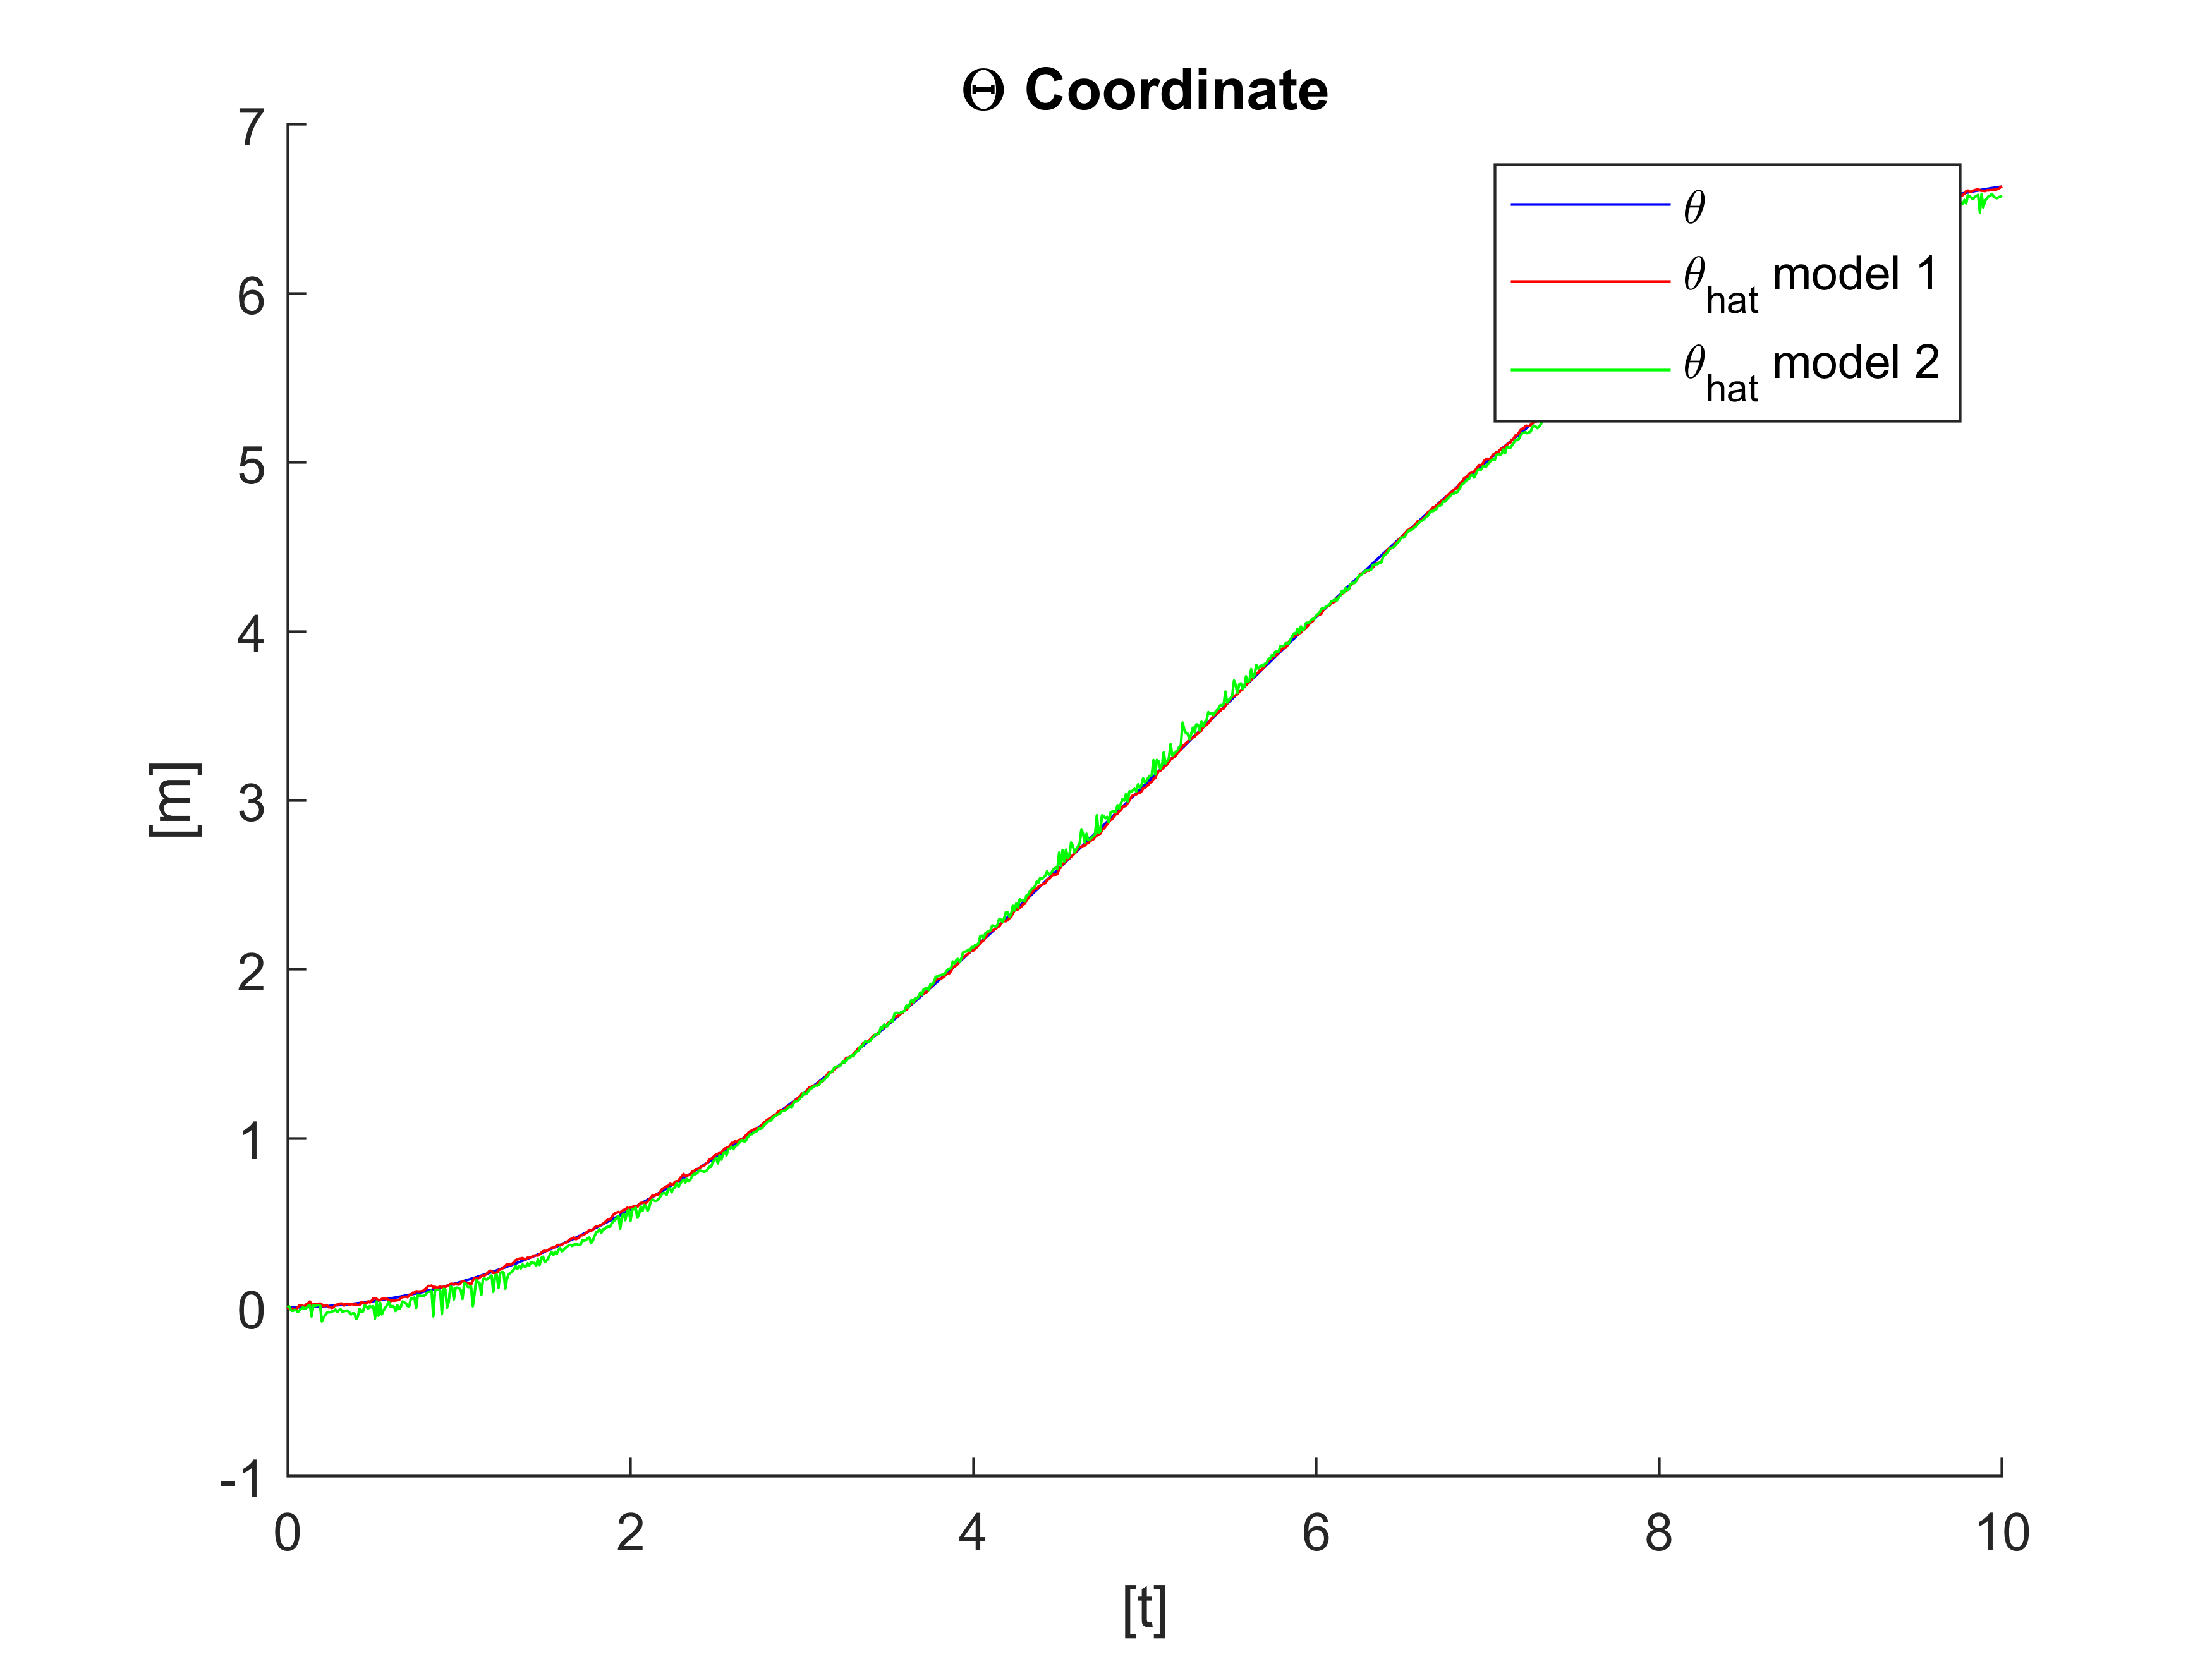
\includegraphics[width=\linewidth]{dwg/centralized-t-coord.png}
  \caption{Centralized EKF - $\Theta$ coordinates}
 
\end{figure}


\bigskip \bigskip \bigskip \bigskip \bigskip \bigskip \bigskip \bigskip \bigskip \bigskip \bigskip \bigskip \bigskip \bigskip \bigskip \bigskip 
\begin{figure}[H]
 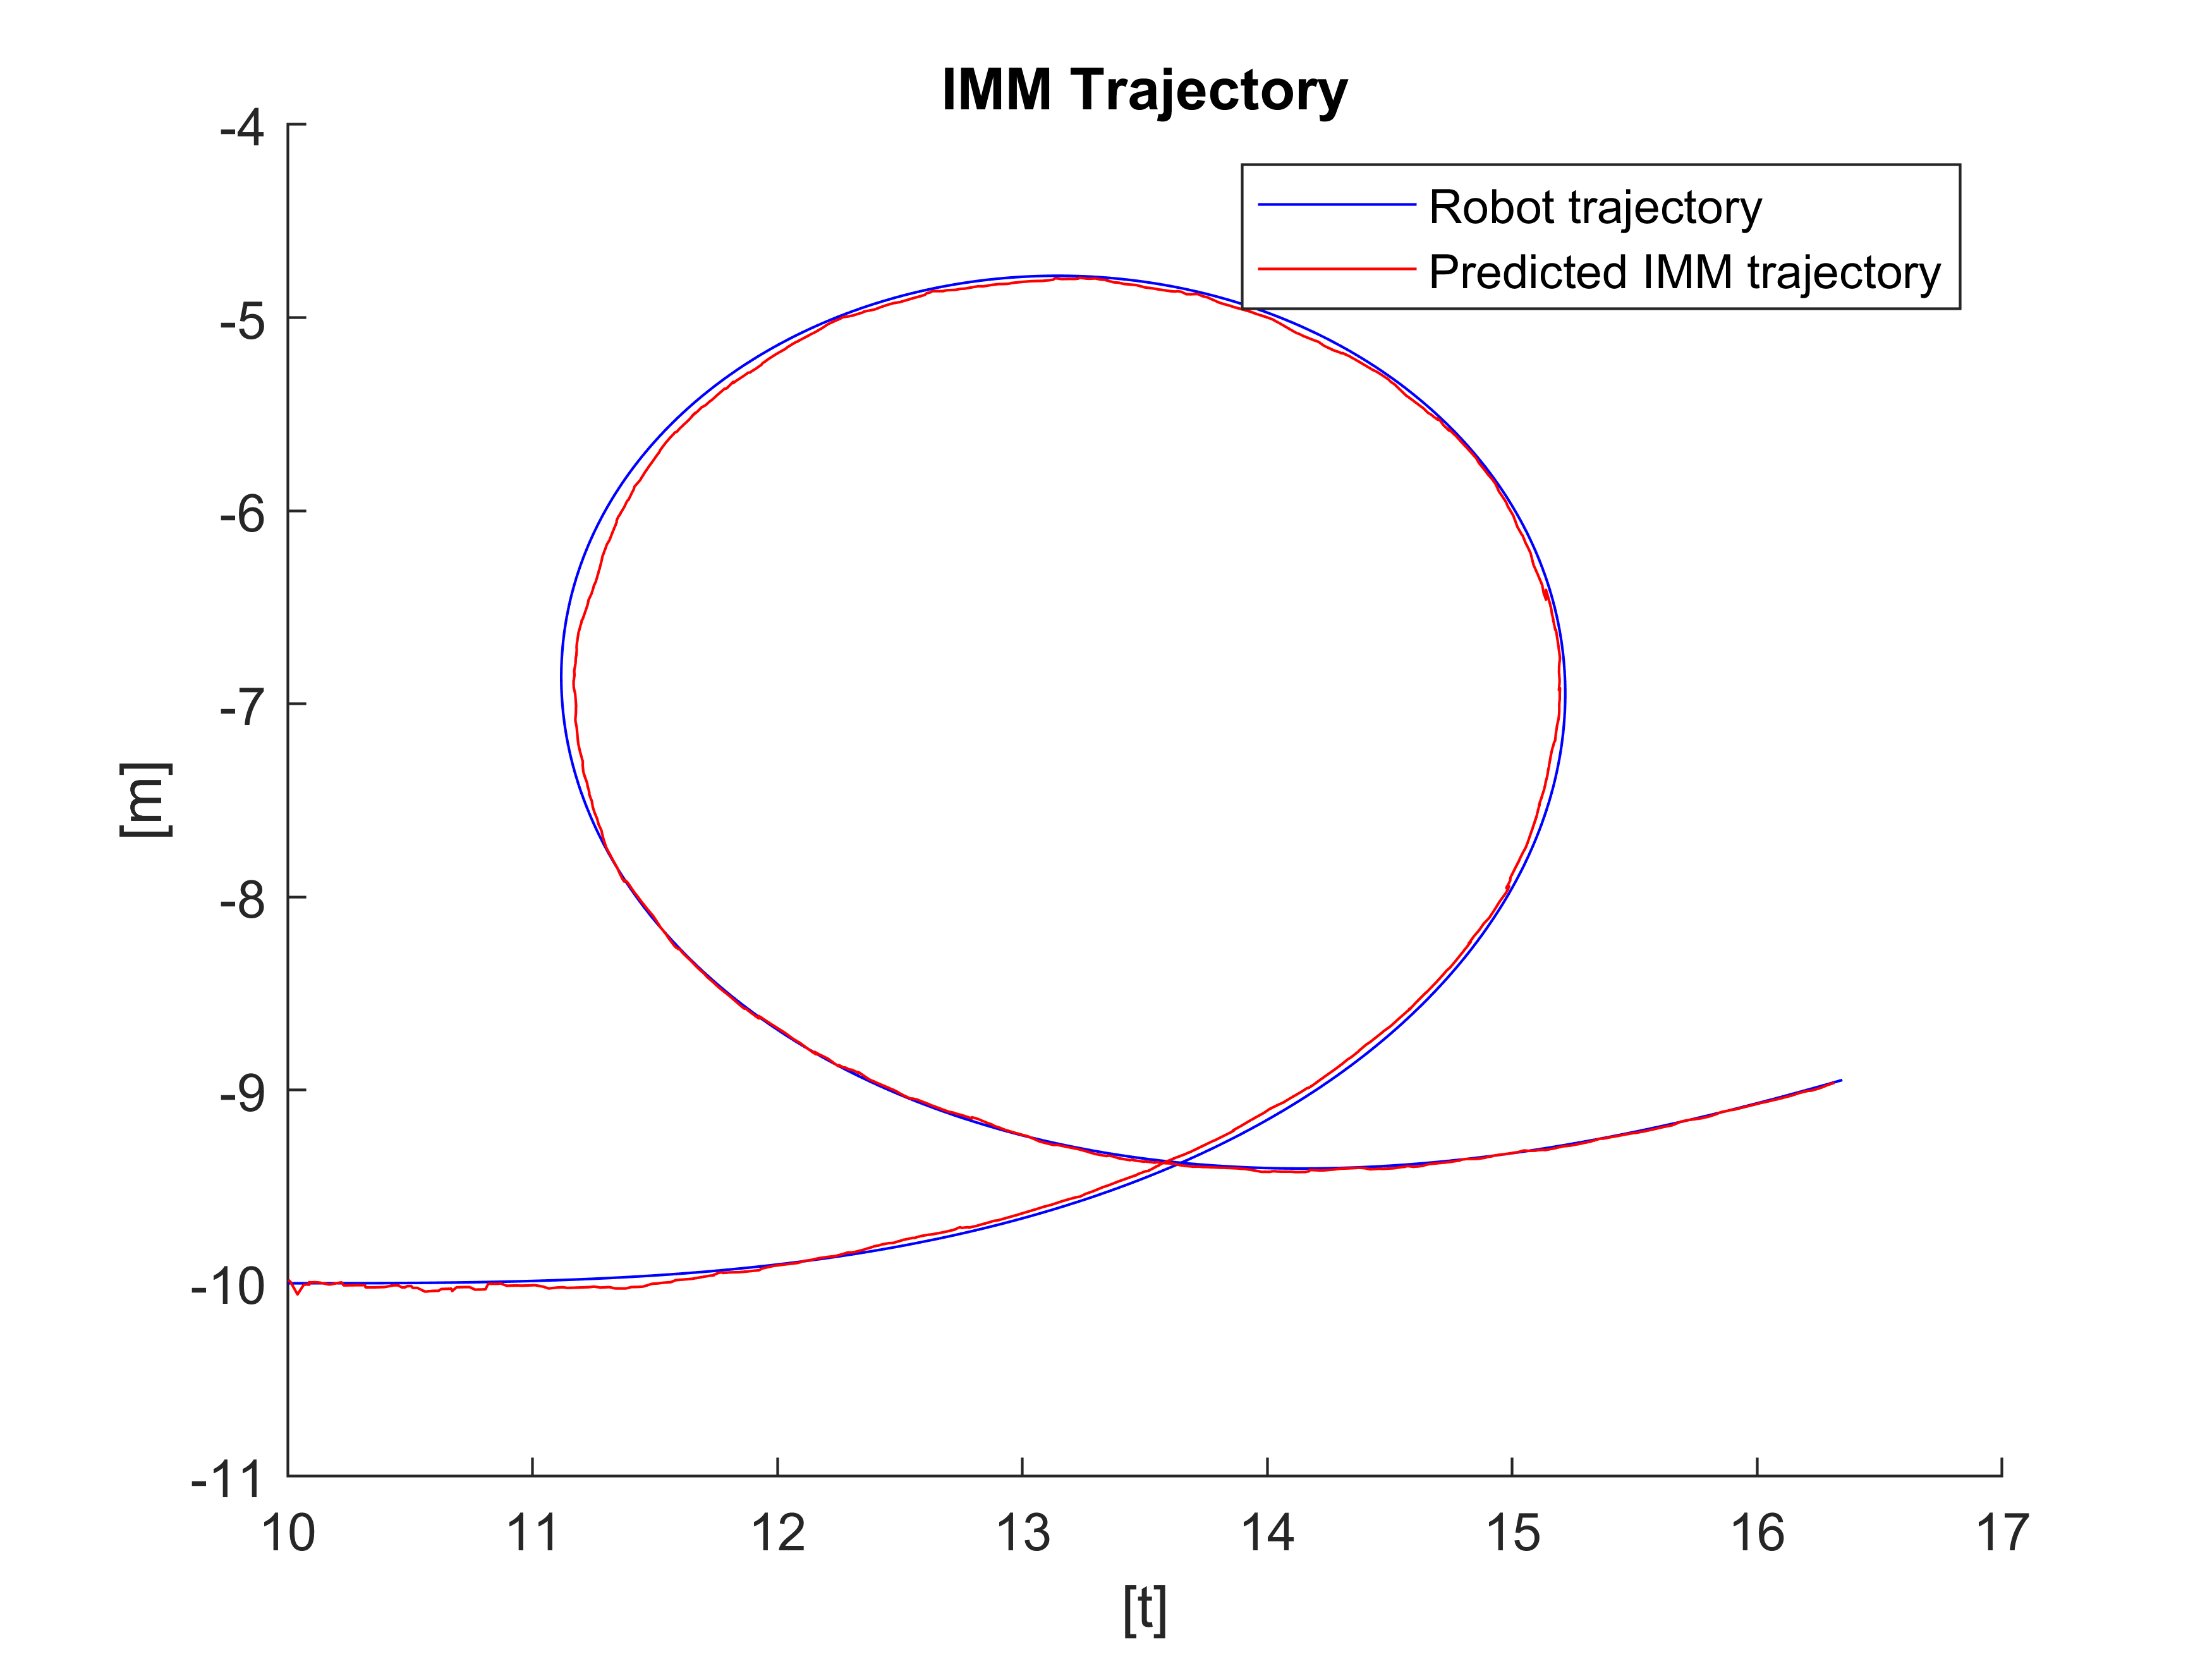
\includegraphics[width=\linewidth]{dwg/Centralized-IMM-trj.png}
  \caption{Centralized IMM Trajectory vs Robot Trajectory}
 
\end{figure}

\bigskip \bigskip \bigskip \bigskip \bigskip \bigskip \bigskip \bigskip \bigskip \bigskip \bigskip \bigskip \bigskip \bigskip \bigskip \bigskip \bigskip \bigskip \bigskip \bigskip \bigskip \bigskip \bigskip \bigskip \bigskip \bigskip \bigskip \bigskip
 While from figure 10 to figure 13 the results of the centralized implementation are shown. It can be seen that the plots are basically the same but to have a deeper insight on this we will now plot the error that the IMM estimator have with respect to the real state of the robot for each of the Kalman Filter version. Since Kalman Filter is known to be a MMSE Filter we will use a quadratic form to compute the error between real and observed values.

\begin{figure}[H]
 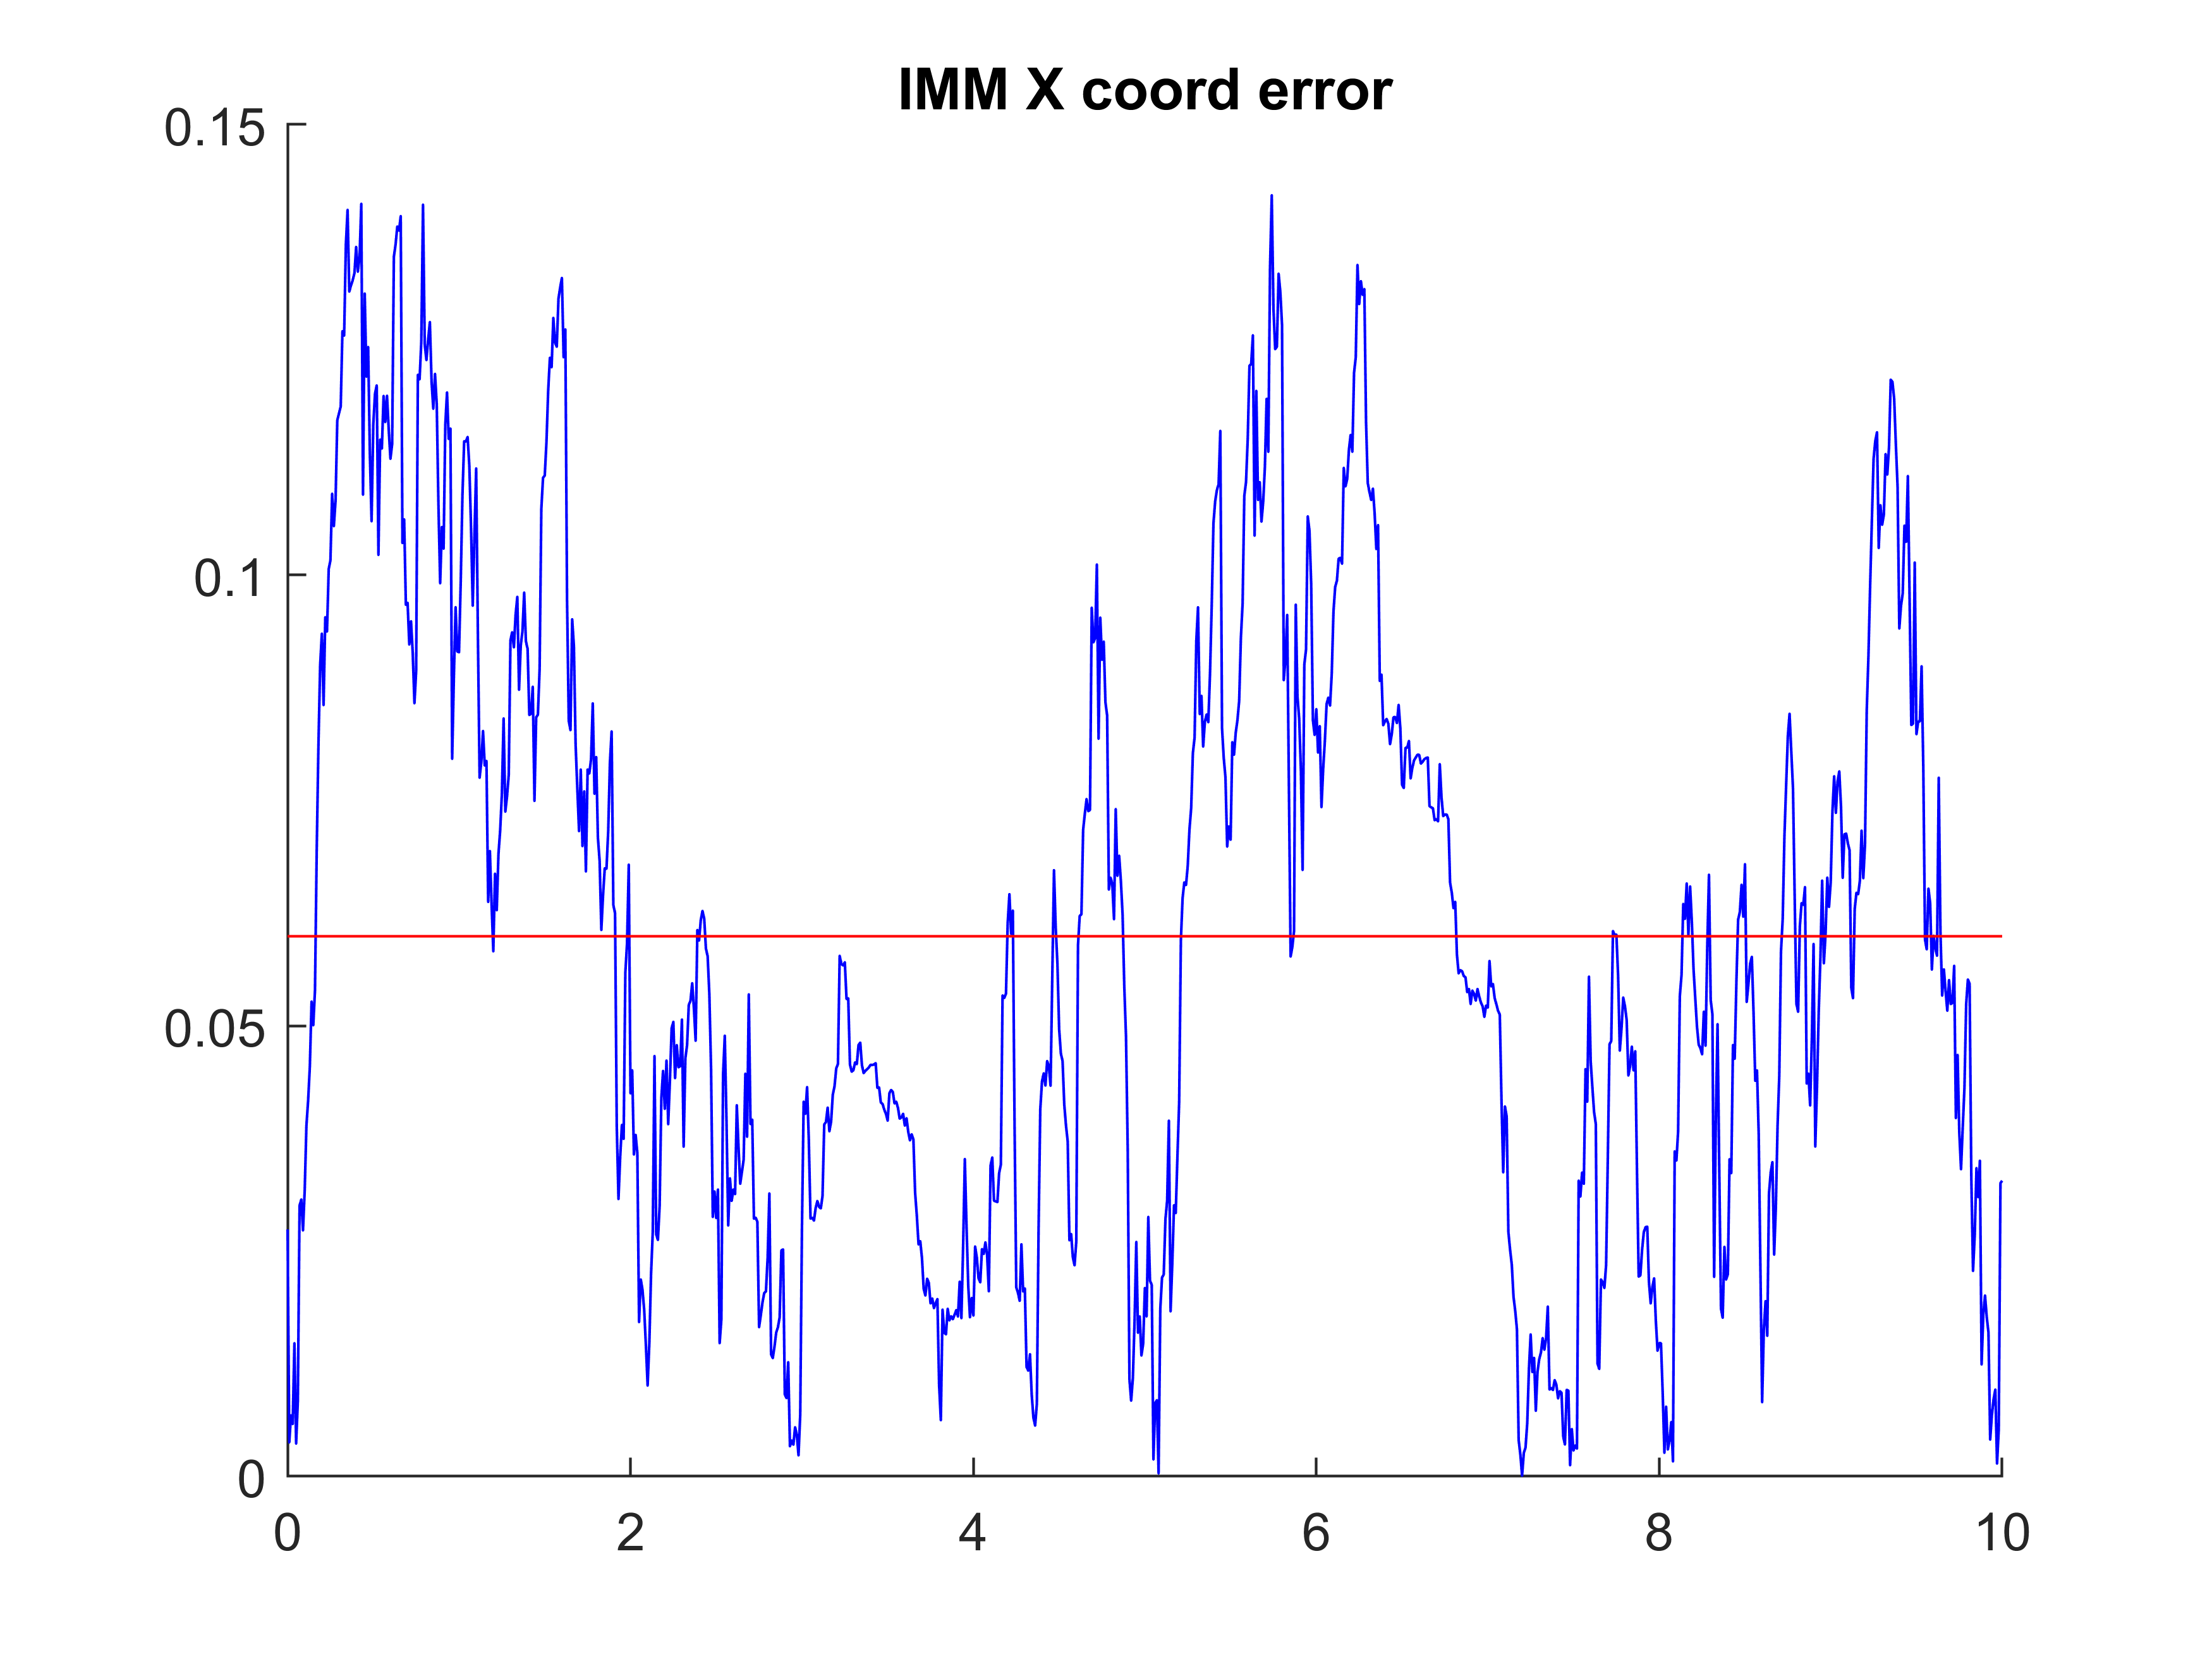
\includegraphics[width=\linewidth]{dwg/IMM-x-error.png}
  \caption{IMM - X Error}
 
\end{figure}

\begin{figure}[H]
 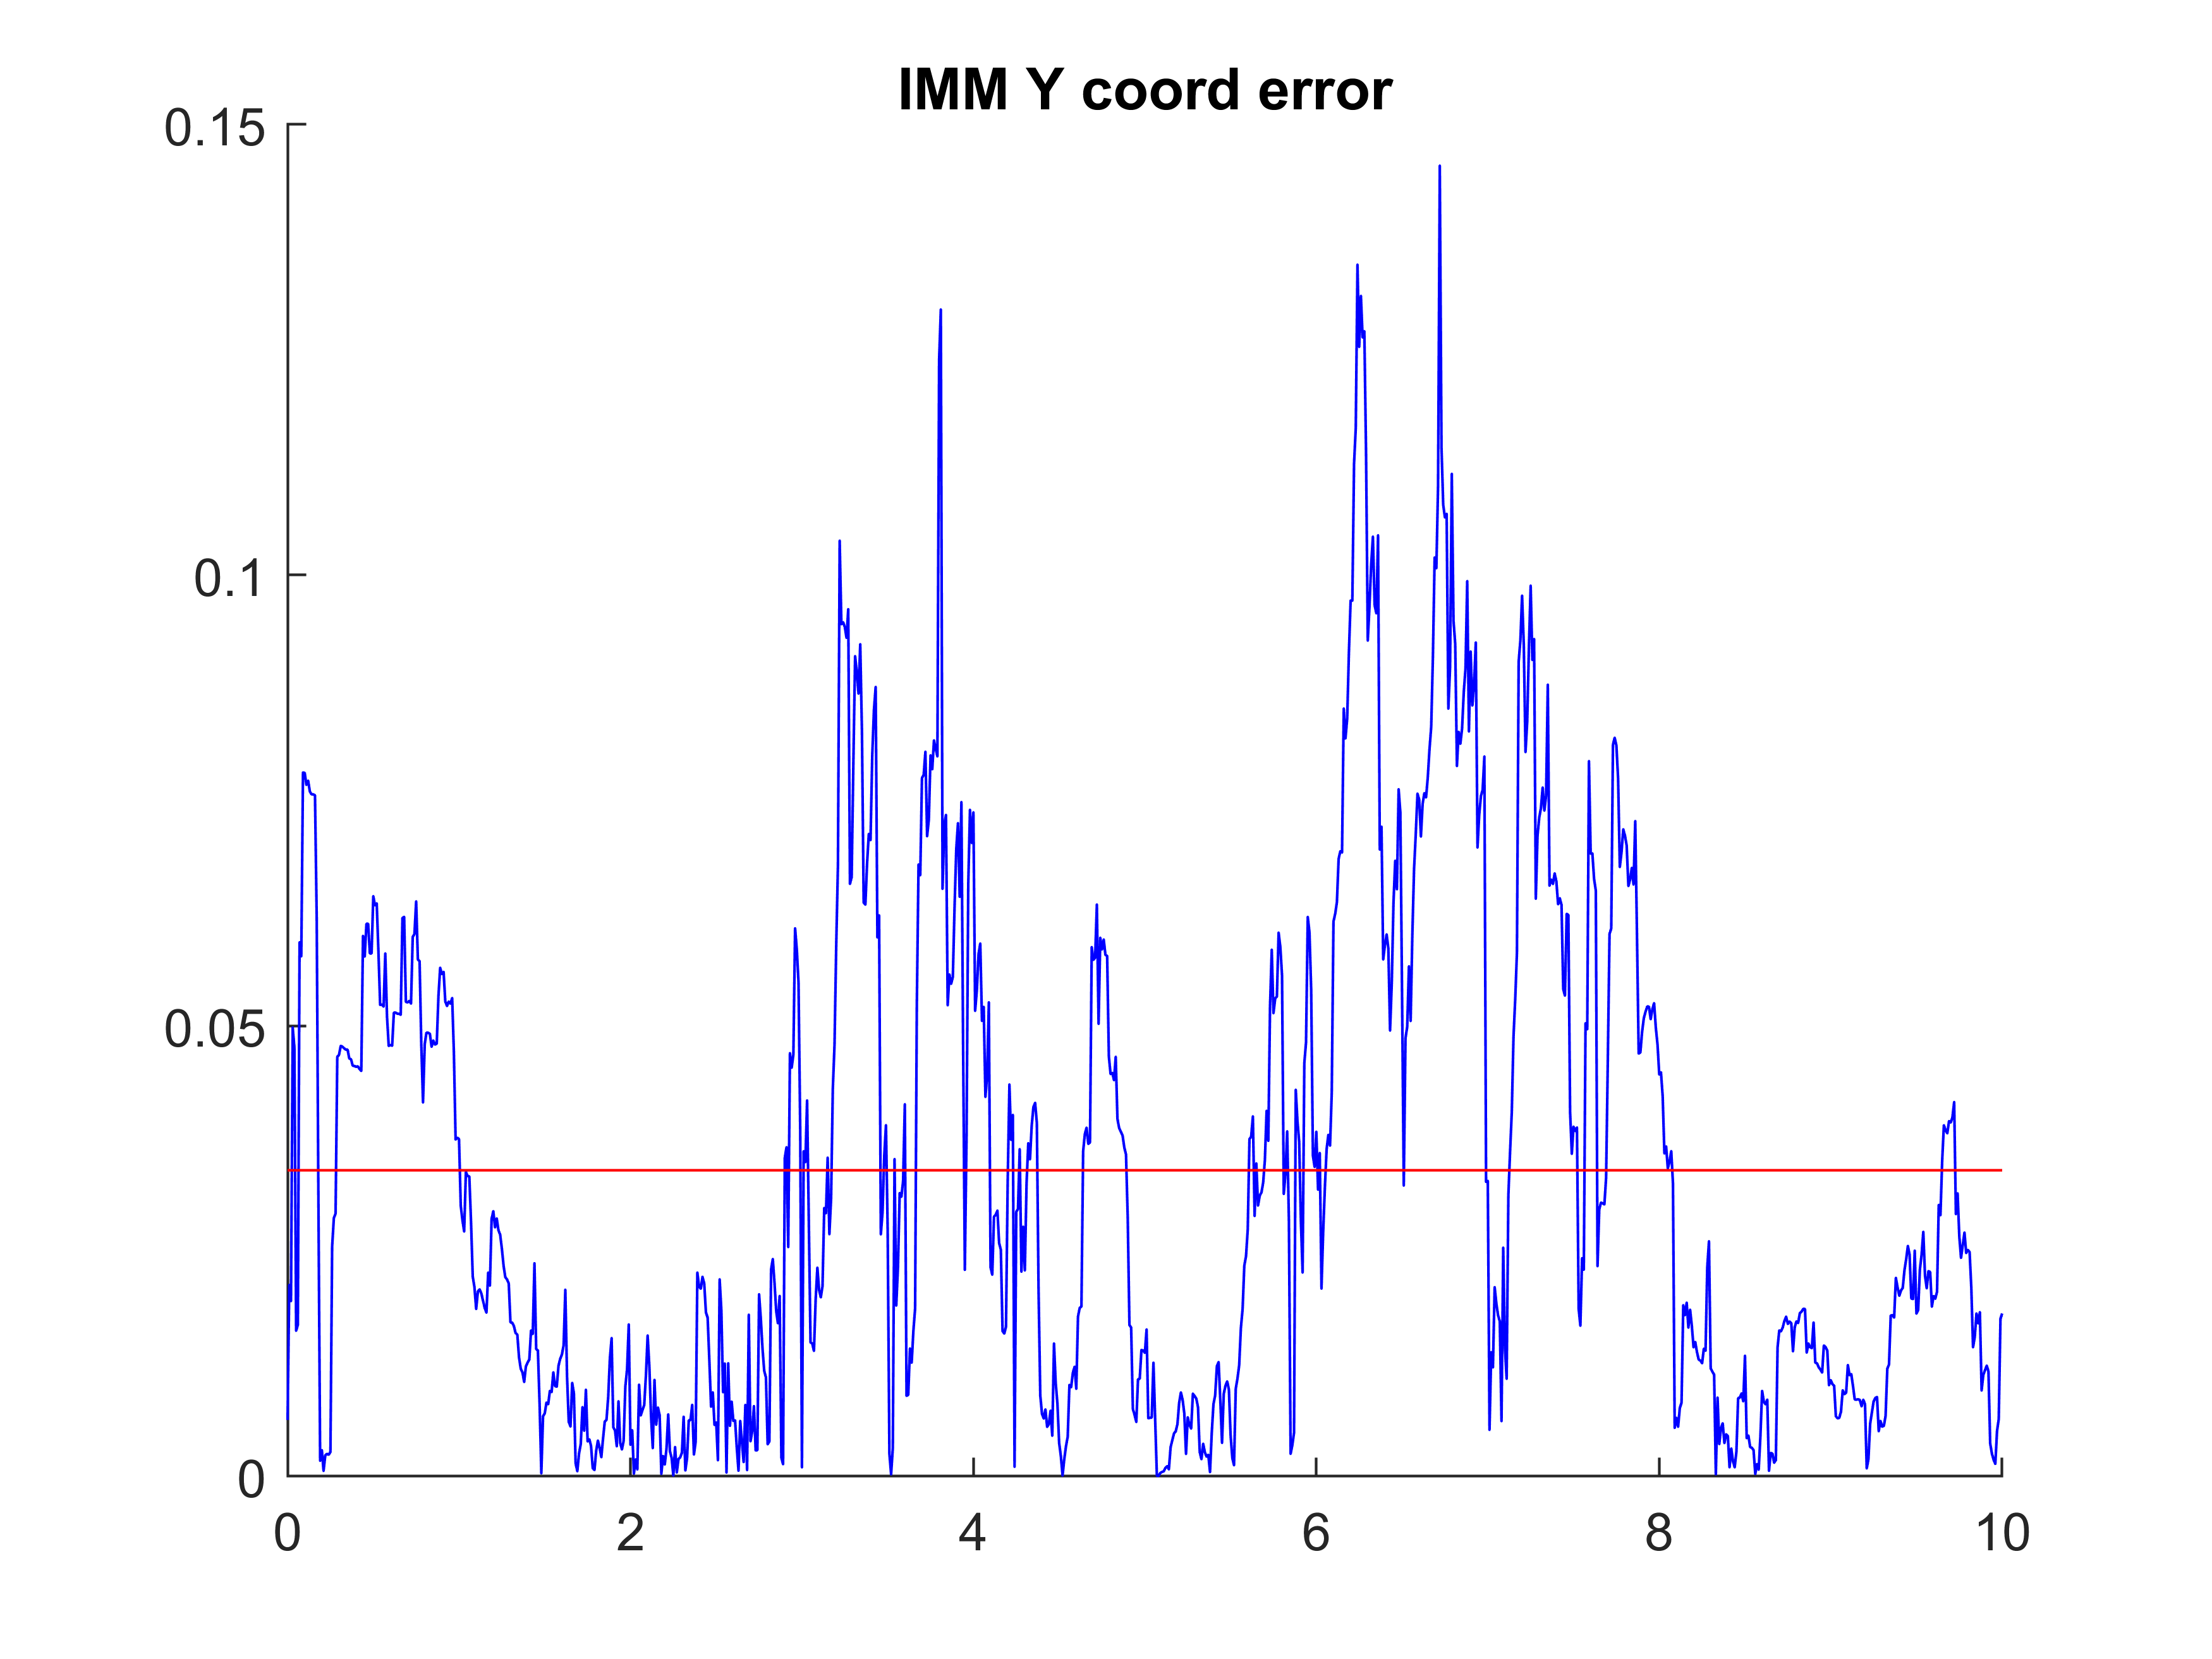
\includegraphics[width=\linewidth]{dwg/IMM-y-error.png}
  \caption{IMM - Y Error}
 
\end{figure}

\begin{figure}[H]
 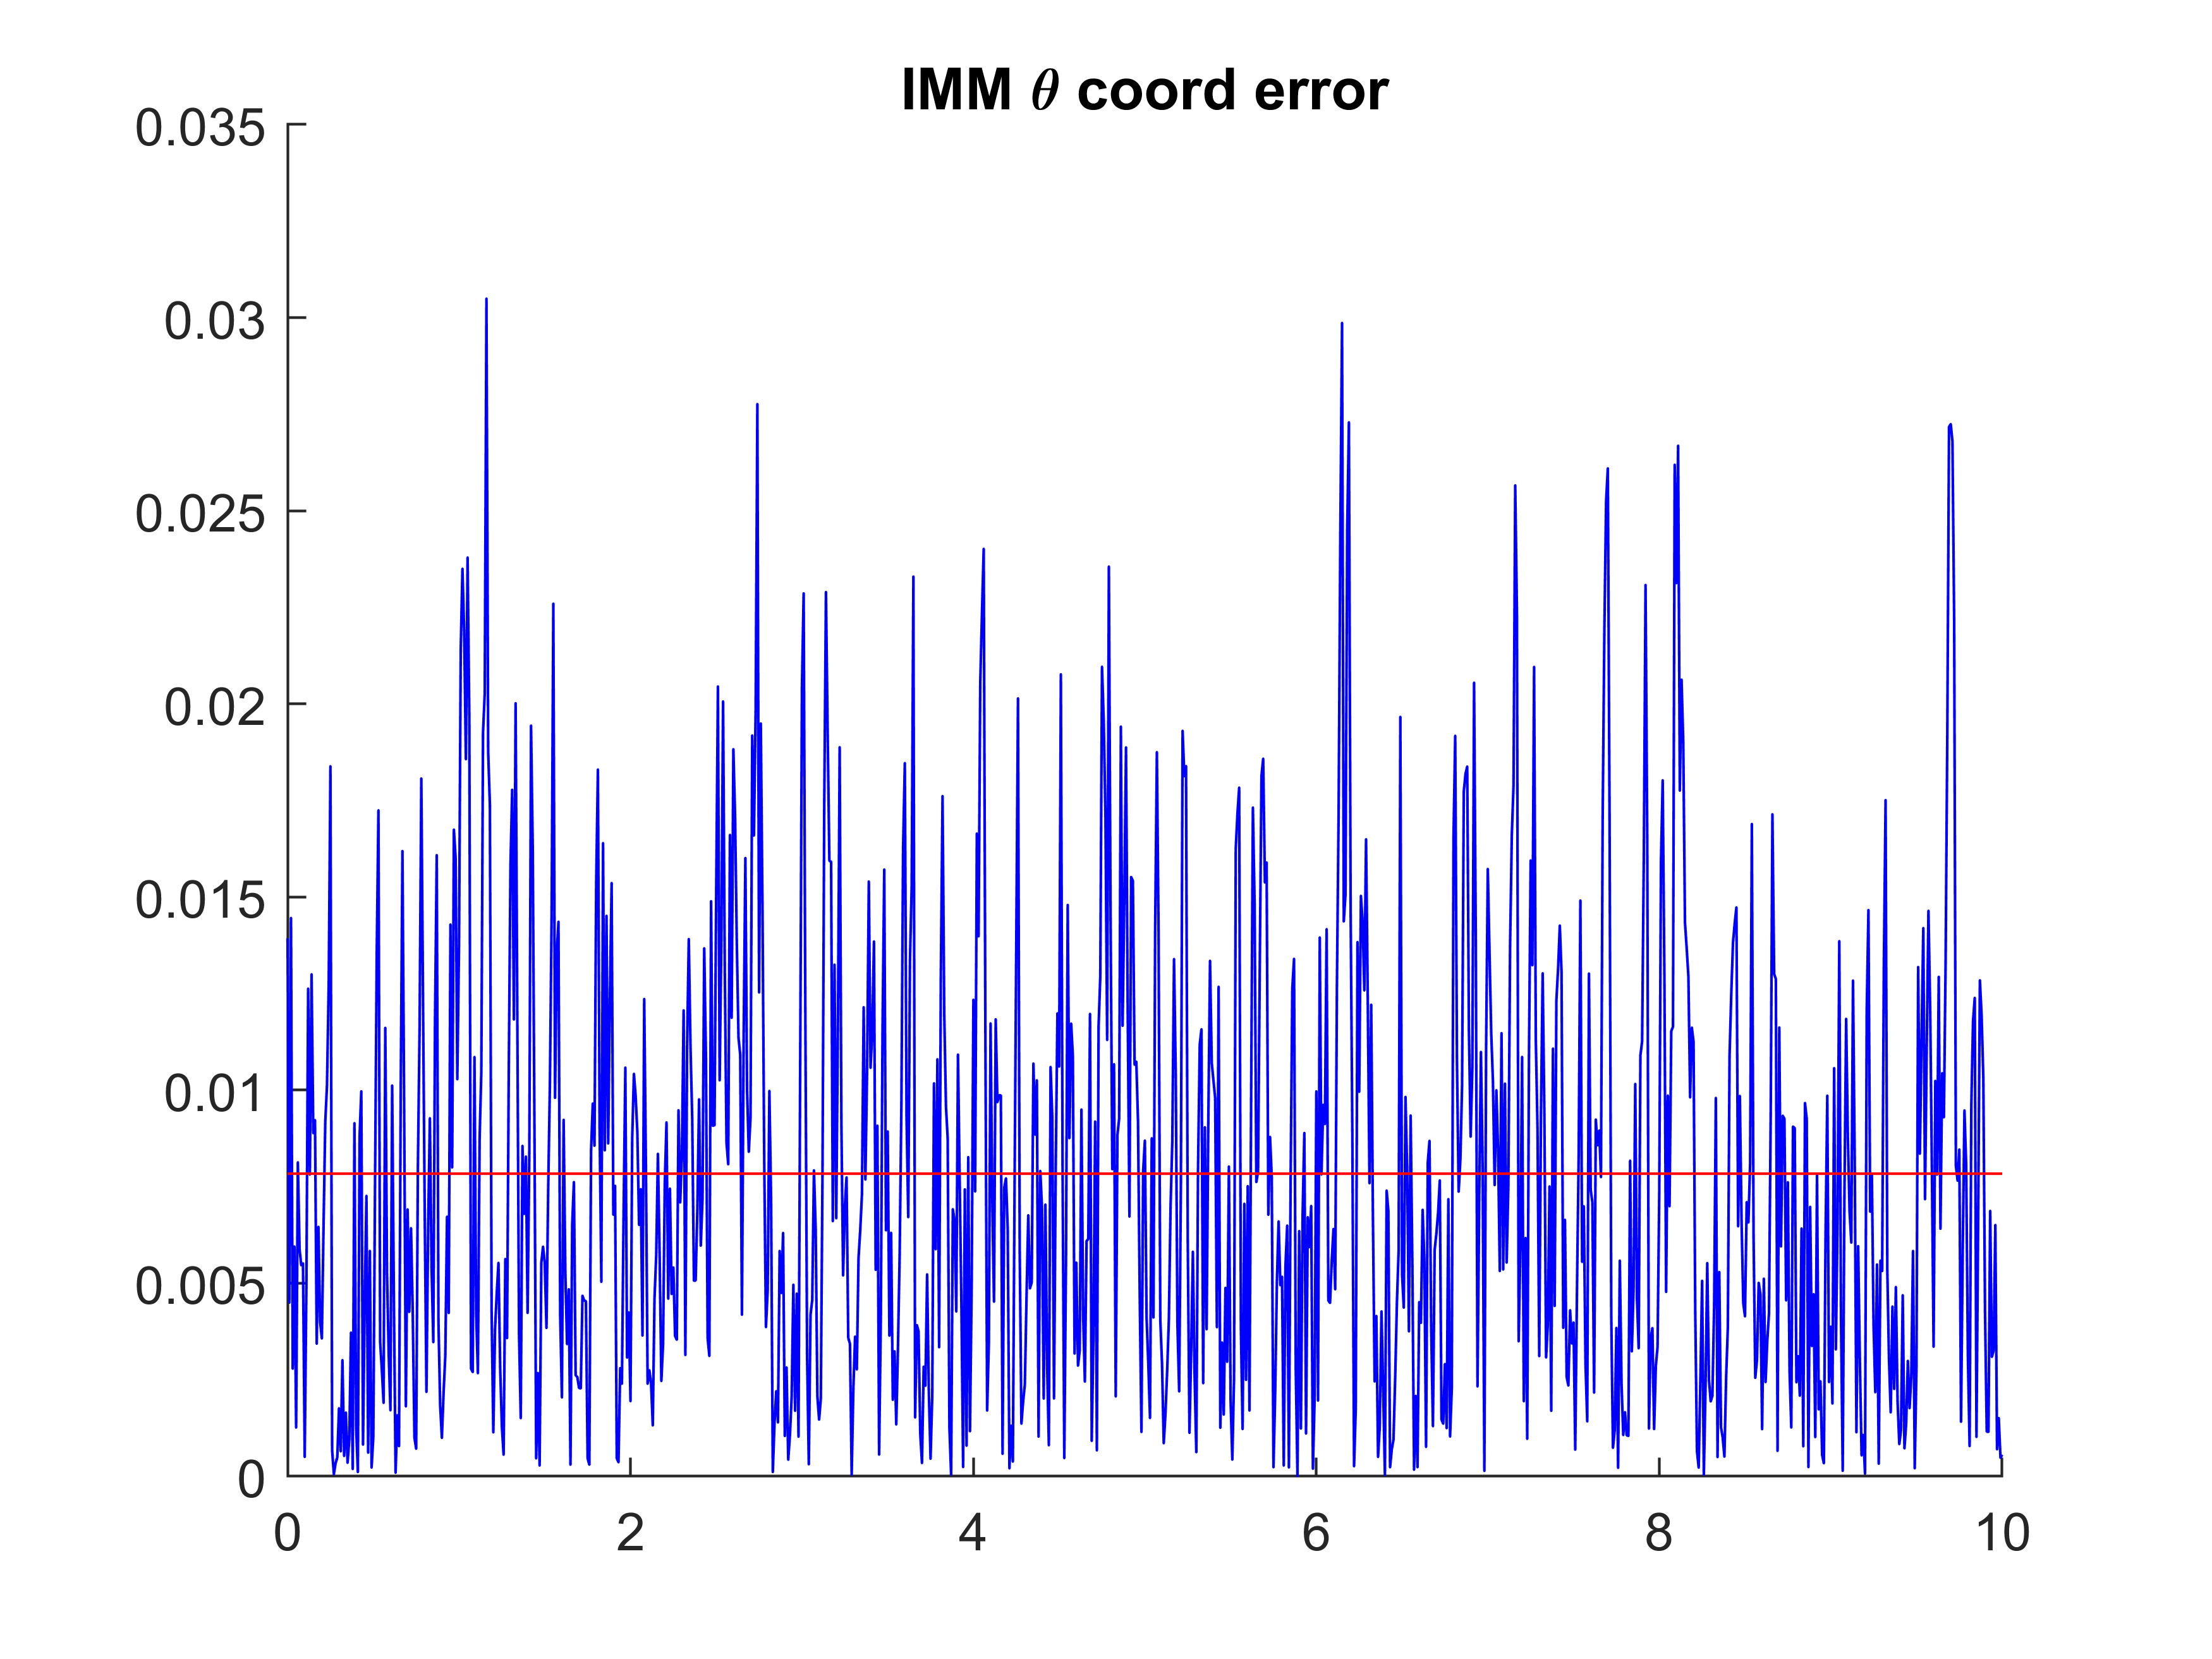
\includegraphics[width=\linewidth]{dwg/IMM-theta-error.png}
  \caption{IMM - $\Theta$ Error}
 
\end{figure}

\begin{figure}[H]
 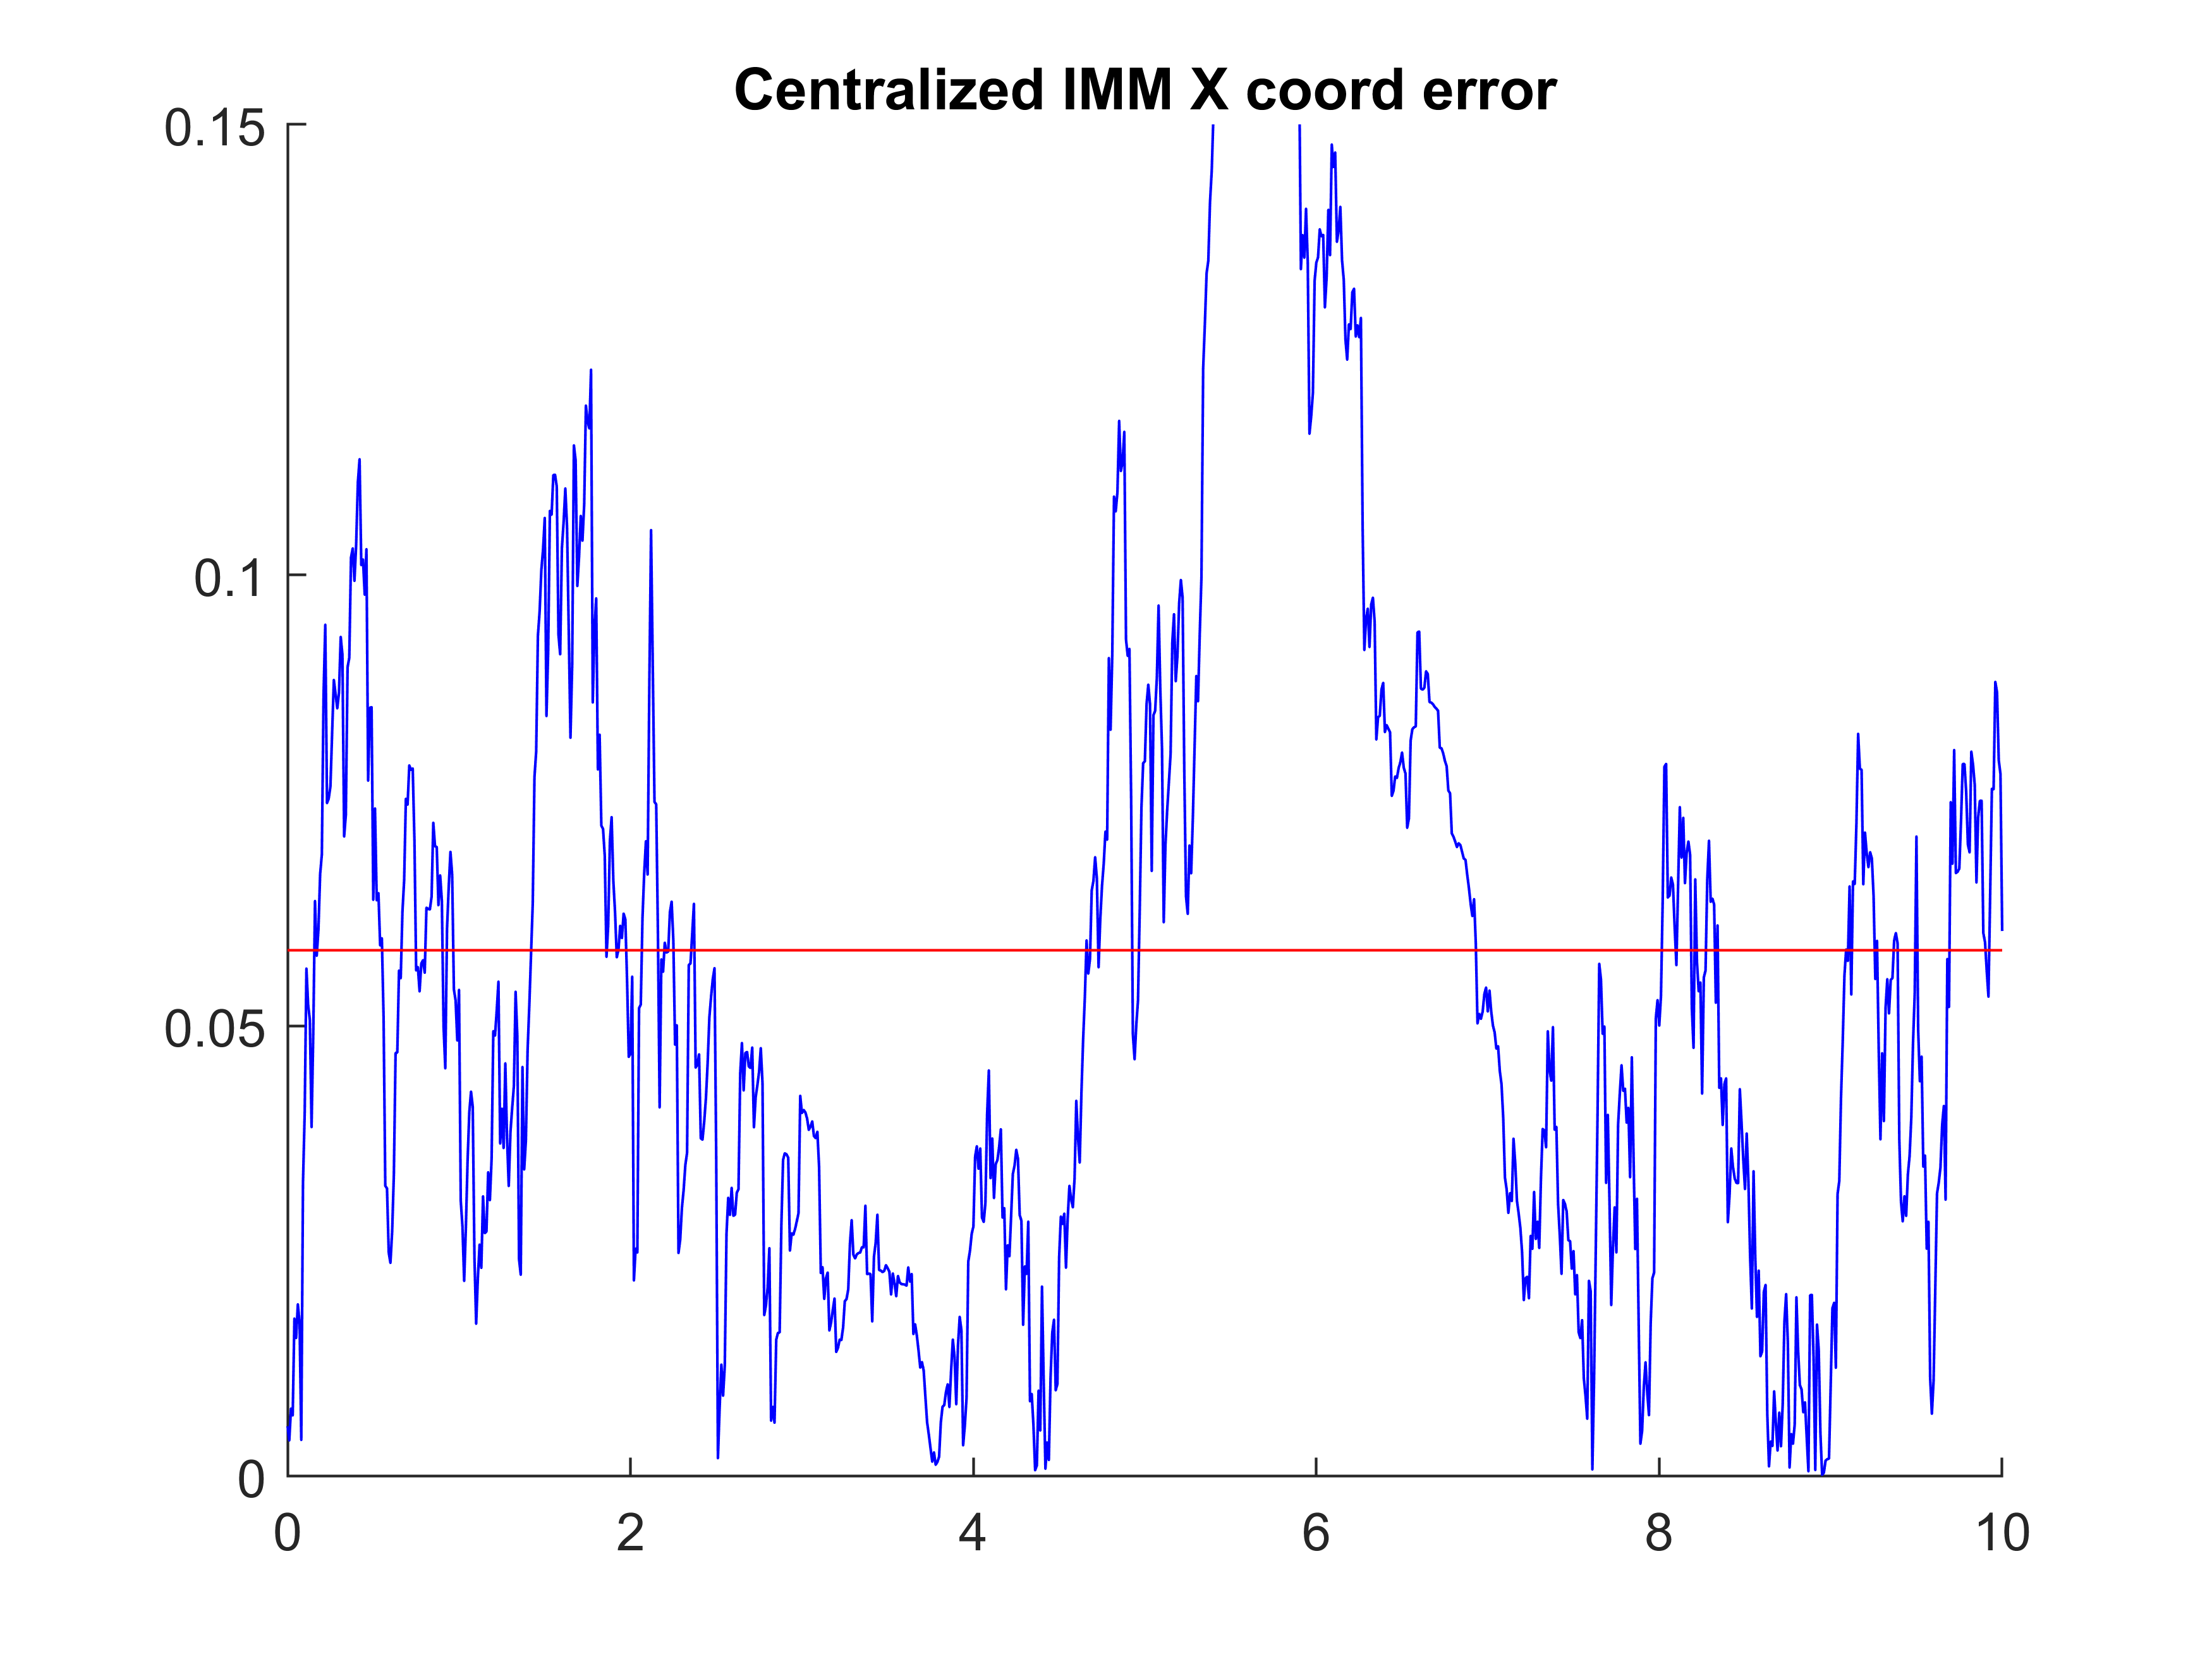
\includegraphics[width=\linewidth]{dwg/CIMM-x-error.png}
  \caption{Centralized IMM - X Error} 
\end{figure}

\begin{figure}[H]
 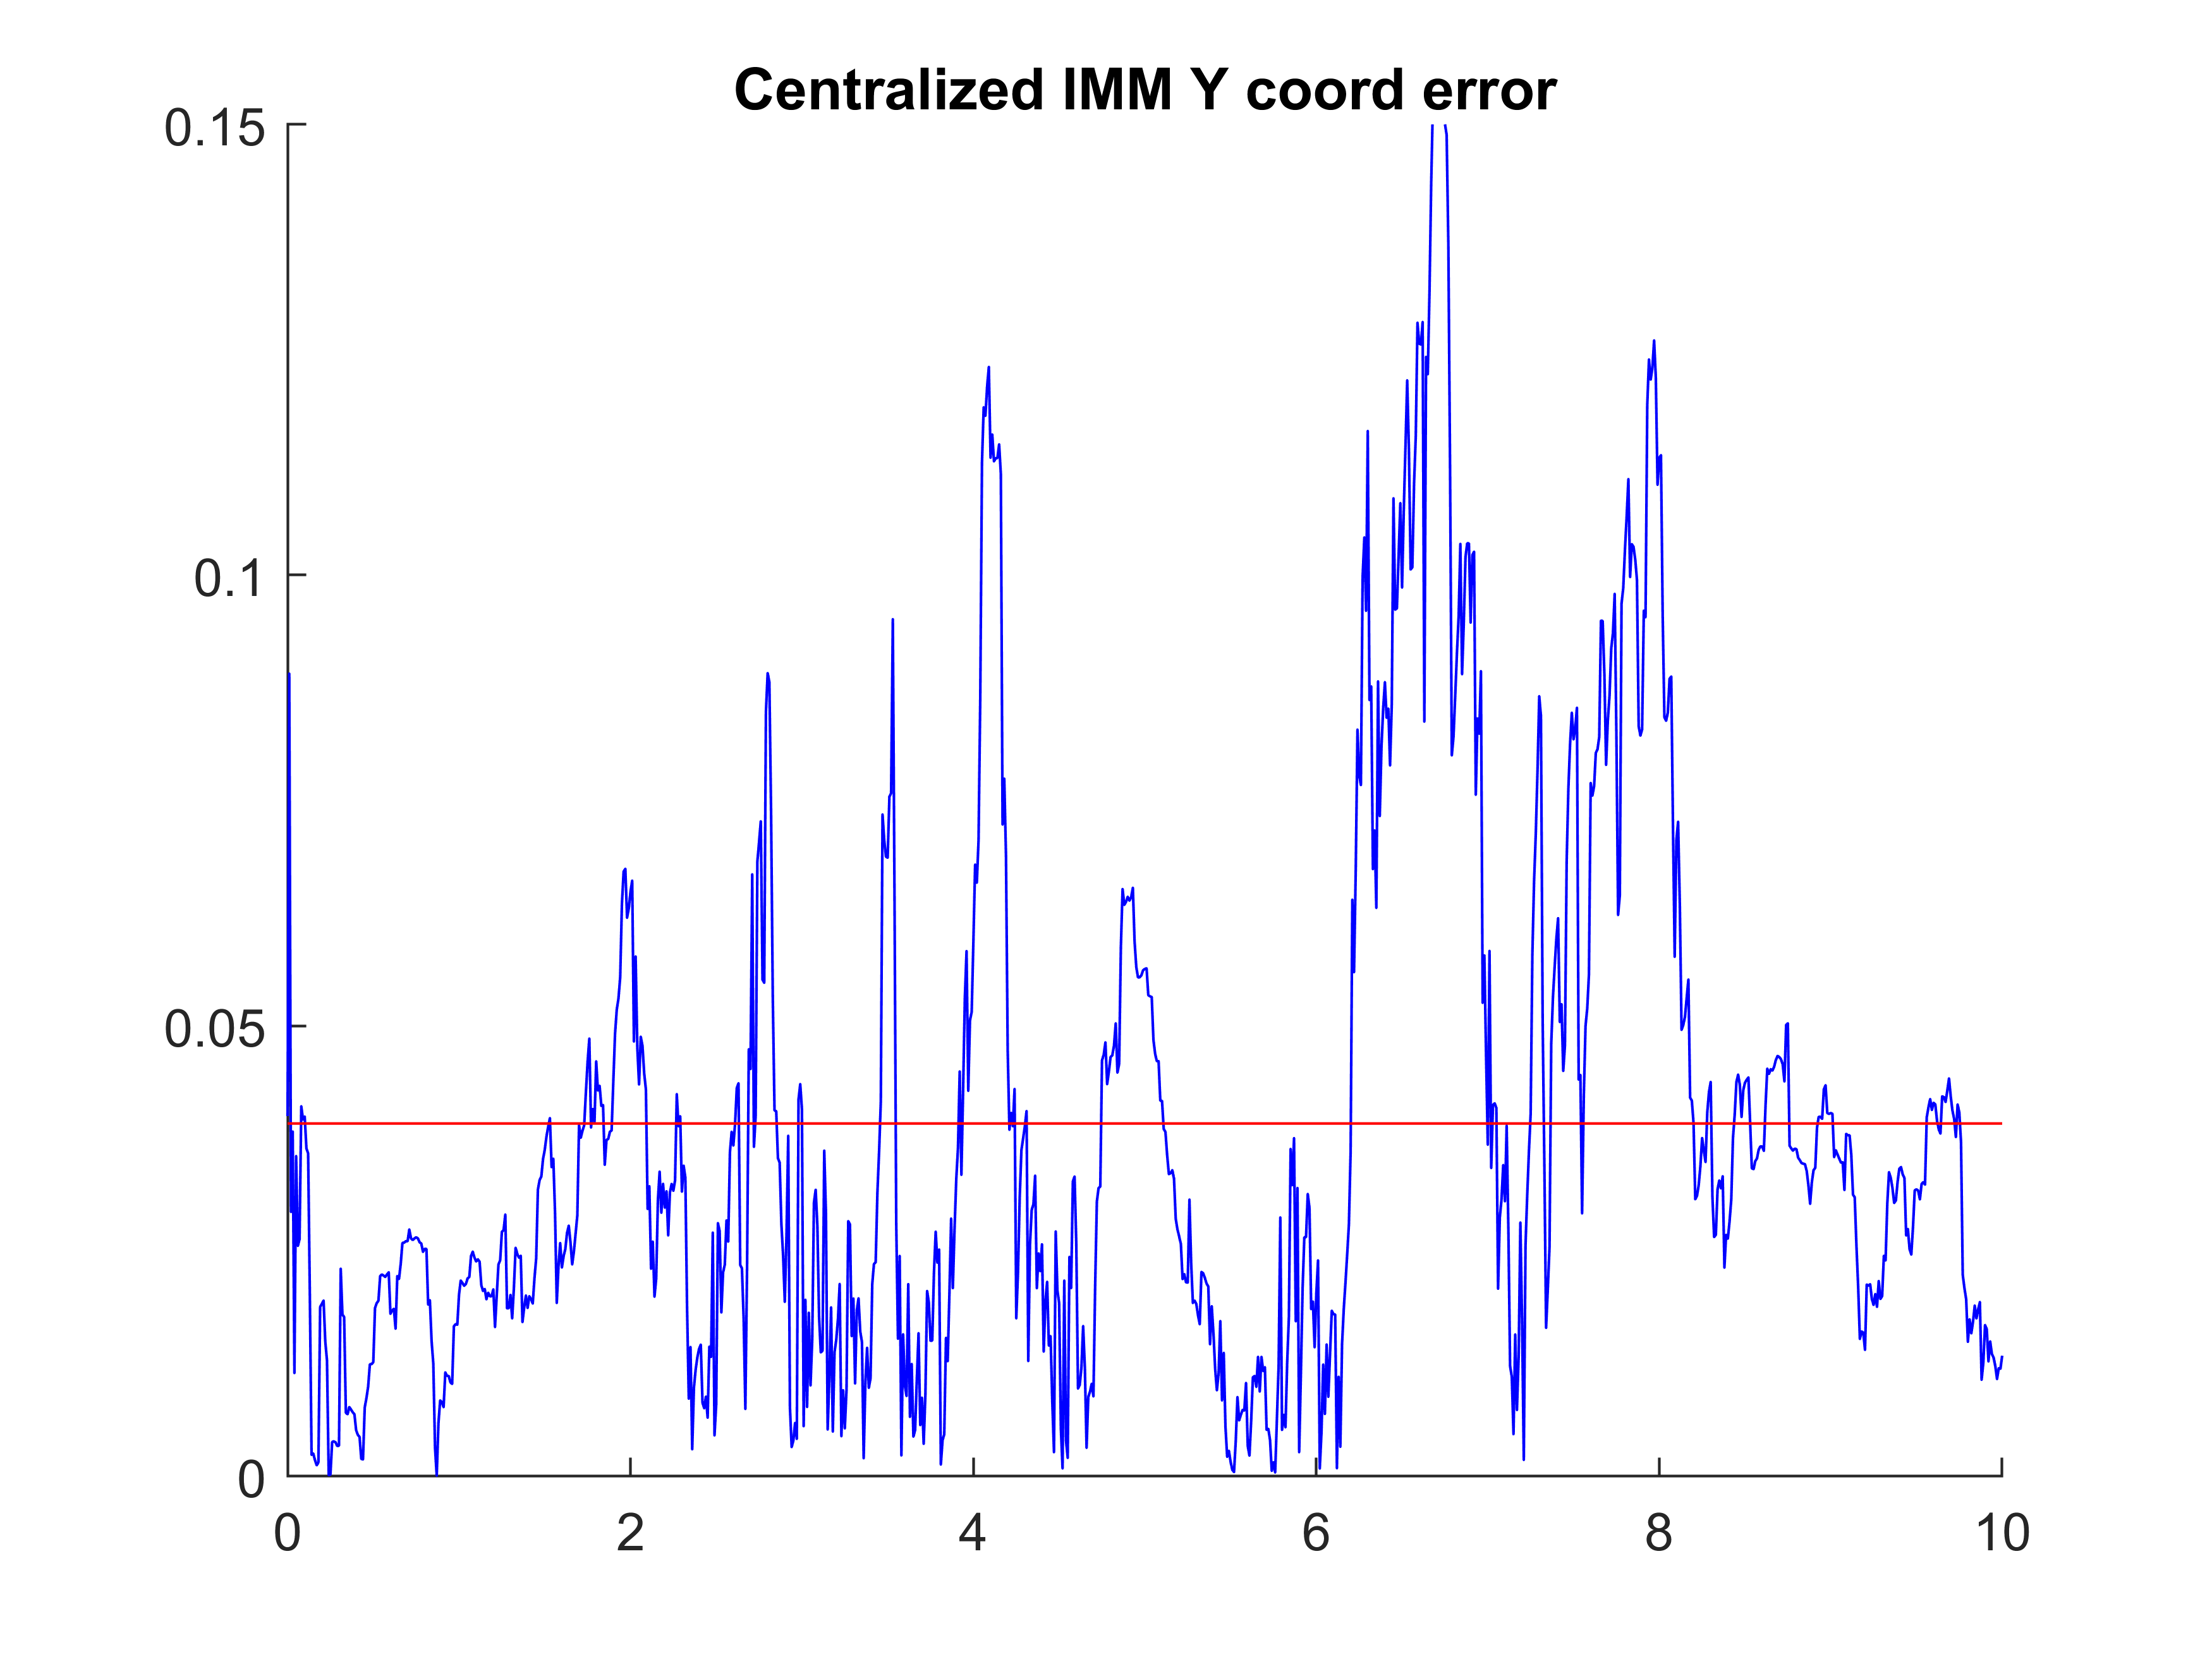
\includegraphics[width=\linewidth]{dwg/CIMM-y-error.png}
  \caption{Centralized IMM - Y Error}
 
\end{figure}

\begin{figure}[H]
 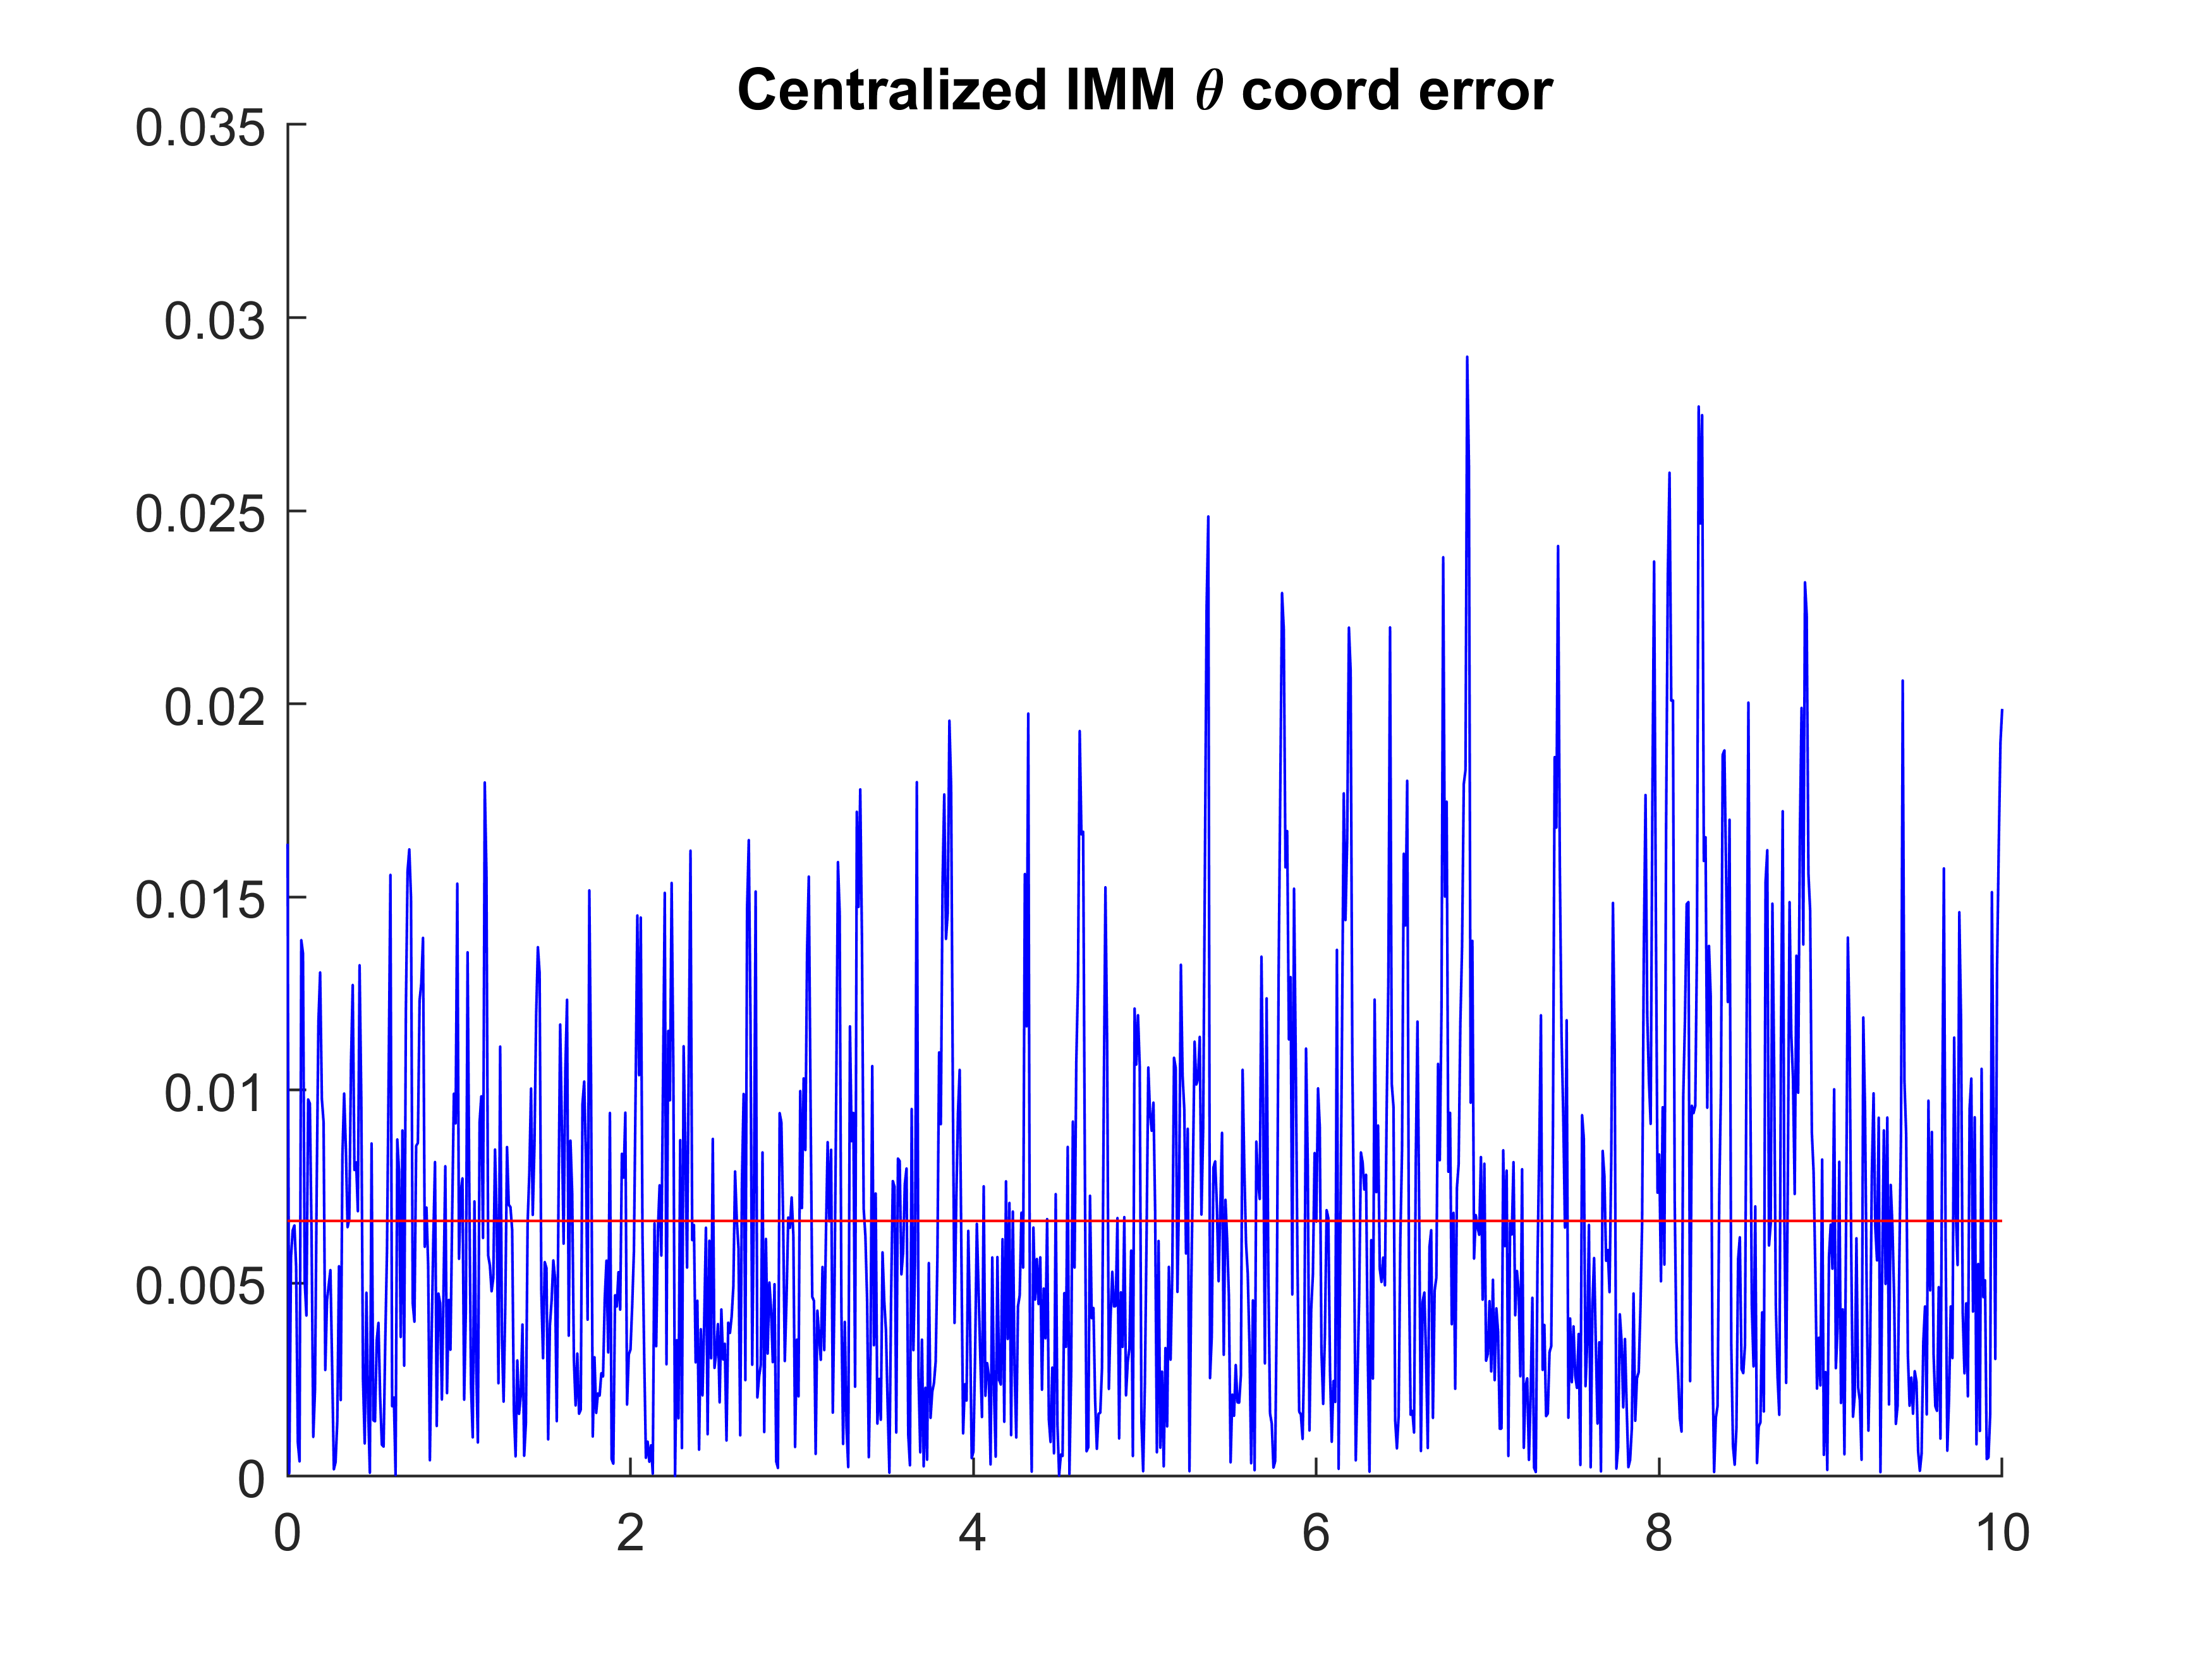
\includegraphics[width=\linewidth]{dwg/CIMM-t-error.png}
  \caption{Centralized IMM - $\Theta$ Error}
 
\end{figure}

As shown there is practically no difference in the performance of the two filter, for which we can say that the two implementation of the IMM with different expression for the Kalman Filters are equivalent to each other.
At last, we will show the probability of switching state for the IMM works in case of a fixed model for all the time and a switching model at half of the simulation.
\begin{figure}[H]
 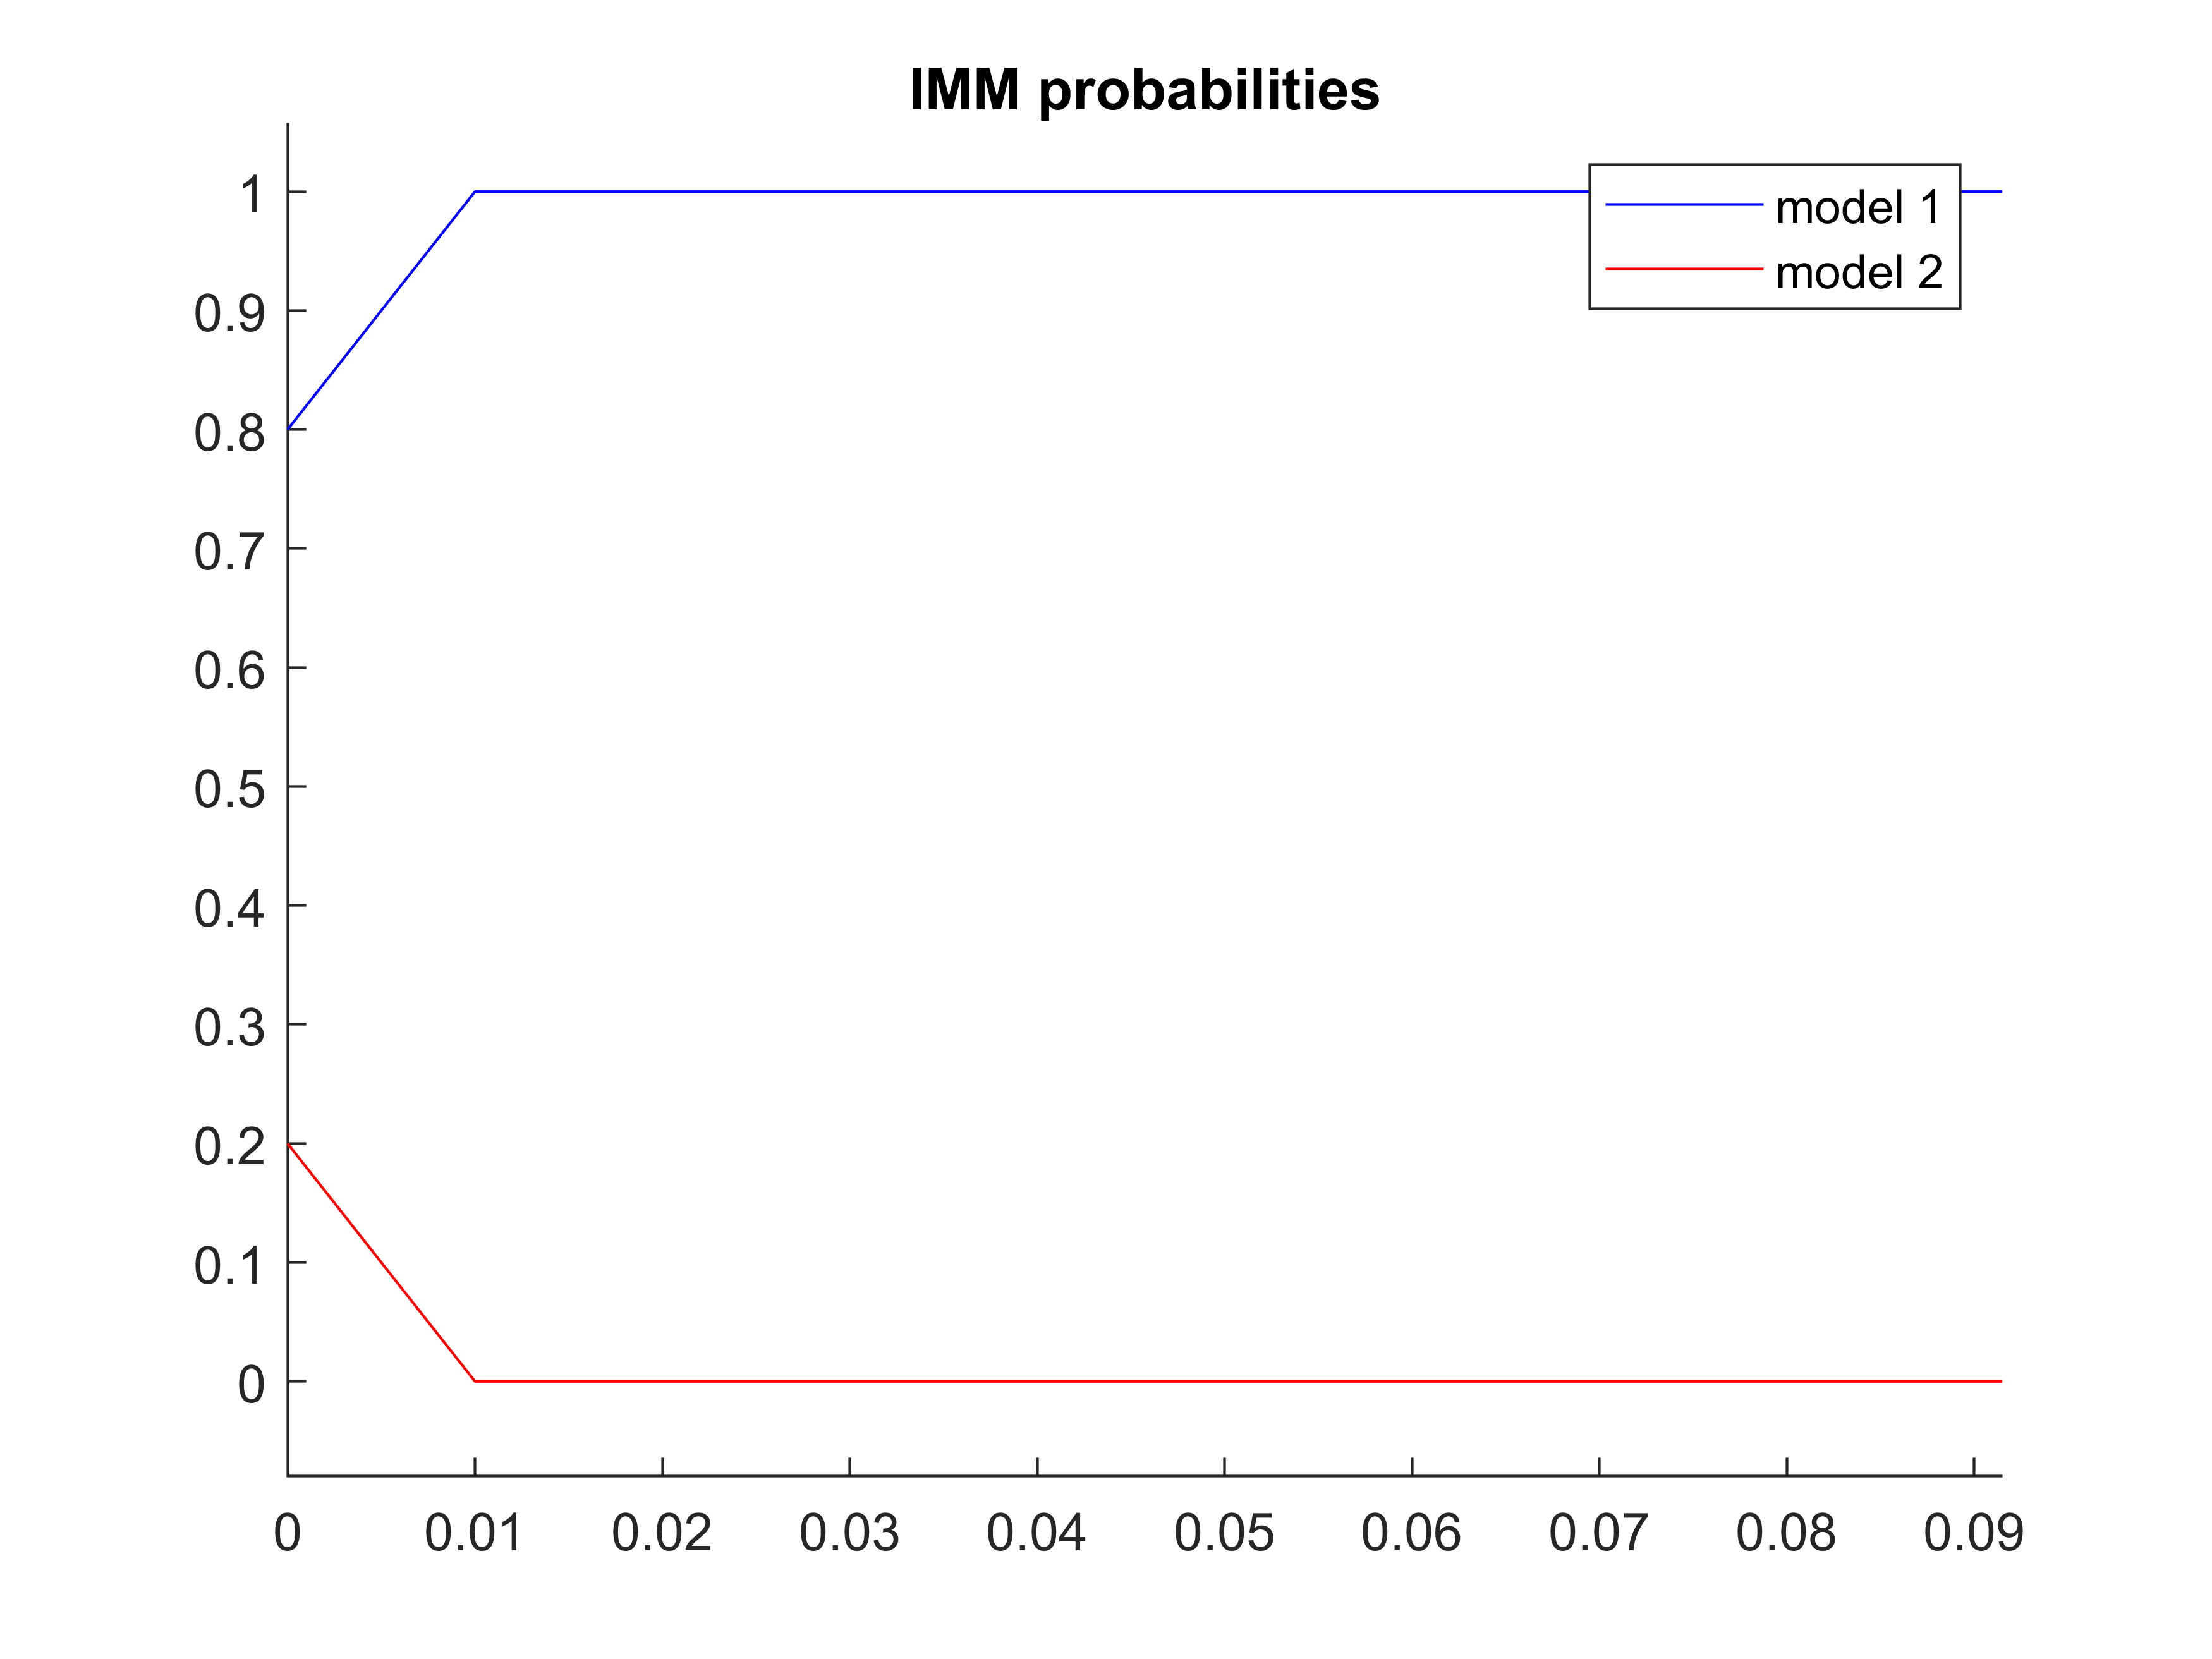
\includegraphics[width=\linewidth]{dwg/mu1.png}
  \caption{IMM - Fixed Model}
\end{figure}
\begin{figure}[H]
 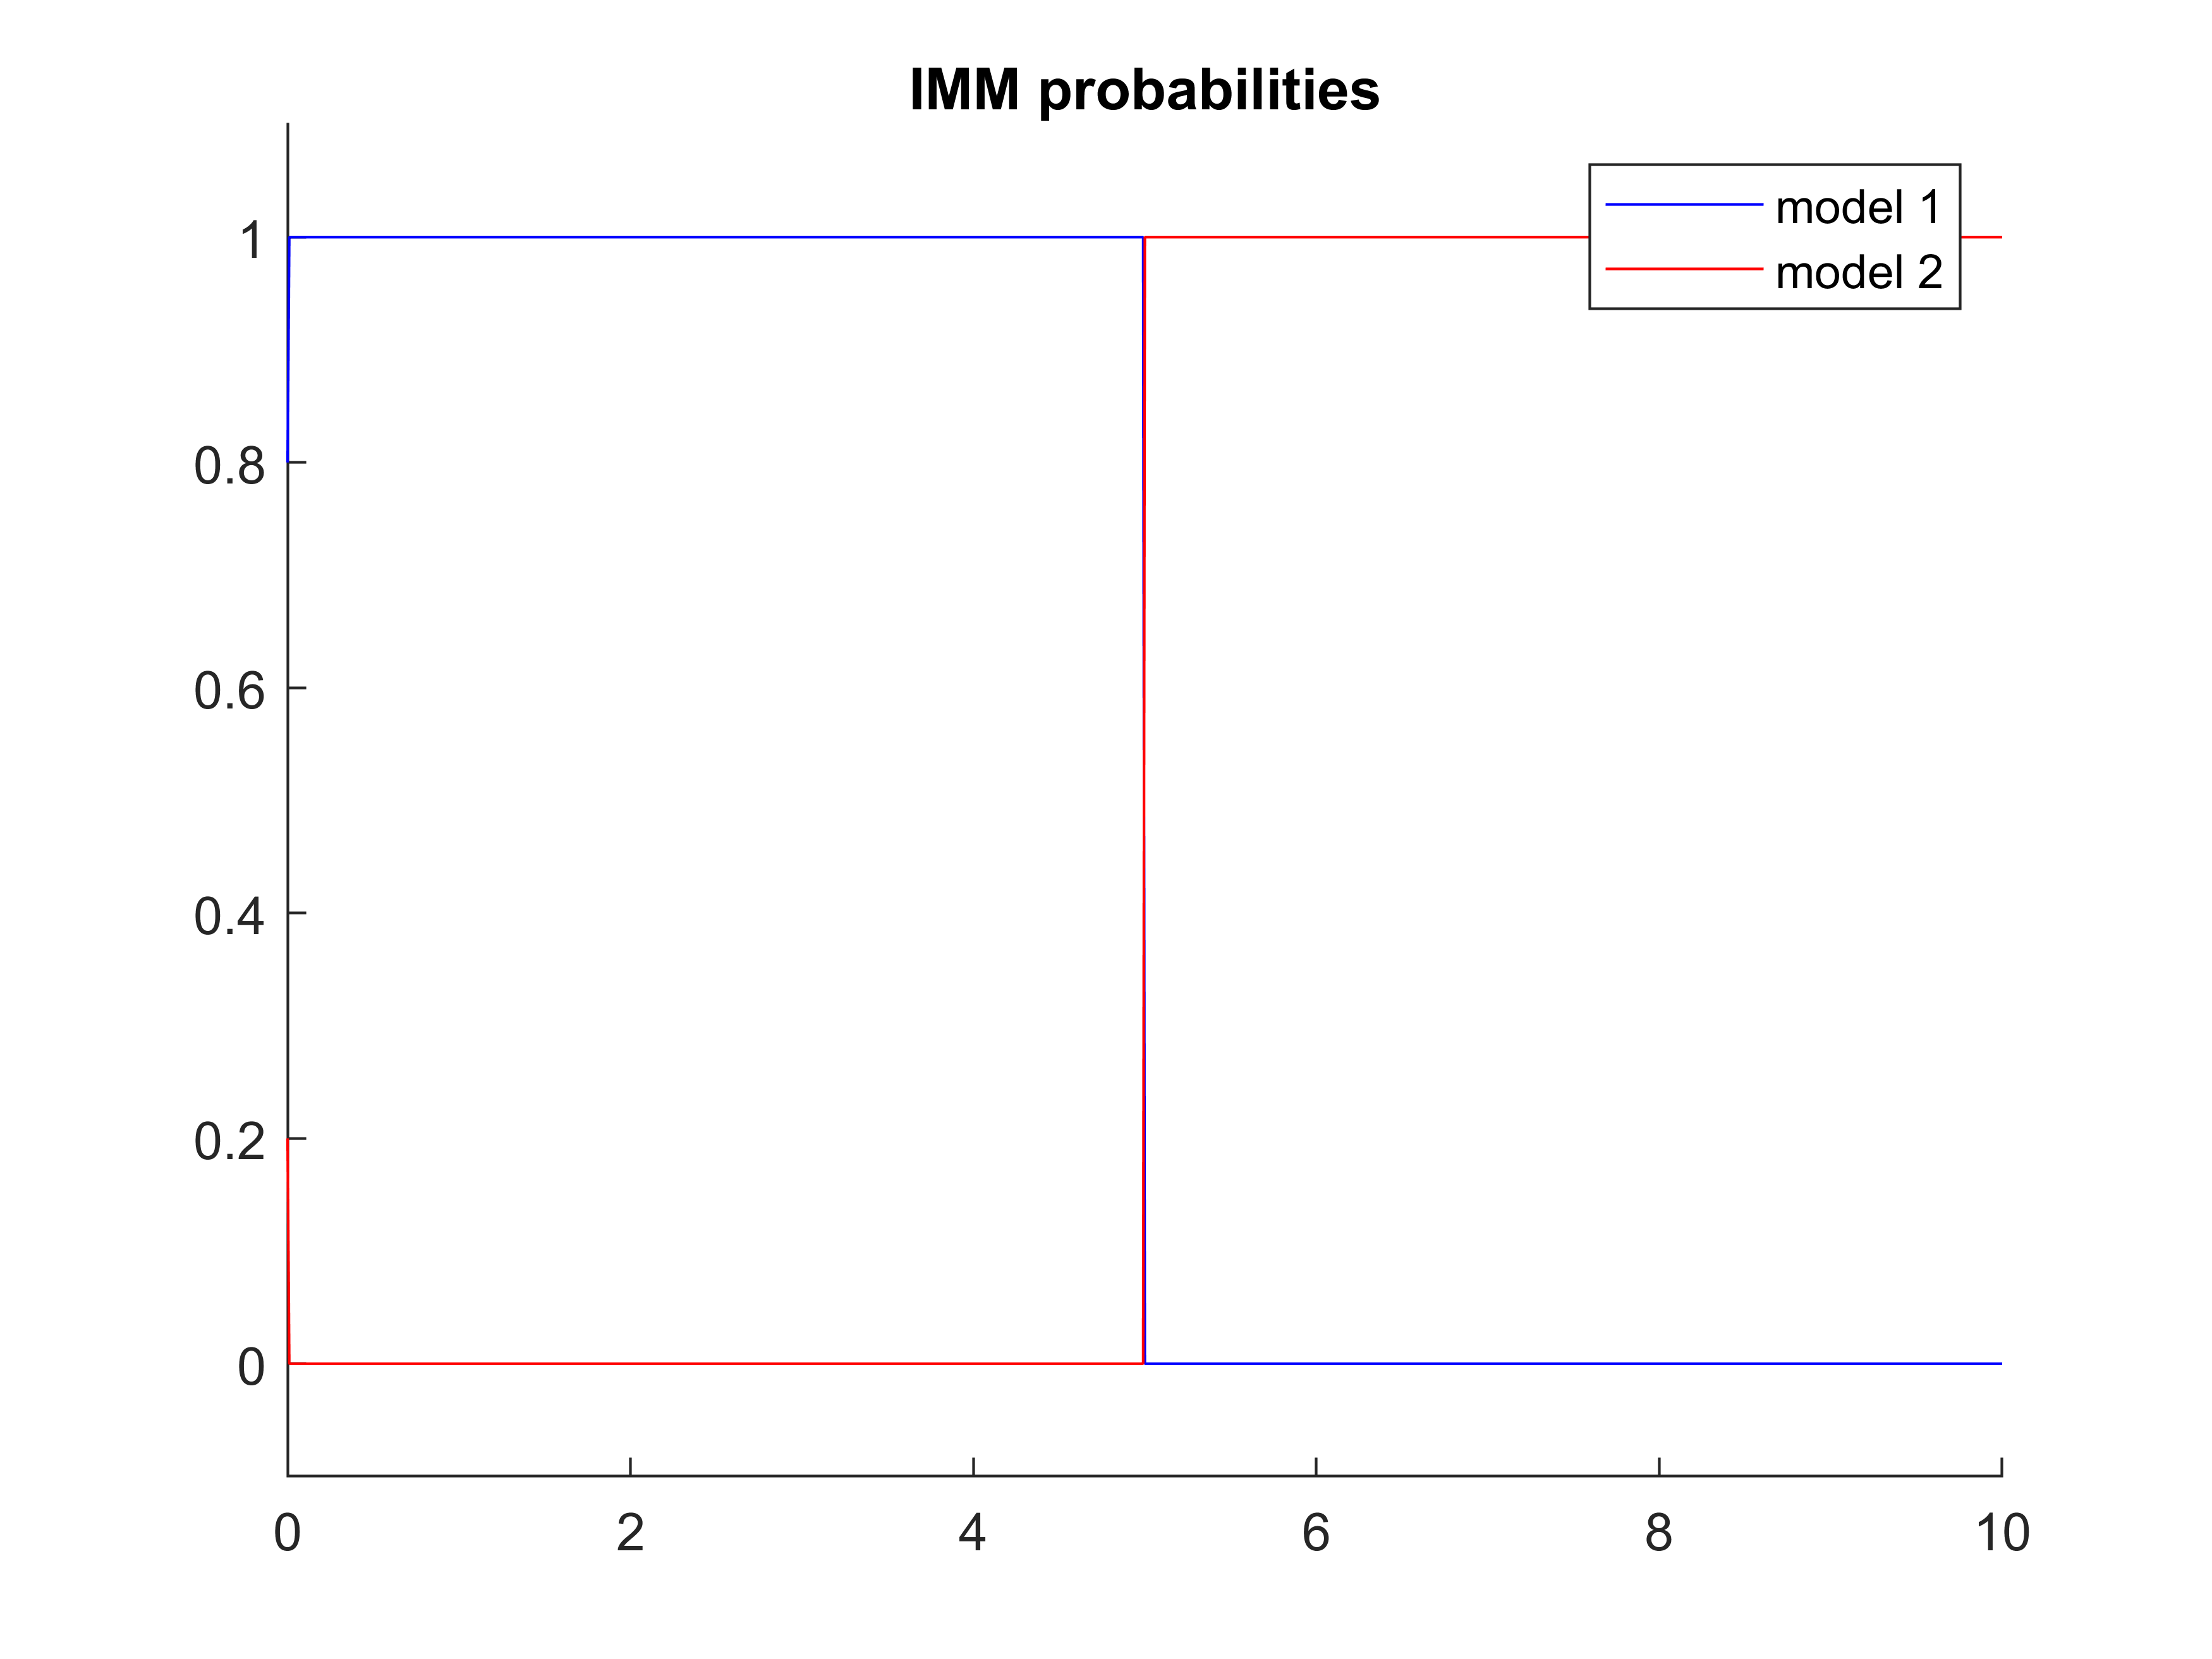
\includegraphics[width=\linewidth]{dwg/mu2.png}
  \caption{IMM - Switching Model}
\end{figure}
\begin{figure}[H]
 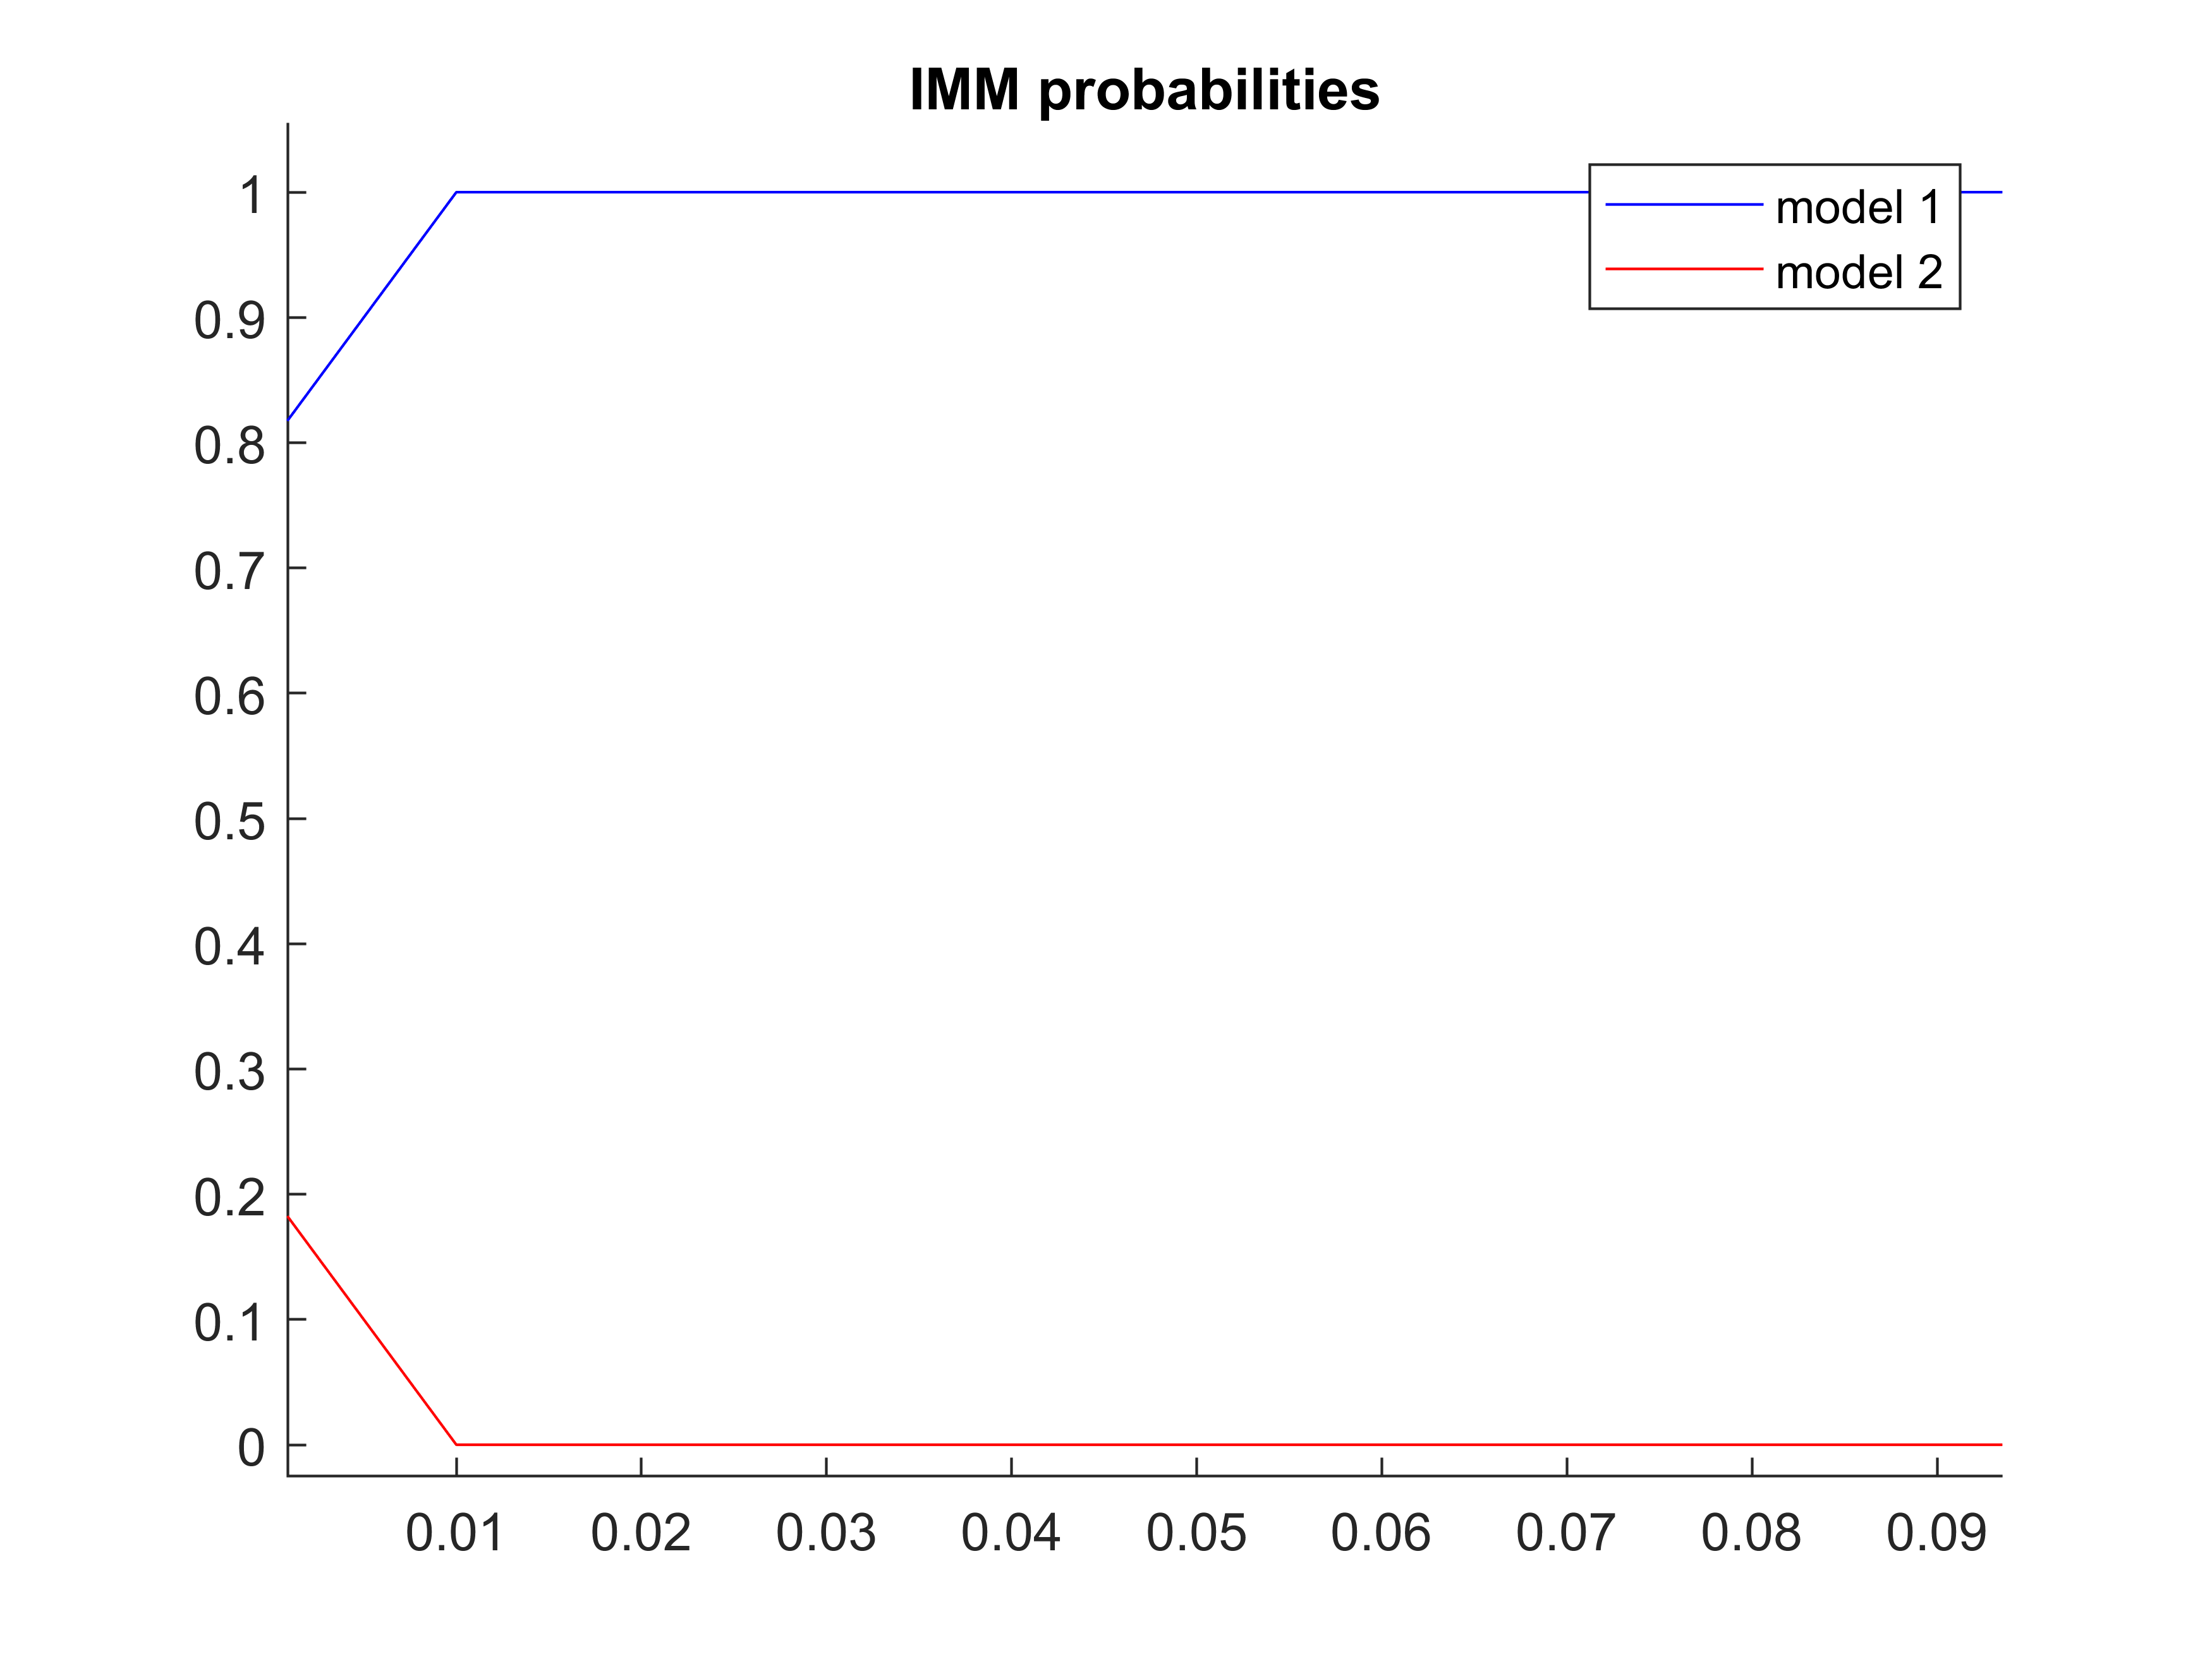
\includegraphics[width=\linewidth]{dwg/mu-centralized1.png}
  \caption{Centralized IMM - Fixed Model}
\end{figure}
\begin{figure}[H]
 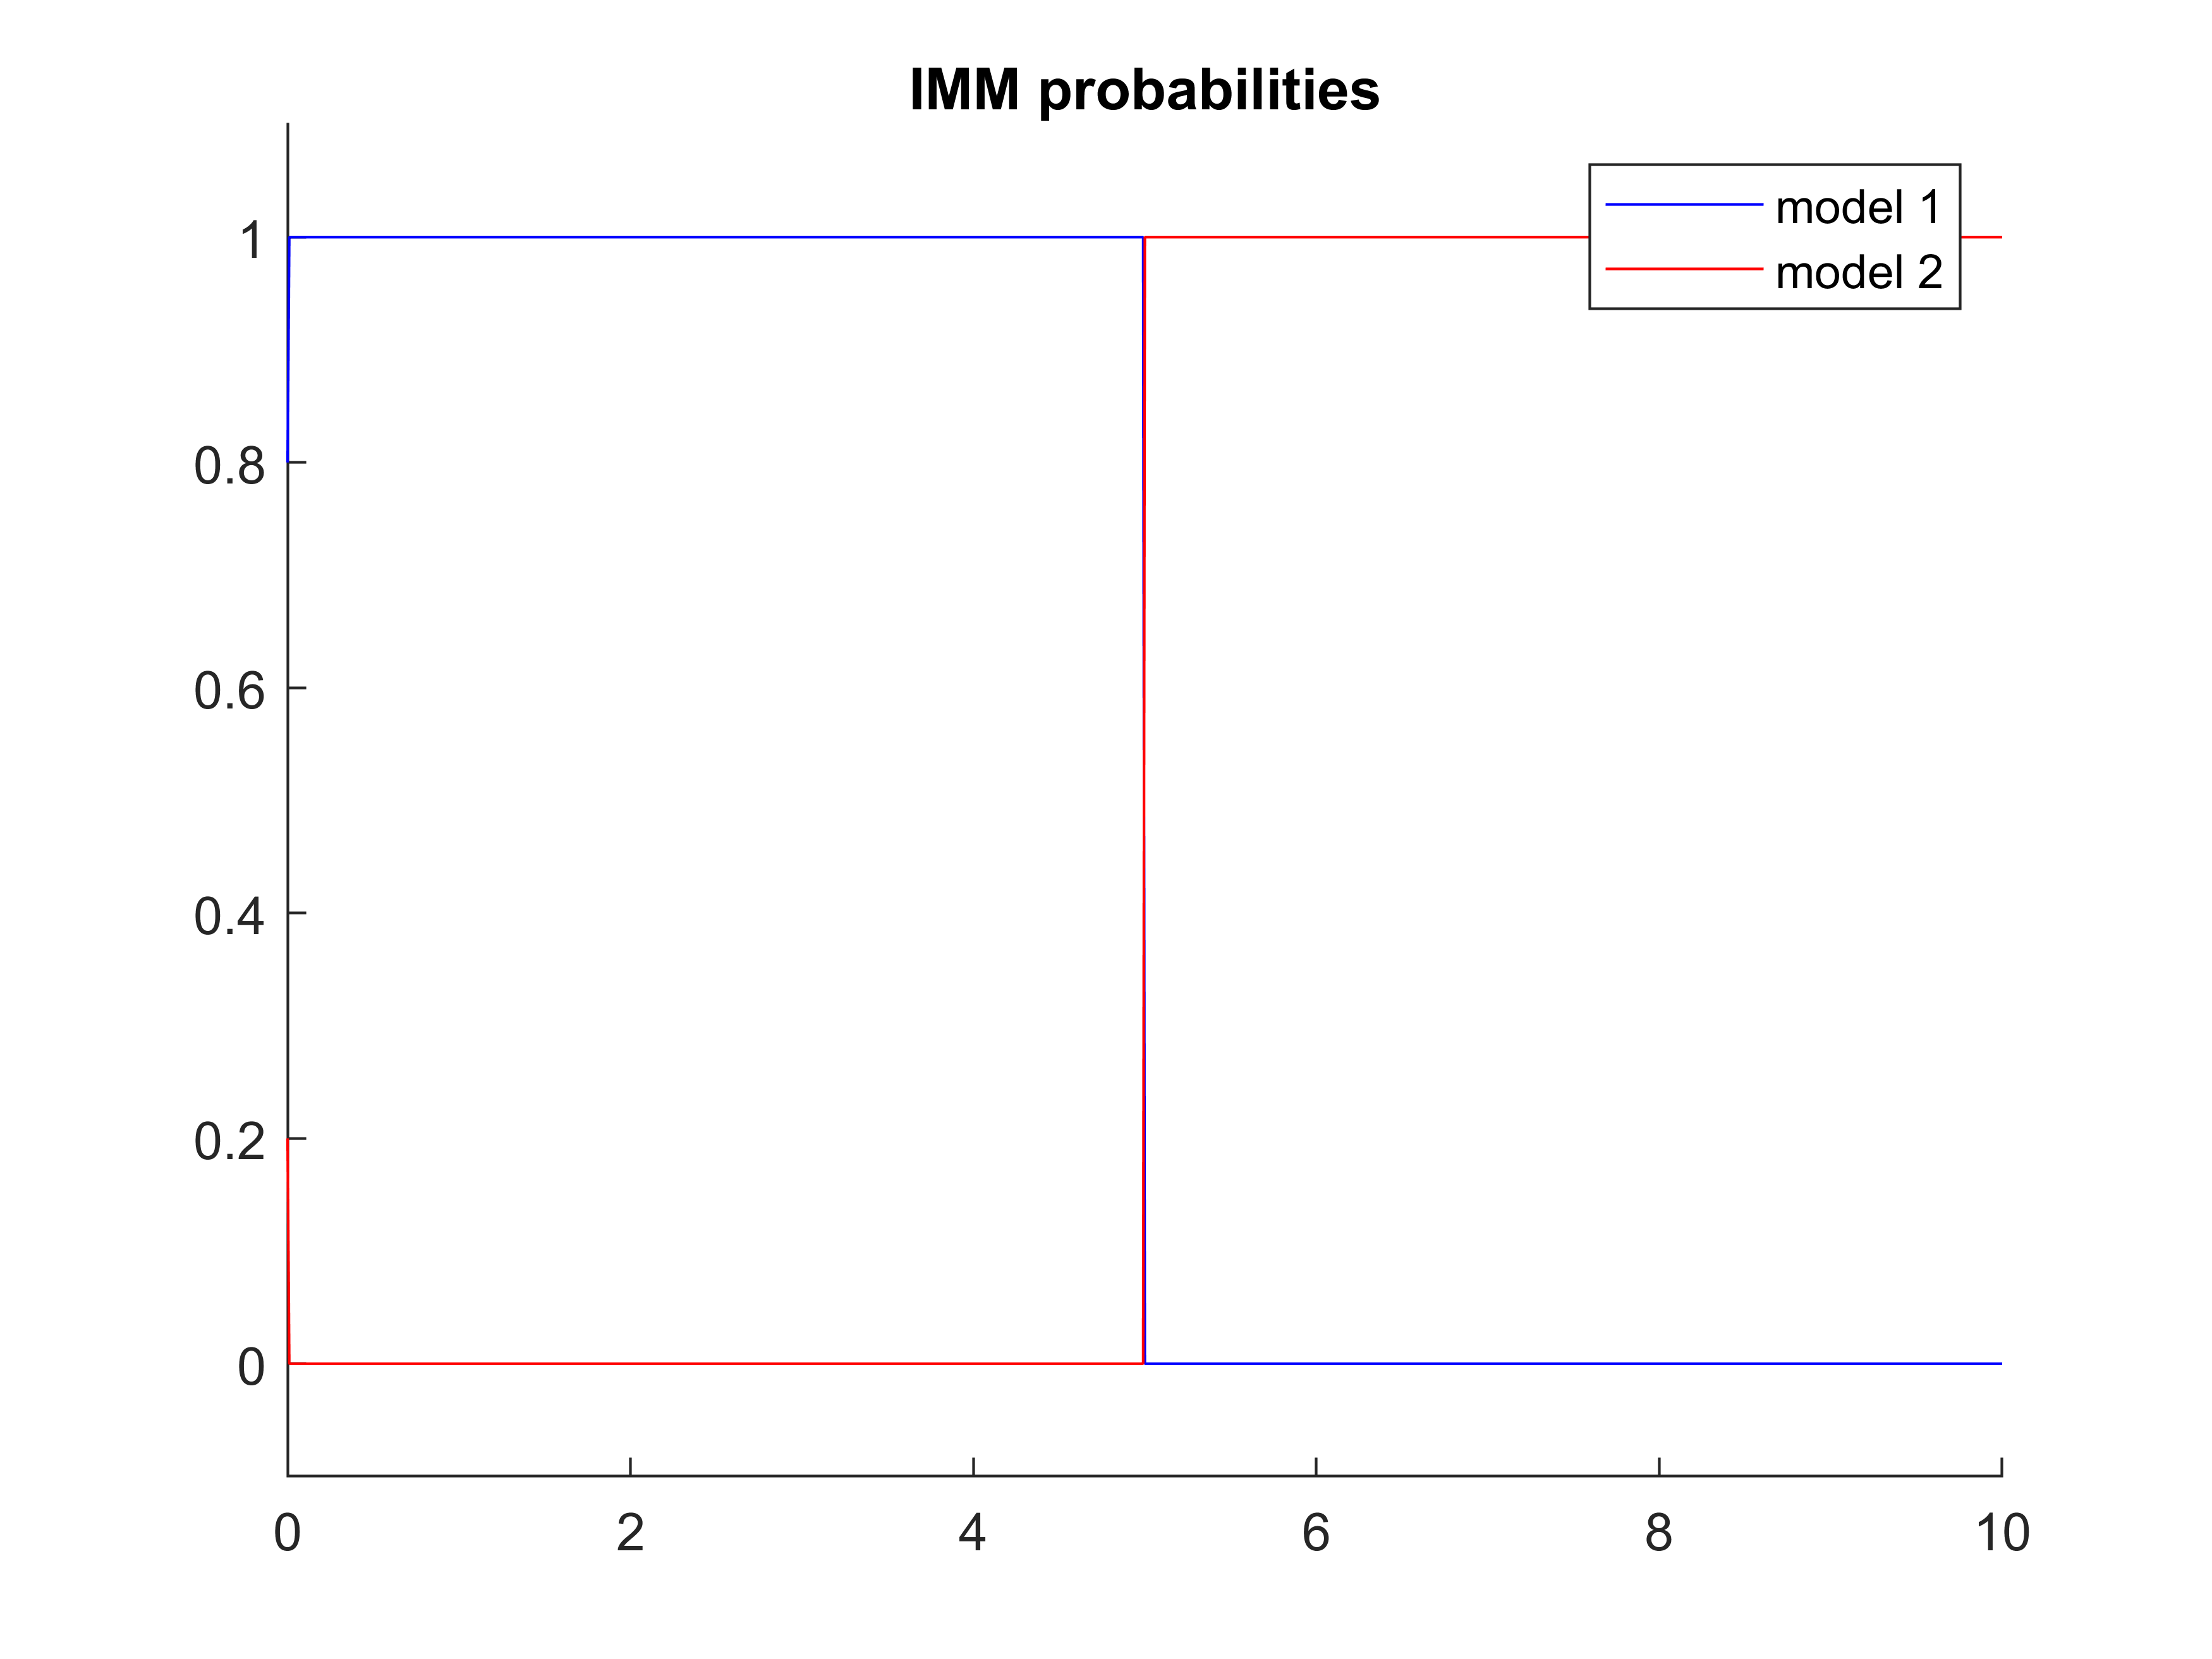
\includegraphics[width=\linewidth]{dwg/mu-centralized2.png}
  \caption{Centralized IMM - Switching Model}
 
\end{figure}


\section{Conclusion}

From this simulation, we can assess that using a Centralized form of the Kalman Filter which which divides the Kalman Filter matrices for every single agent, is basically equivalent to use a simple Kalman Filter which contains all the agents in the network as a single system.
The next step of this project will be in porting this results to the Distributed form of the Kalman Filter discussed in \cite{Kia-Martinez}. This should be an interesting case since the Algorithm proposed by Kia-Rounds-Martinez makes use of an intermediate cross covariance matrix for the update step of the Kalman Filter in the case of a relative measurement before computing the actual updated matrix. The intermediate matrix is not modified by the IMM estimator and thus some more calculation have to be done to get a working version of the Distributed algorithm. Other updates that will be proposed for the model are the possibility of loss for the measurements in some random step of the filter and keeping track of the actual distances between agents as to implment a maximum range for the measurements and the communication.

\begin{figure}[H]
 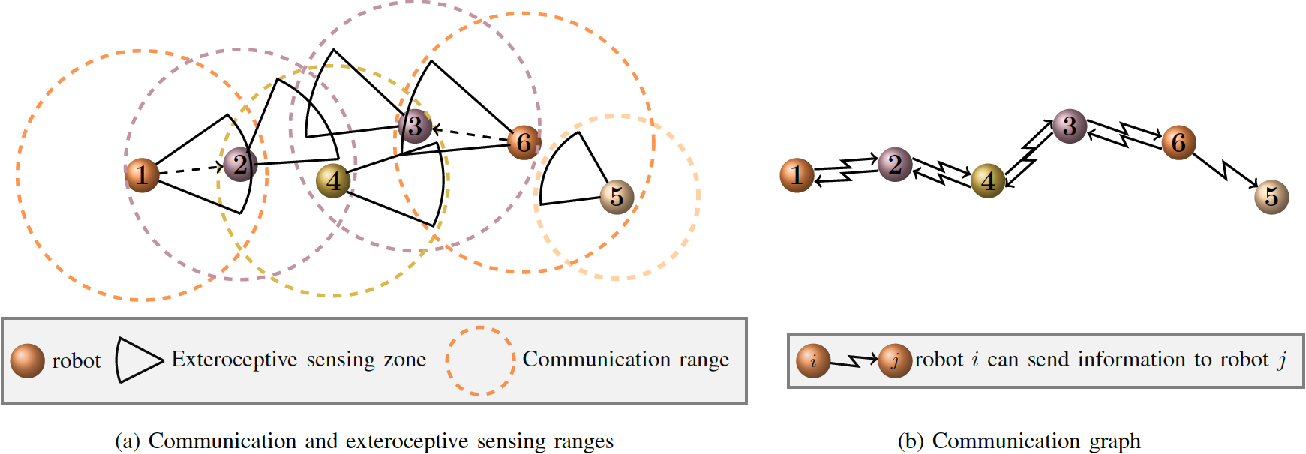
\includegraphics[width=\linewidth]{dwg/sensor-range.png}
  \caption{Sensor and communication range model}
\end{figure}

\begin{thebibliography}{9}
\bibitem{Bar-Shalom} 
Yaakov Bar-Shalom, X Rong Li, and T Kirubarajan. 
\textit{Estimation with Applications to Tracking and Navigation}. 
Wiley-Interscience; 1 edition (April 21, 2008).
 
\bibitem{Kia-Martinez} 
Solmaz S. Kia, Stephen Rounds, and Sonia Martinez.
\textit{Cooperative Localization for Mobile Agents}. 
\\\texttt{https://ieeexplore.ieee.org\\/stamp/stamp.jsp?tp=\&arnumber=7434174\&tag=1}


\end{thebibliography}






%
%\section{Algorithm}
%
%Initialize the filter both filter at k=0: \\
%$\forall$ i = 1..r : r = number of agents and j $\ne$ i
%
%$$ \hat{x}_{a}^{i+}(0) \in R^{n} , \hat{P}_{a}^{i+}(0) \in R^{n x n} , \hat{P}_{a}^{ij+}(0) = 0_{n x n}$$
%$$ \hat{x}_{b}^{i+}(0) \in R^{n} , \hat{P}_{b}^{i+}(0) \in R^{n x n} , \hat{P}_{b}^{ij+}(0) = 0_{n x n}$$
%
%Initialize IMM parameters as:
%
%$$ \Pi = \begin{bmatrix} 0.85 & 0.15 \\ 0.15 &0.85 \end{bmatrix}$$
%$$ \hat{\mu}(0) = \begin{bmatrix} 0.7 \\ 0.3  \end{bmatrix}$$
%
%
%Then for each k$>$ 0 do: \\
%\\
%
%Update  $\tilde{\mu}$(k):
%
%$$ \psi(k) = \Pi \cdot \hat{\mu}(k) $$
%
%$$ \tilde{\mu}^{1,a}(k) =  \frac{1}{\psi^{a}} \cdot \Pi(1,a) \cdot \hat{\mu}^{1}(k) $$
%$$ \tilde{\mu}^{2,a}(k) =  \frac{1}{\psi^{a}} \cdot \Pi(2,a) \cdot \hat{\mu}^{2}(k) $$
%$$ \tilde{\mu}^{1,b}(k) =  \frac{1}{\psi^{b}} \cdot \Pi(1,b) \cdot \hat{\mu}^{1}(k) $$
%$$ \tilde{\mu}^{2,b}(k) =  \frac{1}{\psi^{b}} \cdot \Pi(2,b) \cdot \hat{\mu}^{2}(k) $$
% State Interaction for IMM:
%
%$$ \hat{x}^{0}_{a}(k)  = \hat{x}_{a}^{+}(k)\cdot \tilde{\mu}^{1,a}(k) + \hat{x}_{b}^{+}(k) \cdot \tilde{\mu}^{2,a}(k) $$ 
%
%$$ \hat{x}^{0}_{b}(k)  = \hat{x}_{a}^{+}(k) \cdot \tilde{\mu}^{1,b} + \hat{x}_{b}^{+}(k) \cdot \tilde{\mu}^{2,b}(k) $$ 
%
%
%$$ \hat{P}^{0}_{a}(k) = [ \hat{P}_{a}^{+}(k)+(\hat{x}_{a}^{+}(k)-\hat{x}^{0}_{a}(k)) \cdot (\hat{x}_{a}^{+}(k)-\hat{x}^{0}_{a}(k))^{T}]\cdot \tilde{\mu}^{1,a}(k) $$ 
%$$+ [ \hat{P}_{b}^{+}(k)+(\hat{x}_{b}^{+}(k)-\hat{x}^{0}_{a}(k)) \cdot (\hat{x}_{b}^{+}(k)-\hat{x}^{0}_{a}(k))^{T}]\cdot \tilde{\mu}^{2,a}(k)  $$
%
%
%$$ \hat{P}^{0}_{b}(k) = [ \hat{P}_{a}^{+}(k)+(\hat{x}_{a}^{+}(k)-\hat{x}^{0}_{b}(k)) \cdot (\hat{x}_{a}^{+}(k)-\hat{x}^{0}_{b}(k))^{T}]\cdot \tilde{\mu}^{1,b}(k) $$ 
%$$+ [ \hat{P}_{b}^{+}(k)+(\hat{x}_{b}^{+}(k)-\hat{x}^{0}_{b}(k)) \cdot (\hat{x}_{b}^{+}(k)-\hat{x}^{0}_{b}(k))^{T}]\cdot \tilde{\mu}^{2,b}(k)  $$
%
%Prediction Step for both Kalman Filters:
%
%$\forall$ i = 1..r : r = number of agents and j $\ne$ i
%
%$$ \hat{x}_{a}^{i-}(k+1) = f^{i}(x^{i0}_{a}(k),u^{i}(k)) $$
%$$  \hat{P}_{a}^{i-}(k+1) = A^{i}(k) \cdot \hat{P}_{a}^{i0}(k) \cdot A^{i}(k)^{T} + B^{i}(k) \cdot Q^{i}(k) \cdot B^{i}(k)^{T}$$
%$$  \hat{P}_{a}^{ij-}(k+1) = A^{i}(k) \cdot \hat{P}_{a}^{ij0}(k) \cdot A^{j}(k)^{T} $$
%
%$$ \hat{x}_{b}^{i-}(k+1) = f^{i}(x^{i0}_{b}(k),u^{i}(k)) $$
%$$  \hat{P}_{b}^{i-}(k+1) = A^{i}(k) \cdot \hat{P}_{b}^{i0}(k) \cdot A^{i}(k)^{T} + B^{i}(k) \cdot Q^{i}(k) \cdot B^{i}(k)^{T}$$
%$$  \hat{P}_{b}^{ij-}(k+1) = A^{i}(k) \cdot \hat{P}_{b}^{ij0}(k) \cdot A^{j}(k)^{T} $$
%
%Relative or absolute measurement is taken in both filters:
%measurement between agent  i and j $\ne$ i
%
%$$r_{a}^{ij}(k+1) = h(x^{i}_{a}(k+1),x^{j}_{a}(k+1)) -  h(\hat{x}_{a}^{i-}(k+1),\hat{x}_{a}^{j-}(k+1))$$
%$$r_{b}^{ij}(k+1) = h(x^{i}_{b}(k+1),x^{j}_{b}(k+1)) -  h(\hat{x}_{b}^{i-}(k+1),\hat{x}_{b}^{j-}(k+1))$$
%
%Find Residual Covariance for both filters:
%
%$$S_{a}^{ij}(k+1) = R_{a}(k+1) + H_{a}^{i}(k+1) \cdot  \hat{P}_{a}^{i-}(k+1)  \cdot  H_{a}^{i}(k+1)^{T}+$$
%$$H_{a}^{j}(k+1) \cdot  \hat{P}_{a}^{j-}(k+1)  \cdot  H_{a}^{j}(k+1)^{T} -$$
%$$H_{a}^{i}(k+1) \cdot  \hat{P}_{a}^{ij-}(k+1)  \cdot  H_{a}^{j}(k+1)^{T}-$$
%$$H_{a}^{j}(k+1) \cdot  \hat{P}_{a}^{ij-}(k+1)^{T}  \cdot  H_{a}^{i}(k+1)^{T}$$
%$$S_{b}^{ij}(k+1) = R_{a}(k+1) + H_{a}^{i}(k+1) \cdot  \hat{P}_{a}^{i-}(k+1)  \cdot  H_{a}^{i}(k+1)^{T}+$$
%$$H_{b}^{j}(k+1) \cdot  \hat{P}_{b}^{j-}(k+1)  \cdot  H_{b}^{j}(k+1)^{T} -$$
%$$H_{b}^{i}(k+1) \cdot  \hat{P}_{b}^{ij-}(k+1)  \cdot  H_{b}^{j}(k+1)^{T}-$$
%$$H_{b}^{j}(k+1) \cdot  \hat{P}_{b}^{ij-}(k+1)^{T}  \cdot  H_{b}^{i}(k+1)^{T}$$
%
%Then Kalman Gain for each agent in both filters: 
%
%$$K_{a}^{i}(k+1) = (\hat{P}_{a}^{ij-}(k+1) \cdot H_{a}^{j}(k+1)^{T}-\hat{P}_{a}^{i-}(k+1) \cdot  H_{a}^{i}(k+1)^{T}) \cdot S_{a}^{ij}(k+1)^{-1} $$
%$$K_{a}^{j}(k+1) = (\hat{P}_{a}^{j-}(k+1) \cdot H_{a}^{j}(k+1)^{T}-\hat{P}_{a}^{ij-}(k+1)^{T} \cdot  H_{a}^{i}(k+1)^{T}) \cdot S_{a}^{ij}(k+1)^{-1} $$
%
%$$K_{b}^{i}(k+1) = (\hat{P}_{b}^{ij-}(k+1) \cdot H_{b}^{j}(k+1)^{T}-\hat{P}_{b}^{i-}(k+1) \cdot  H_{b}^{i}(k+1)^{T}) \cdot S_{b}^{ij}(k+1)^{-1} $$
%$$K_{b}^{j}(k+1) = (\hat{P}_{b}^{j-}(k+1) \cdot H_{b}^{j}(k+1)^{T}-\hat{P}_{b}^{ij-}(k+1)^{T} \cdot  H_{b}^{i}(k+1)^{T}) \cdot S_{b}^{ij}(k+1)^{-1} $$
%
%Model Probability Update:
%
%$$ \Lambda_{a}(k+1) = \frac{1}{\sqrt{|2  \pi  S_{a}^{ij}(k+1)|}}\cdot e^{- \frac{1}{2} r_{a}^{ij}(k+1)^{T}  S_{a}^{ij}(k+1) r_{a}^{ij}(k+1) }$$
%
%$$ \Lambda_{b}(k+1) = \frac{1}{\sqrt{|2  \pi  S_{b}^{ij}(k+1)|}}\cdot e^{- \frac{1}{2} r_{b}^{T}  S_{b}^{ij}(k+1) r_{b} }$$
%
%$$ c = \Lambda_{a}(k+1) \bar{c}_{a} + \Lambda_{b}(k+1) \bar{c}_{b} $$
%
%$$\hat{\mu}^{1}(k+1) = \frac{1}{c} \Lambda_{a}(k+1) \bar{c}_{a} $$
%$$\hat{\mu}^{2}(k+1) = \frac{1}{c} \Lambda_{b}(k+1) \bar{c}_{b} $$
%
%Update Step for each Kalman Filter: \\
%$\forall$ i = 1..r : r = number of agents and j $\ne$ i
%
%$$ \hat{x}_{a}^{i+}(k+1) = {x}_{a}^{i-}(k+1)+K_{a}^{i}(k+1) r_{a}(k+1)$$
%$$  \hat{P}_{a}^{i+}(k+1) = \hat{P}_{a}^{i-}(k+1)-K_{a}^{i}(k+1) S_{a}^{ij}(k+1) K_{a}^{i}(k+1)^{T}$$
%$$  \hat{P}_{a}^{ij+}(k+1) = \hat{P}_{a}^{ij-}(k+1)-K_{a}^{i}(k+1) S_{a}^{ij}(k+1) K_{a}^{j}(k+1)^{T}$$
%
%$$ \hat{x}_{b}^{i+}(k+1) = {x}_{b}^{i-}(k+1)+K_{b}^{i}(k+1) r_{b}(k+1)$$
%$$  \hat{P}_{b}^{i+}(k+1) = \hat{P}_{b}^{i-}(k+1)-K_{b}^{i}(k+1) S_{b}^{ij}(k+1) K_{b}^{i}(k+1)^{T}$$
%$$  \hat{P}_{b}^{ij+}(k+1) = \hat{P}_{b}^{ij-}(k+1)-K_{b}^{i}(k+1) S_{b}^{ij}(k+1) K_{b}^{j}(k+1)^{T}$$
%
%
%Combine State Estimation for IMM:
%
%$$ \hat{x}^{IMM}(k+1) = {x}_{a}^{+}(k+1) \hat{\mu}^{1}(k+1) +  \hat{x}_{b}^{+}(k+1) \hat{\mu}^{2}(k+1) $$
%
%$$  \hat{P}^{IMM}(k+1) =\hat{\mu}^{1}(k+1) [ \hat{P}_{a}(k+1)+( \hat{x}_{a}(k+1)  -  \hat{x}^{IMM}(k+1))( \hat{x}_{a}(k+1)  -  \hat{x}^{IMM}(k+1))^{T}]+ $$
%$$\hat{\mu}^{2}(k+1) [ \hat{P}_{b}(k+1)+( \hat{x}_{b}(k+1)  -  \hat{x}^{IMM}(k+1))( \hat{x}_{b}(k+1)  -  \hat{x}^{IMM}(k+1))^{T}] $$
%
%-$>$ k = k+1
\end{document}
